\documentclass[11pt,letterpaper]{article}%another class might be appropriate, but I'm most familiar with article

%PACKAGES 
%\usepackage[english]{babel}     <--why don't we use these?
%\usepackage[utf8x]{inputenc}
\usepackage{siunitx}%si unit typesetting
\usepackage{amsmath}%math typesetting stuff
\usepackage{fancyhdr}%header & footer stuff
\usepackage{cancel}%for canceling out stuff in formulae
\usepackage[margin=1in]{geometry}%page margins & stuff
\usepackage{microtype}

\usepackage{url}%nice url typesetting
\usepackage{textcomp}%used for \textrangle & similar--adds symbols for text environment
\usepackage{graphicx}%for pictures and stuff

\usepackage{multicol}%multicolumn stuff in tables
\usepackage{booktabs}%adds additional table commands (\toprule, etc.)
\usepackage{longtable}%handles tables spanning multiple pages

\usepackage{hyperref}%adds pdf hyperlinks for document references (e.g., table of contents)
\usepackage{tikz}%for drawing graphics
\usetikzlibrary{shapes.geometric, arrows.meta, positioning, decorations.pathreplacing,calc}%tikz libraries required for graphics
\usepackage{tkz-euclide}%programmatically labelling angles in tikz
\usepackage{amssymb}%additional math symbols like 'therefore'
\usetkzobj{all}%from tkz-euclide
\usepackage{pgfplots}%for graphing functions in tikz
\usepgfplotslibrary{fillbetween}%for filling curve area in pgfplots
\usepackage{authblk}%changes the way \author{} works, adds \affiliation{} & similar
\usepackage[version=4]{mhchem}%chemical typesetting package

%SIUNITX STUFF
\let\DeclareUSUnit\DeclareSIUnit
\let\US\SI
\let\us\si%means of differentiating US and SI units while remaining within the bounds of siunitx
%us unit declarations
\DeclareUSUnit\inch{in}
\DeclareUSUnit\foot{ft}
\DeclareUSUnit\pound{lb}
\DeclareUSUnit\mile{mi}
\DeclareUSUnit\gallon{gal}
\DeclareUSUnit\horsepower{hp}
\DeclareUSUnit\britishthermalunit{Btu}%british thermal unit
\DeclareUSUnit\slug{slug}
%si unit declarations
\DeclareSIUnit\atmosphere{atm}
\DeclareSIUnit\year{y}
\DeclareSIUnit\lightspeed{c}
\DeclareSIUnit\lightyear{ly}
\DeclareSIUnit\dyne{dyn}
\DeclareSIUnit\ergon{erg}
\DeclareSIUnit\calorie{cal}
\DeclareSIUnit\revolution{rev}
\DeclareSIUnit\gauss{G}
\DeclareSIUnit\curie{Ci}
\DeclareSIUnit\becquerel{Bq}
%siunitx setup stuff
\sisetup{inter-unit-product = \cdot}%on overleaf this must be $\cdot$ but locally (and on sharelatex) this must be \cdot. I'm not sure why, but errors occur otherwise
%\sisetup{per-mode = fraction}
\sisetup{per-mode = symbol}%choose one or the other
%END SIUNITX STUFF

%HEADER & FOOTER STUFF
\pagestyle{fancy}
\setlength{\headheight}{14.49998pt}
\lhead{Physics Formula Sheet}
\rhead{Contents}
\lfoot{$\cdot$~\thepage~$\cdot$}
\cfoot{}%suppresses page numbers for pages in fancy style
\rfoot{\lcp}%adds read-only document link
\renewcommand{\headrulewidth}{0.4pt}%header line width
\renewcommand{\footrulewidth}{0pt}%footer line length
\renewcommand{\arraystretch}{1.5}%modifies line spacing in tabular environments
%END HEADER & FOOTER STUFF


%NEW COMMANDS
\providecommand{\e}[1]{%scientific notation command
  \ensuremath{\times 10^{#1}}
}
\newcommand{\abs}[1]{%absolute value command
  \ensuremath{\left|#1\right|}
}
\newcommand{\lcp}{%provides shareable doc link
  Permalink: \url{https://www.sharelatex.com/project/556ccc7739bfe35b1d22996a}
}
\newcommand{\tablesection}[1]{%new section in 2-column table
  \rhead{#1}
  \addcontentsline{toc}{section}{#1} \\[-1cm]
  \toprule
  \multicolumn{2}{l}{#1} \\
  \midrule 
}

\newcommand{\tablesubsection}[1]{%new subsection in 2-column table
  \addcontentsline{toc}{subsection}{#1} \\[-1mm]
  \cmidrule(r){1-2}
  \multicolumn{2}{c}{#1} \\
  \cmidrule(r){1-2}
}

\newcommand{\notabene}[1]{%use to add multicolumn notes & stuff for a 2-column table
  \multicolumn{2}{c}{
    \begin{minipage}[t]{\textwidth}
      \textbf{N.B.} {#1}
    \end{minipage}} \\
}
\newcommand{\email}[1]{%used to typeset emails in the 'title settings' section
	$\langle$\href{mailto:#1}{\nolinkurl{#1}}$\rangle$
}
\newcommand{\bfrac}[2]{%use to make bar-less fractions
  \genfrac{(}{)}{0pt}{}{#1}{#2}
}
%END NEW COMMANDS


%DOCUMENT TITLE & AUTHOR SETTINGS
\title{Formula and General Information Sheet \\ \large{AP Physics I \& II}}
\author{Charles German}\affil{Bridgewater College, \email{cgerman@eagles.bridgewater.edu}}
\author{Richard Shaw}\affil{University of Virginia, \email{rcs8vq@virginia.edu}}
\author{David Robie}\affil{Virginia Commonwealth University, \email{robiedr@mymail.vcu.edu}} %update or delete as desired
\date{Last Updated: June 7, 2015}%need to manually set this, since sharelatex compiles every time the page is viewed
%END TITLE SETTINGS

%MISC DOCUMENT SETTINGS
\setlength\parindent{0pt}%removes paragraph indentation
\setlength\parskip{0em}%remove line spacing for table of contents

%\pgfplotsset{compat=1.11}%something about pgfplots compatibility recommended by the pdflatex compiler
%END MISC DOCUMENT SETTINGS

%MISC TRIGONOMETRY STUFF
\let\arcsin\relax
\let\arccos\relax
\let\arctan\relax

\DeclareMathOperator{\arcsin}{sin^{-1}}
\DeclareMathOperator{\arccos}{cos^{-1}}
\DeclareMathOperator{\arctan}{tan^{-1}}
\DeclareMathOperator{\arcsec}{sec^{-1}}
\DeclareMathOperator{\arccsc}{csc^{-1}}
\DeclareMathOperator{\arccot}{cot^{-1}}
%END TRIG STUFF

%BEGIN DOCUMENT PROPER
\begin{document}
%title page stuff
\maketitle
\thispagestyle{empty}
\begin{center}
	Compiled for the \textsc{Commonwealth Governor's School} by alumni using information from \textit{College Physics 9e, AP Edition} by R. Serway and C. Vuille and various online resources.
\end{center}

\par This document is designed to be as comprehensive as possible with regards to algebra-based College Physics, comparable to the AP Physics I and II curriculum. Little focus is given to the more calculus-based University Physics, comparable to the AP Physics C curriculum. \\

\par Furthermore, it is impossible to fit the sum of all possible knowledge in the field within the pages of this document, however numerous they may be. That said, if you feel an addition or change to the content or formatting of the document is advisable, feel free to contact us (see above). \\

\par The most recent version of this document will always be found online. If for some reason the link below is inactive, contact us. \\

\par If you are viewing this online at the link below, use the download button to the right of the ``Recompile'' button to obtain a \texttt{PDF} copy of this document. \\

\par\lcp 

%table of contents & similar
\clearpage
\tableofcontents

\setlength\parskip{1em}%uses default paragraph spacing after T.O.C.

%formula sheet stuff by book chapters
\begin{longtable}{l c}
  \tablesection{Chapter 1: General Formul\ae}

  \notabene{The symbol $\therefore$ is occasionally used in this document, and is a mathematical mark meaning ``therefore''. Additionally, there is a frequent use of the Greek alphabet. See \textit{Appendix II} on page \pageref{ssec:greek-alphabet} for a list of Greek alphabetical characters. For a diagram of the unit circle|a source of useful trigonometric information|see \textit{Appendix II} on page \pageref{ssec:unit-circle}} 

  \notabene{The \textit{right-hand rule} is useful in determining arbitrary direction and axes. Wrap your open right hand around the object in the direction of its rotation; the direction indicated by your upwardly-pointing thumb may be considered north or the positive direction. You will see this rule a lot in your studies of physics in various applications, specifically with regards to torques and electromagnetism.}
  
  \tablesubsection{Trigonometric Formul\ae}

  \begin{tabular}{c c c}
    \(\sin\theta = \frac{opp}{hyp}\) & \(\cos\theta = \frac{adj}{hyp}\) & \(\tan\theta = \frac{opp}{adj}\) \\
    \(\csc\theta = \frac{hyp}{opp}\) & \(\sec\theta = \frac{hyp}{adj}\) & \(\tan\theta = \frac{adj}{opp}\) \\
  \end{tabular} & Basic Trigonometric Functions \\
  \begin{tabular}{c c c }
    \(\theta = \arcsin\left(\frac{opp}{hyp}\right)\) & \(\theta = \arccos\left(\frac{adj}{hyp}\right)\) & \(\theta = \arctan\left(\frac{opp}{adj}\right)\) \\
    \(\theta = \arccsc\left(\frac{hyp}{opp}\right)\) & \(\theta = \arcsec\left(\frac{hyp}{adj}\right)\) & \(\theta = \arccot\left(\frac{adj}{opp}\right)\) \\
  \end{tabular} & Inverse Trigonometric Functions \\
  
  \notabene{The inverse trigonometric functions are determined by reflecting the graphs of the basic trigonometric functions over the line $y=x$. In this manner, $y=\sin x$ becomes $x=\sin y$ which becomes $y=\arcsin x$}
  
  \tablesubsection{Polar to Cartesian Formul\ae}
  
  \(x = r\cos\theta\) & \(y = r\sin\theta\) \\
\end{longtable}
%%% Local Variables:
%%% mode: latex
%%% TeX-master: "../main"
%%% End:%ch.01: general formulae
\begin{longtable}{p{0.475\textwidth} p{0.475\textwidth}}
  \tablesection{Chapter 2: Motion in One Dimension}
  \tablesubsection{General Formul\ae}
	
  \notabene{A \textit{vector} quantity has both magnitude and direction while a \textit{scalar} quantity can be completely specified by its magnitude, but has no direction. Displacement $\Delta\vec{x}$, velocity $\vec{v}$, and acceleration $\vec{a}$ are vector quantities. Temperature $T$ is an example of a scalar quantity.}
	
  \(\Delta\vec{x} \equiv x_f - x_i\) & The displacement $\Delta\vec{x}$ of an object is defined as its \textit{change in position} where $x_i$ is the initial position of the object and $x_f$ is the final position of the object. Throughout this sheet the indices $i$ and $f$ will stand for initial and final, respectively. Displacement is measured in meters \\
  \(d = \displaystyle\sqrt{\left(x_f - x_i\right)^2 + \left(y_f - y_i\right)^2}\) & The distance $d$ between two coordinates, measured in meters \\
  \(\vec{v}_{avg} \equiv \displaystyle\frac{\Delta\vec{x}}{\Delta t} = \frac{x_f - x_i}{t_f - t_i}\) & The average velocity $\vec{v}_{avg}$ during time interval $\Delta t$ with displacement $\Delta\vec{x}$, measured in meters per second \\
  \(\vec{v}_{ins} \equiv \displaystyle\lim_{\Delta t\to 0}\frac{\Delta\vec{x}}{\Delta t}\) & The instantaneous velocity $\vec{v}_{ins}$ is the limit of the average velocity $\vec{v}_{avg}$ as the time interval $\Delta t$ becomes infinitesimally small, measured in meters per second \\
  \(\vec{a}_{avg} \equiv \displaystyle\frac{\Delta v}{\Delta t} = \frac{v_f - v_i}{t_f - t_i}\) & The average acceleration $\vec{a}_{avg}$ during the time interval $\Delta t$ is the change in velocity $\Delta v$ across the time interval $\Delta t$, measured in meters per second per second \si{\meter\per\second\squared} \\
  \(\vec{a}_{ins} \equiv\displaystyle\lim_{\Delta t\to 0}\frac{\Delta v}{\Delta t}\) & The instantaneous acceleration $\vec{a}_{ins}$ is the limit of the average acceleration $\vec{a}_{avg}$ as the time interval $\Delta t$ approaches 0, measured in \si{\meter\per\second\squared} \\
	
  \tablesubsection{One-Dimensional Motion with Constant Acceleration}
	
  \(\vec{v}_f = \vec{v}_i + \vec{a}t\) & The final velocity $\vec{v}_f$ of an object with initial velocity $\vec{v}_i$ and constant acceleration $\vec{a}$ across the time interval $t$ \\
  \(\Delta\vec{x} = \frac{1}{2}\left(\vec{v}_i + \vec{v}_f\right)t\) & The displacement $\Delta\vec{x}$ of an object with constant acceleration \\
  \(\Delta\vec{x} = \vec{v}_it + \frac{1}{2}\vec{a}t^2\) & The displacement $\Delta\vec{x}$ of an object with constant acceleration $\vec{a}$ \\
  \(\vec{v}_f = \displaystyle\sqrt{\vec{v}_i^2 + 2\vec{a}\Delta\vec{x}}\) & The final velocity $\vec{v}_f$ of an object with constant acceleration $\vec{a}$ \\
	
  \tablesubsection{Freely Falling Objects}
	
  \(\vec{a} = g = \SI{9.80665}{\meter\per\second\squared}\) & The acceleration due to gravity $g$ at sea level on Earth \\
  \(t_{max} = \displaystyle\frac{\vec{v}_i}{g}\) & The amount of time $t_{max}$ it will take for an object to reach its maximum height assuming $\vec{v}_i$ is opposite $g$ \\
  \(y = y_i + \vec{v}_it + \frac{1}{2}gt^2\) & The position $y$ of any object across time interval $t$ assuming $\vec{v}_i$ is opposite $g$ \\
  \(y_{max} = y_i + \displaystyle\frac{\vec{v}_i^2}{2g}\) & The maximum height $y_{max}$ of an object assuming $\vec{v}_i$ is opposite $g$ \\
  \(t = \displaystyle\sqrt{\frac{2\Delta y}{g}}\) & The time taken $t$ for an object to be displaced $\Delta y$ meters in the $y$-direction due to $g$ \\

\notabene{The initial velocity in most problems involving freely-falling objects is \SI{0}{\meter\per\second}}
\end{longtable}
%%% Local Variables:
%%% mode: latex
%%% TeX-master: "../main"
%%% End:%ch.02: motion in one dimension
\begin{longtable}{p{0.5\textwidth} p{0.5\textwidth}}
  \tablesection{Chapter 3: Vectors and Two-Dimensional Motion}  
    
  \tablesubsection{Resultant Vector Formul\ae}
    
  \(\vec{v}_{res} = \displaystyle\sqrt{\left(\sum \vec{v}_x\right)^2 + \left(\sum \vec{v}_y\right)^2}\) & An application of the Pythagorean theorem which yields the magnitude of the resultant velocity $\vec{v}_{res}$ between two or more velocity vectors broken into $x$- and $y$-components. This may be applied to resultant displacement $\Delta\vec{x}_{res}$ and resultant acceleration $\Delta\vec{a}_{res}$ vectors \\
  \(\theta_{res} = \arctan\left(\displaystyle\frac{\sum \vec{v}_y}{\sum \vec{v}_x}\right)\) & The resultant angle $\theta_{res}$ between two or more velocity vectors, broken into $x$- and $y$-components \\
  \(\theta_{opp} = \arctan\left(\displaystyle\frac{\sum \vec{v}_y}{\sum \vec{v}_x}\right) + \SI{180}{\degree}\) & The angle opposite the resultant velocity vector $\theta_{opp}$ \\
	
  \notabene{These same formul\ae\space applied to velocity $\vec{v}$ can be applied to displacement $\Delta\vec{x}$ and to acceleration $\vec{a}$}

  \tablesubsection{Displacement, Velocity, and Acceleration in Two Dimensions}
	
  \(\Delta\vec{r}\equiv\vec{r}_f - \vec{r}_i\) & The displacement $\Delta\vec{r}$ is the change in the position vector of an object \\
  \(\vec{v}_{avg}\equiv\displaystyle\frac{\Delta\vec{r}}{\Delta t}\) & The average velocity $\vec{v}_{avg}$ with displacement $\Delta\vec{r}$ across time interval $\Delta t$ in \si{\meter\per\second} \\
  \(\vec{v}_{ins}\equiv\displaystyle\lim_{\Delta t\to 0}\frac{\Delta\vec{r}}{\Delta t}\) & The instantaneous velocity $\vec{v}$ \\ \\%white space between formulas
  \(\vec{a}_{avg}\equiv\displaystyle\frac{\Delta\vec{v}}{\Delta t}\) & The average acceleration $\vec{a}_{avg}$ with change in velocity $\Delta\vec{f}$ across time interval $\Delta t$ in \si{\meter\per\second\squared} \\
  \(\vec{a}_{ins}\equiv\displaystyle\lim_{\Delta t\to 0}\frac{\Delta\vec{v}}{\Delta t}\) & The instantaneous acceleration $\vec{a}$ \\ \\%adds white space between formulas
  \(R\equiv\Delta x = \displaystyle\frac{2\vec{v}_i\sin\theta_i}{g}\) & The \textit{range} equation; yields the maximum horizontal displacement of a projectile where $y_i = y_f$ and the only acceleration acting on the object is $g$ \\
	
  \tablesubsection{Vector Applications of Polar Conversion Formul\ae}
  \vspace{2mm}
  \begin{tabular}{c c c c}
    \(\Delta x = d\cos\theta\) & \(\vec{v}_x = v\cos\theta\) & \(a_x = a\cos\theta\) & \(F_x = F\cos\theta\) \\
    \(\Delta y = d\sin\theta\) & \(\vec{v}_y = v\sin\theta\) & \(a_y = a\sin\theta\) & \(F_y = F\sin\theta\) \\
  \end{tabular} & \\ \\%white space to force the \tablesubsection{} to fall entirely on the next page

  \tablesubsection{Component Vector Formul\ae}
	
  \begin{tabular}{c c}
    \(\vec{v}_{xf} = \vec{v}_{xi} + \vec{a}_xt\) & \(\Delta x = \vec{v}_{xi}t + \frac{1}{2}\vec{a}_xt^2\) \\
    \(\vec{v}_{yf} = \vec{v}_{yi} + \vec{a}_yt\) & \(\Delta y = \vec{v}_{yi}t + \frac{1}{2}\vec{a}_yt^2\) \\
  \end{tabular} & \\

\end{longtable}
%%% Local Variables:
%%% mode: latex
%%% TeX-master: "../main"
%%% End:%ch.03: vectors and two-dimensional motion
\begin{longtable}{p{0.5\textwidth} p{0.5\textwidth}}
  \tablesection{Chapter 4: The Laws of Motion}
  
  \notabene{For a breakdown of Newton's Laws of Motion, please refer to {\it Appendix I} on page \pageref{ssec:newtons-laws}.}
  
  \tablesubsection{General Motion Formul\ae}

  \(\vec{F}_g = G\displaystyle\frac{m_1m_2}{r^2}\) & The magnitude of the gravitational force $F_g$ where $G = \SI{6.67e-11}{\newton\meter\squared\per\kilo\gram\squared}$ is the universal gravitation constant, and $r$ is the distance between the two objects with masses $m_1$ and $m_2$ \\
  \(w = mg\) & Weight as a result of the interaction between mass and gravity $g=\SI{9.81}{\meter\per\second\squared}$ at sea level on the Earth's surface \\
  \(g = G\displaystyle\frac{M_E}{r^2}\) & Yields the acceleration $g$ due to gravity at distance $r$ from the center of the Earth \\

  \notabene{For equations involving the calculation of Lagrange points, see \textit{Appendix I} on page \pageref{fig:lagrange_diag}}

  \tablesubsection{Forces}

  \(\sum\vec{F} = m\vec{a}\) & Newton's Second Law; the sum of forces $\vec{F}$ acting on an object with mass $m$ experiencing acceleration $\vec{a}$, measured in Newtons $\si{\newton}=\si{\kilo\gram\meter\per\second\squared}$ \\
  \begin{tabular}{c c c}
    \(\sum \vec{F}_x = m\vec{a}_x\) & \(\sum \vec{F}_y = m\vec{a}_y\) & \(\sum F_z = ma_z\)
  \end{tabular} & Component force equations \\
  \(\vec{n} = -\vec{F}_g\) & The normal force $\vec{n}$ is equal and opposite to the force of gravity $\vec{F}_g$ acting on an object \\

  \tablesubsection{Objects in Equilibrium}

  \(\sum\vec{F} = 0\) & Objects that are either at rest or moving with constant velocity are said to be in equilibrium, because $\vec{a} = 0$ \\
  \begin{tabular}{c c}
    \(\sum\vec{F}_x=0\) & \(\sum\vec{F}_y=0\) \\
  \end{tabular} & Component vector sums of forces acting upon objects in equilibrium \\
  \(\vec{F}_s = -\vec{F}\) & For objects in equilibrium, the magnitude of the force of static friction $\vec{F}_s$ is equivalent and opposite to a force $\vec{F}$ acting upon the object \\

  \notabene{For information concerning Atwood devices, see \textit{Appendix I} on page \pageref{ssec:atwood}}

  \tablesubsection{Friction}

  \(\vec{F}_s \leq \mu_s\vec{n}\) & Yields the magnitude of the force of static friction $\vec{F}_s$ between any two surfaces in contact, where $\mu_s$ is the coefficient of static friction and $\vec{n}$ is the normal force \\
  \(\vec{F}_k = \mu_k\vec{n}\) & Yields the magnitude of the force of kinetic friction $\vec{F}_k$ acting between two surfaces, where $\mu_k$ is the coefficient of kinetic friction and $\vec{n}$ is the normal force \\
\end{longtable}
%%% Local Variables:
%%% mode: latex
%%% TeX-master: "../main"
%%% End:%ch.04: the laws of motion
\begin{longtable}{p{0.5\textwidth} p{0.5\textwidth}}
  \tablesection{Chapter 5: Energy}
  \tablesubsection{Work}

  \(W = \vec{F}d\) & The basic definition of work $W$ which is a force $\vec{F}$ applied across a distance $d$, measured in Joules $\si{\joule}=\si{\newton\meter}=\si{\kilo\gram\meter\squared\per\second\squared}$ \\
  \(W = \vec{F}_x\Delta\vec{x}\) & A more specific definition of work for a force $\vec{F}_x$ in the $x$-direction. The same holds true for the $y$- and $z$-directions \\
  \(W = \left(\vec{F}\cos\theta\right)d\) & The work done by a constant force during a linear displacement $d$ where the force is applied in a direction not parallel to the direction of motion in plane $d$. Because the component of the force not operating in a direction parallel to the direction of motion (e.g., force operating in the $y$-direction if the object is moving in the $x$-direction), the force is not contributing to the motion, and thus produces \SI{0}{\joule} of work \\
  \(W_{net} = \vec{F}_{net}\Delta\vec{x} = \left(m\vec{a}\right)\Delta\vec{x} = \frac{1}{2}m\vec{v}_f^2 - \frac{1}{2}m\vec{v}_i^2\) & Yields net work $W_{net}$ \\

  \notabene{Work is done only by the part of the force acting in parallel to the object's direction of motion--thus, we can ignore the $y$-component of the force in this equations as it is irrelevant to the actual work performed. Work is a scalar quantity (as is energy and energy transfer), which means there is no direction associated with the quantity. The displacement $\Delta\vec{x}$, however, is a vector quantity, even if it is limited to one dimension in the linear formula $W = {F_x}{\Delta\vec{x}}$ (it has two directions, $+\Delta\vec{x}$ and $-\Delta\vec{x}$). When the $x$-component of the force $\vec{F}$ and the displacement $\Delta\vec{x}$ share signs, the work performed is positive; when one of the two is negative, however, the work done is negative (this makes sense, of course, because a negative number multiplied by a negative number becomes positive). If work is negative, then the object loses mechanical energy. Work is performed by \textit{something} upon \textit{something else}; it doesn't happen by itself, isolated.}

  \tablesubsection{Potential and Kinetic Energy and the Work-Energy Theorem}

  \(KE\equiv\frac{1}{2}m\vec{v}^2\) & Yields the kinetic energy $KE$, measured in Joules \si{\joule} \\
  \(\vec{v} = \displaystyle\sqrt{2\frac{KE}{m}}\) & A derivation of velocity $\vec{v}$ based on the formula for kinetic energy $KE$ \\
  \(W_{net} = KE_f - KE_i = \Delta KE\) & The work-energy theorem \\
  \(W_{net} = W_{nc} + W_g = \Delta KE\) & An alternate definition of the work-energy theorem \\
  \(W_{nc} = \Delta KE - W_c\) & Yields nonconservative work $W_{nc}$ where $W_c$ is conservative work \\
  \(W_{nc} = \Delta KE + W_g\) & An alternate definition of nonconservative work \\
  \(W_g = -mg\left(y_f - y_i\right)=-mg\Delta\vec{y}\) & Yields gravitational work $W_g$ where $d=\Delta\vec{y}$ and $\vec{F}$ are both pointing downwards (e.g., in the direction of the vector force of gravity) \\
  \(PE_g\equiv mgy\) & Yields gravitational potential energy where $y$ is the vertical position of mass $m$ relative to the surface of the earth, measured in Joules \\
  \(W_g = -\left(PE_f - PE_i\right) = -\left(mgy_f - mgy_i\right)\) & The relationship between gravitational work and gravitational potential energy \\
  \(\vec{v}_f = \sqrt{\frac{2\vec{F}_{net}d}{m} + \vec{v}_i^2} = \sqrt{\frac{2W_{net}}{m} + \vec{v}_i^2} = \sqrt{2gh + \vec{v}_i^2} \) & This is how we arrive at the Work-Energy Theorem, \(W = \frac{1}{2}mv^2\), from the equation \(\vec{v}_f^2 = \vec{v}_i^2 + 2\vec{a}d\) \\
  
  \notabene{A force is {\it conservative} if the work it does moving an object between two points is the same no matter what path is taken. This contrasts with {\it nonconservative} forces, like the force of friction, which gives off some energy as heat.}

  \tablesubsection{Conservation of Energy}

  \(KE_i + PE_i = KE_f + PE_f\) & The law of conservation of energy, assuming all nonconservative forces are absent $\left(W_{nc}=0\right)$ \\
  \(E = KE + PE\) & Conservation of mechanical energy \\
  \(\frac{1}{2}m\vec{v}_i^2 + mg\vec{y}_i = \frac{1}{2}m\vec{v}_f^2 + mg\vec{y}_f\) & Conservation of mechanical energy if the force of gravity is the only force doing work within a system \\

  \tablesubsection{Hooke's Law and Springs}

  \(\vec{F}_s = -k\Delta\vec{x}\) & Hooke's Law, where $k$ is the spring constant in \si{\newton\per\meter} \\
  \(\Delta\vec{x} = \displaystyle\frac{\vec{F}_s}{k}\) & Yields the distance by which a spring has been displaced from its origin in meters \\
  \(\vec{F}_{avg} = \displaystyle\frac{-k\Delta\vec{x}}{2}\) & The average force exerted by a spring \\
  \(W_s = \vec{F}_{avg}\Delta\vec{x} = -\frac{1}{2}k\Delta\vec{x}^2\) & Yields the work done by the spring force $\vec{F}_s$ \\
  \(W_x = -\left(\frac{1}{2}k\Delta\vec{x}_f^2 - \frac{1}{2}k\Delta\vec{x}_i^2\right)\) & In general, when the spring is stretched or compressed from $x_i$ to $x_f$, the work done by the spring is $W_x$ \\
  \(W_{nc} - W_x = \Delta KE + \Delta PE_g\) & A redefinition of the Work-Energy Theorem including $W_x$, the work done by a spring displaced by $\Delta\vec{x}$ \\
  \(W_f=\left(-\mu_kmg\right)d\) & Yields the work done by the force of kinetic friction on a flat surface \\

  \notabene{The force $\vec{F}_s$ is a restoring force, because the spring always exerts this force in a direction opposite the displacement of its end, tending to restore whatever is attached to the spring to its equilibrium position}

  \tablesubsection{Spring Potential Energy}

  \(PE_s \equiv \frac{1}{2}k\Delta\vec{x}^2\) & Yields the potential energy of a spring in Joules \si{\joule} \\
  \(W_{nc} = \Delta KE + \Delta PE_g + \Delta PE_s\) & A redefinition of the Work-Energy Theorem including spring potential energy $PE_s$ \\
  \(\left(KE + PE_g + PE_s\right)_i = \left(KE + PE_g + PE_s\right)_f\) & An extended form for the conservation of mechanical energy in the absence of nonconservative forces $\left(W_{nc}=0\right)$ \\
  \(W_{F_{s}} = \frac{1}{2}k\Delta\vec{x}_f^2\) & Yields the work due to a spring $W_{F_{s}}$ with a maximum displacement of $x_f$ \\

  \tablesubsection{Systems and Energy Conservation}

  \(W_{nc} + W_c = \Delta KE\) & The basic form of the Work-Energy Theorem \\
  \(W_{nc} = \Delta KE + \Delta PE\) & An alternate form of the Work-Energy Theorem \\
  \(E = KE + PE\) & Formula for the conservation of mechanical energy $E$ \\
  \(W_{nc} = \Delta E\) & Another form of the Work-Energy Theorem relating work done by nonconservative forces $W_{nc}$ to the change in mechanical energy $\Delta E$ \\

  \tablesubsection{Power}

  \(P_{avg} = \displaystyle\frac{W}{\Delta t} = \frac{F\Delta\vec{x}}{\Delta t} = F\ddot{v}\cos\theta\) & Yields the average power $\bar{P}$ delivered to an object by an external force, measured in Watts $\si{\watt}=\si{\joule\per\second}$ where $\ddot{v}$ is $\frac{dx}{dt}$ and $\theta$ is the angle between the vector of the applied force and the velocity vector of the object being acted upon \\
  \(P = F\vec{v}\) & Yields instantaneous power, a more general definition of the formula for average power $P_{avg}$ \\
  \(P=F\vec{v}\cos\theta\) & Another form of the formula for instantaneous power \\

  \notabene{See \textit{Appendix I} on page \pageref{ssec:varying_force_work} for information on the work done by a varying force}

\end{longtable}
%%% Local Variables:
%%% mode: latex
%%% TeX-master: "../main"
%%% End:%ch.05: energy
\begin{longtable}{p{0.5\textwidth} p{0.5\textwidth}}
  \tablesection{Chapter 6: Momentum \& Collisions}
  \tablesubsection{Momentum \& Impulse}
  
     \( \vec{p} \equiv m\vec{v} \) & The linear momentum \(\vec{p}\) of an object of mass $m$ moving with velocity \(\vec{v}\) is the product of its mass and velocity.  This is measured in \si{\kilo\gram\meter\per\second} \\
   \(KE = \displaystyle\frac{\vec{p}^2}{2m}\) & implicitly, we arrive at \(\vec{p} = \displaystyle\sqrt{\left(KE\right)\left(2m\right)}\) \\
   \(\displaystyle\sum\vec{p}_{system} = \vec{p}_1 + \vec{p}_2 + \ldots + \vec{p}_n\) & The sum of linear momentum of a system can be expressed as the algebraic sum of all individual linear momenta of that system \\
   \(\displaystyle\vec{F}_{net} = m\vec{a} = m\frac{\Delta\vec{v}}{\Delta t} = \frac{\Delta\left(m\vec{v}\right)}{\Delta t} = \frac{\Delta\vec{p}}{\Delta t}\) & Newton's second law and momentum; the change in an object's momentum \(\Delta \vec{p}\) divided by the time interval \(\Delta t\) yields the constant net force \(\vec{F}_{net}\) acting upon the object \\
   \(\vec{J} = \vec{F}\Delta t = \Delta\vec{p} = m\Delta\vec{v} = m\vec{v}_f - m\vec{v}_i\) & Impulse-momentum theorem; Thus impulse $\vec{J}$ is the change in momentum measured in \si{\newton\second} \\
   \(\vec{F}_{avg} \Delta t = \Delta\vec{p}\) & Alternate form of the impulse-momentum theorem \\
  
    \tablesubsection{Conservation of Momentum}

  \(m_1\vec{v}_{1i} + m_2\vec{v}_{2i} = m_1\vec{v}_{1f} + m_2\vec{v}_{2f}\) & The law of conservation of momentum for two objects interacting in a system. This can be expanded to any number of objects interacting in a system \\
  \notabene{When no net external force acts on a system, the total momentum of the system remains constant in time}

  \tablesubsection{Collisions}

  \(\vec{v}_f = \displaystyle\frac{m_1\vec{v}_{1i} + m_2\vec{v}_{2i}}{m_1 + m_2}\) & Yields the final velocity for two objects in a perfectly inelastic collision \\
  \(m_1\vec{v}_{1i} + m_2\vec{v}_{2i} = m_1\vec{v}_{1f} + m_2\vec{v}_{2f}\) & \\
  \(\frac{1}{2}m_1\vec{v}_{1i}^2 + \frac{1}{2}m_2\vec{v}_{2i}^2 = \frac{1}{2}m_1\vec{v}_{1f}^2 + \frac{1}{2}m_2\vec{v}_{2f}^2\)& The two conditions required for elastic collisions, since their momenta (first condition) and kinetic energy (second condition) are both conserved. \\
	\(\vec{v}_{1i} - \vec{v}_{2i} = -\left(\vec{v}_{1f} - \vec{v}_{2f}\right)\) & The relationship between velocities in a perfectly elastic head-on collision \\
	\(\vec{v}_{1f} = \displaystyle (\frac{m_1 - m_2}{m_1 + m_2})\vec{v}_{1i}\) & Applies to head-on elastic collisions \\ \\%spacing between equations
	\(\vec{v}_{2f} = \displaystyle (\frac{2m_1}{m_1 + m_2})\vec{v}_{1i}\) & Applies to head-on elastic collisions \\

  \notabene{\textit{Inelastic Collisions} are collisions in which momentum is conserved, but kinetic energy is not. In a \textit{Perfectly Inelastic Collision}, two objects collide but remain attached after the collision so their final velocities are the same. \textit{Elastic Collisions} are collisions in which both momentum and kinetic energy are conserved. For example, two objects collide and bounce off of one another after the collision}

  \tablesubsection{Glancing Collisions}

  \(m_1\vec{v}_{1ix} + m_2\vec{v}_{2ix} = m_1\vec{v}_{1fx} + m_1\vec{v}_{2fx}\) & \\
  \(m_1\vec{v}_{1iy} + m_2\vec{v}_{2iy} = m_1\vec{v}_{1fy} + m_1\vec{v}_{2fy}\) & Component formul\ae\space for glancing collisions between two objects \\
  
  \notabene{In glancing collisions problems, object 1 moves at an angle $\theta$ with respect to the horizontal while object 2 moves at an angle $\phi$ with respect to the horizontal}
  
  \tablesubsection{Center of Mass}
  
  \(X_{cm}=\displaystyle\frac{\sum m_x}{\sum m}=\frac{m_1x_1+m_2x_2+\ldots+m_nx_n}{m_1+m_2+\ldots+m_n}\) & Yields the $x$-coordinate of the center of mass \\ \\%additional spacing between lines
  \(Y_{cm}=\displaystyle\frac{\sum m_y}{\sum m}=\frac{m_1y_1+m_2y_2+\ldots+m_ny_n}{m_1+m_2+\ldots+m_n}\) & Yields the $y$-coordinate of the center of mass \\

  \notabene{In the above formul\ae, a term such as $m_1x_1$ refers to the mass $m_1$ of object 1 and the $x$-coordinate $x_1$ of object 1}

  \tablesubsection{Rocket Propulsion}

  \(\Delta v = \vec{v}_e\displaystyle\ln\left(\frac{M_i}{M_f}\right)\) & Tsiolkovsky rocket equation; yields the potential change in velocity $\Delta v$ where $M_i$ is the mass of the rocket plus the initial fuel mass, $M_f$ is the mass of the rocket plus the remaining fuel mass and $\vec{v}_e$ is the velocity of the exhaust relative to the rocket \\
  \(Ma = M\displaystyle\frac{\Delta v}{\Delta t} = \abs{\vec{v}_e\frac{\Delta M}{\Delta t}}\) & Yields instantaneous thrust where $\Delta M$ is the change in rocket mass due to fuel loss, $\vec{v}_e$ is the velocity of the exhaust relative to the rocket, and $\Delta t$ is the time interval \\

  \notabene{$\Delta v$ is presented as a scalar quantity because it is simply the magnitude of the potential change in velocity of a rocket}
\end{longtable}
%%% Local Variables:
%%% mode: latex
%%% TeX-master: "../main"
%%% End:%ch.06: momentum & collisions
\begin{longtable}{p{0.5\textwidth} p{0.5\textwidth}}
  \tablesection{Chapter 7: Rotational Motion \& The Law of Gravity}
  \tablesubsection{Angular Speed \& Angular Acceleration}

  \(\theta = \frac{s}{r}\) & Yields angular position from the positive $x$-axis where $s$ is the corresponding displacement along the circular arc from the positive $x$-axis and $r$ is the radius of the circle, measured in radians \\
  \(s = 2\pi r\) & Yields the displacement along the circular arc from the positive $x$-axis where $r$ is the radius of the circle formed by the arc \\
  \(\Delta\theta = \theta_f - \theta_i\) & Yields angular displacement \\
  \(\vec{\omega}_{avg}\equiv\displaystyle\frac{\Delta\theta}{\Delta t}\) & Yields average angular velocity $\vec{\omega}_{avg}$ in radians per second \si{\radian\per\second} \\
  \(\vec{\omega}_{ins}\equiv\displaystyle\lim_{\Delta t\to 0}\frac{\Delta\theta}{\Delta t}\) & Yields instantaneous angular speed \\
  \(\vec{\alpha}_{avg}\equiv\displaystyle\frac{\Delta\vec{\omega}}{\Delta t}\) & Yields the average angular acceleration $\vec{\alpha}_{avg}$ of an object in \si{\radian\per\second\squared} \\
  \(\vec{\alpha}_{ins}\equiv\displaystyle\lim_{\Delta t\to 0}\frac{\Delta\vec{\omega}}{\Delta t}\) & Yields instantaneous angular acceleration \\

  \notabene{$\vec{\omega}$ is considered to be positive when $\theta$ is increasing (i.e, counterclockwise motion) and negative when $\theta$ is decreasing (clockwise motion). When angular speed is constant, the instantaneous angular speed is equal to the average angular speed}
  \notabene{When a rigid object rotates about a fixed axis, every portion of the object has the same angular speed and acceleration}
  \notabene{The linear quantities $\Delta\vec{x}$ (displacement), $\vec{v}$ (velocity), and $\vec{a}$ (acceleration) have analogues in the rotational quantities $\Delta \theta$, $\vec{\omega}$, and $\vec{\alpha}$, respectively. Angular quantities in physics are generally expressed in radians.}
  
  \tablesubsection{Rotational Motion Under Constant Angular Acceleration}

  \begin{tabular}{l l}
    \(\vec{v}=\vec{v}_i+\vec{a}t\) & \(\vec{\omega}=\vec{\omega}_i+\vec{\alpha}t\) \\
    \(\Delta\vec{x}=\vec{v}_it+\frac{1}{2}\vec{a}t^2\) & \(\Delta\theta=\vec{\omega}_it+\frac{1}{2}\vec{\alpha}t^2\) \\
    \(\vec{v}=\sqrt{\vec{v}_i^2+2\vec{a}\Delta\vec{x}}\) & \(\vec{\omega}^2=\vec{\omega}_i^2+2\vec{\alpha}\Delta\theta\) \\
  \end{tabular} & Relates linear and angular formul\ae \\

  \tablesubsection{Relations Between Angular \& Linear Quantities}

  \(\vec{v}_t = r\vec{\omega}\) & Yields tangential velocity, the instantaneous linear velocity of an object moving with angular speed $\vec{\omega}$ about a point with radius $r$ in \si{\meter\per\second} \\
  \(\Delta\vec{v}_t = r\Delta\vec{\omega}\) & Yields the change in tangential velocity \\
  \(\vec{a}_t = r\vec{\alpha}\) & Yields tangential acceleration, the instantaneous linear acceleration of an object moving with angular acceleration $\vec{\alpha}$ about a point with radius $r$ in \si{\meter\per\second\squared} \\
  
  \tablesubsection{General Angular Formul\ae}

  \(\Delta\vec{\omega} = \vec{\alpha} t\) & \\
  \(\vec{\omega}_f = \vec{\omega}_i+\vec{\alpha} t\) & \\
  \(\bar{\vec{\omega}} = \frac{1}{2}\left(\vec{\omega}_i + \vec{\omega}_f\right)\) & This can be approximated as \(\displaystyle\frac{\Delta\theta}{\Delta t}\) \\
  \(\Delta\theta = \vec{\omega}_it + \frac{1}{2}\vec{\alpha} t^2\) & \\
  \(\Delta\theta = \bar{\vec{\omega}}t\) & \\
  \(\Delta\theta = \frac{1}{2}\left(\vec{\omega}_i + \vec{\omega}_f\right)t\) & \\
  \(\vec{\omega}_f^2 = \vec{\omega}_i^2 + 2\vec{\alpha}\Delta\theta\) & \\
  \(t = \displaystyle\sqrt{\frac{2\Delta\theta}{\vec{\alpha}}}\) & If $\vec{\omega}_i=0$ \\

  \notabene{See \textit{Appendix I} on page \pageref{ssec:angular-formulae} for miscellaneous information involving angular quantities}

  \tablesubsection{Translational Motion of a Rotating Object}

  \(s = r\theta\) & Yields arc length \\
  \(\vec{v}_{cm} = r\vec{\omega}\) & Yields the translational velocity of the center of mass of an object $\vec{v}_{cm}$ \\
  \(\vec{v}_{cm} > r\vec{\omega}\) & If this condition is met, the object is slipping \\
  \(\vec{v}_{cm} < r\vec{\omega}\) & If this condition is met, the object is rolling and slipping \\
  \(\vec{a}_{cm} = r\vec{\alpha}\) & Yields the translational acceleration of the center of mass of an object $\vec{a}_{cm}$ \\

  \tablesubsection{Centripetal Acceleration}

  \(\vec{a}_c = \displaystyle\frac{\vec{v}^2}{r}\) & Yields centripetal acceleration, the acceleration towards the center for an object moving about a point $O$ \\ %that's an 'oh'
  \(\vec{a}_c = r\vec{\omega}^2\) & An alternate definition for centripetal acceleration \\
  \(\vec{a} = \displaystyle\sqrt{\vec{a}_t^2 + \vec{a}_c^2}\) & Yields the total acceleration of a system experiencing both tangential acceleration $\vec{a}_t$ and centripetal acceleration $\vec{a}_c$ \\
  \(\vec{F}_c = m\vec{a}_c = m\displaystyle\frac{\vec{v}^2}{r}\) & Yields the centripetal force. The \textit{centrifugal} force is a phantom force which does not exist but is ``experienced'' due to the conservation of momentum in a situation where there is insufficient centripetal force to prevent an object from escaping the centre \\

  \tablesubsection{Newtonian Gravitation}

  \(\vec{F} = G\displaystyle\frac{m_1m_2}{r^2}\) & Yields the force due to gravity acting between two particles of mass $m_1$ and $m_2$ where $G=\SI{6.673e-11}{\meter\cubed\per\kilo\gram\per\second\squared}$ the constant of universal gravitation. The gravitational force is always attractive. The gravitational force is an example of an inverse-square law, in that it varies as one over the square of the separation of the particles \\
  \(PE = -G\displaystyle\frac{M_Em}{r}\) & Gravitational Potential Energy where $M_E$ and $R_E$ are the mass and radius of the earth, respectively, and $r>R_E$ \\

  \tablesubsection{Escape Velocity}

  \(v_{esc} = \displaystyle\sqrt{\frac{2GM_E}{R_E}}\) & Yields the magnitude of escape velocity for the Earth. Replace $M_E$ and $R_E$ with the appropriate mass and velocity of another object to determine the escape velocity of that object \\

  \notabene{Kepler's Laws of Planetary Motion can be found on page \pageref{ssec:keplers-laws}.}
\end{longtable}
%%% Local Variables:
%%% mode: latex
%%% TeX-master: "../main"
%%% End:%ch.07: rotational motion & the law of gravity
\begin{longtable}{p{0.5\textwidth} p{0.5\textwidth}}
  \tablesection{Chapter 8: Rotational Equilibrium \& Rotational Dynamics}
  \tablesubsection{Torque}

  \(\vec{\tau} = r\vec{F}\) & Yields torque $\tau$ where $r$ is the magnitude of the position vector $\vec{r}$ between point $O$ and $F$ the magnitude of the force applied perpendicularly to $\vec{r}$, measured in \si{\newton\meter} \\
  \(\vec{\tau} = r\vec{F}\sin\theta\) & Yields torque where $\vec{F}$ is applied at an angle not equal to \SI{90}{\degree} from $\vec{r}$ \\
  \(\vec{\tau}_{net}=\vec{\tau}_1+\vec{\tau}_2+\ldots+\vec{\tau}_n\) & Yields the net torque acting on an object at rest \\
  
  \notabene{The vectors $r$ and $\vec{F}$ lie in a plane. Additionally, torque is the rotational analogue for force. The rate of rotation of an object does not change unless the object is acted on by a net torque}
  \notabene{The \underline{Right Hand Rule} applies to torques. Point your index finger toward the direction in which $\vec{F}$ is acting. Your thumb points in the direction in which $\vec{\tau}$ is acting}

  \tablesubsection{Torque \& the Two Conditions for Equilibrium}

  \begin{tabular}{l l}
    \(\sum\vec{F}=0\) & \(\sum\vec{\tau}=0\)
  \end{tabular} & The two conditions for equilibrium \\

  \tablesubsection{The Center of Gravity}

  \(\displaystyle\frac{\sum m_ix_i}{\sum m_i}\) & Yields the center of gravity along the $x$-axis where $m_i$ is the mass of the object at point $x_i$. This formula can be applied to the $y$- and $z$-axes \\

  \notabene{The net gravitational torque on an object is zero if computed around the center of gravity. The object will balance if supported at that point or any point along a vertical line above or below that point}

  \tablesubsection{Relationship Between Torque \& Angular Acceleration}

  \(\vec{\tau} = mr^2\vec{\alpha}\) & Yields the torque acting on an object about its axis of rotation \\
  \(I\equiv\sum mr^2\) & Yields the moment of inertia $I$ for an object as a sum of the constants of proportionality $mr^2$ of that object in \si{\kilo\gram\meter\squared} \\
  \(\sum\tau = I\alpha\) & Rotational analog of Newton's second law \\

  \notabene{The moment of inertia of a system depends on how the mass is distributed and on the location of the axis of rotation. See \textit{Appendix II} on page \pageref{ssec:moment-inertia} for a table of moments of inertia for slected shapes}

  \tablesubsection{Rotational Energy}

  \(KE_r = \frac{1}{2}I\vec{\omega}^2\) & Yields rotational kinetic energy \\
  \(\left(KE_t + KE_r + PE\right)_i = \left(KE_t + KE_r + PE\right)_f\) & The conservation of mechanical energy \\
  \(W_{nc} = \Delta KE_t + \Delta KE_r + \Delta PE\) & Yields nonconservative work \\
  \(W=\vec{\tau}\theta\) & Yields rotational work \\
  \(P=\vec{\tau}\vec{\omega}\) & Yields rotational power \\
  \(W_{net}=\Delta KE=\frac{1}{2}\left(\vec{\omega}_f^2-\vec{\omega}_i^2\right)\) & Rotational equivalent of the Work-Energy Theorem \\
  \(\vec{J}=\vec{\tau} t=I\Delta\vec{\omega}\) & Angular impulse, causing a change in the momentum of a body \\
  \(I=I_{cm}+Mh^2\) & The \textit{Parallel-Axis Theorem}, providing the moment of inertia $I$ of a body about any axis parallel to the axis passing through the centre of mass; $I_{cm}$ is the moment of inertia about an axis through the center of mass, $M$ is the total mass of the body, and $h$ is the perpendicular distance between the two parallel axes \\
  
  \notabene{See \textit{Appendix II} on page \pageref{ssec:moment-inertia} for details on the specific moments of inertia $I$ for various shapes}

  \tablesubsection{Angular Momentum}

   \(\vec{L} \equiv I\vec{\omega}\) & The angular momentum of an object, measured in \si{\kilo\gram\meter\squared\per\second} \\
   
   \(\displaystyle\sum\vec{\tau} = \frac{\textrm{change in angular momentum}}{\textrm{time interval}} = \frac{\Delta\vec{L}}{\Delta t}\) & The rotational analogue of Newton's second law, which can be written in the form \(\vec{F} = \frac{\Delta\vec{p}}{\Delta t}\) and states that the net torque acting on an object is equal to the time rate of change of the object's angular momentum \\
   
\notabene{If $\vec{L}_i$ and $\vec{L}_f$ are the angular momenta of a system at two different times and there is no external torque (thus $\sum\vec{\tau} = 0$), then \(\vec{L}_i = \vec{L}_f\); thus angular momentum is conserved. This is the \textit{Law of Conservation of Angular Momentum}. If the moment of inertia of an isolated rotating system changes, the system's angular speed will change. Thus, conservation of angular momentum requires that \(I_i\vec{\omega}_i = I_f\vec{\omega}_f\) if \(\sum\vec{\tau} = 0\).}
\end{longtable}
%%% Local Variables:
%%% mode: latex
%%% TeX-master: "../main"
%%% End:%ch.08: rotational equilibrium & rotational dynamics
\begin{longtable}{p{0.5\textwidth} p{0.5\textwidth}}
  \tablesection{Chapter 9: Solids \& Fluids}\label{sec:ch09}
  \tablesubsection{Density \& Pressure}

  \(\rho\equiv\displaystyle\frac{M}{V}\) & Yields density $\rho$ in \si{\kilo\gram\per\meter\cubed} \\
  \(P\equiv\displaystyle\frac{F}{A}\) & Yields pressure $P$ as force over area in Pascals $\si{\pascal}=\si{\newton\per\meter\squared}$ \\

  \notabene{The specific gravity of a substance is the ratio of its density to the density of water at \SI{4}{\celsius} which is $\SI{1.0e3}{\kilo\gram\per\meter\cubed}$}

  \tablesubsection{Deformation of Solids}

  \(\textrm{stress} = \textrm{elastic modulus} \times \text{strain} \) & For sufficiently small stresses, stress is proportional to strain. This formula is similar to Hooke's Law for springs $\vec{F}=-k\Delta\vec{x}$ \\
  \(\displaystyle\frac{F}{A}=Y\frac{\Delta L}{L_i}\) & Yields tensile strain where $\Delta L$ is the change in length compared to the initial length $L_i$ and $Y$ is Young's modulus \\
  \(\displaystyle\frac{F}{A}=S\frac{\Delta\vec{x}}{h}\) & Yields shear stress where $S$ is the shear modulus $\Delta\vec{x}$ is the distance moved in the plane of the force due to shear stress and $h$ is the height of the object \\
  \(\displaystyle\Delta P=-B\frac{\Delta V}{V_i}\) & Yields volume stress $\Delta P$ where $B$ is the bulk modulus and $\Delta V$ is the change in volume compared to the original volume $V_i$ \\

  \tablesubsection{Variation of Pressure with Depth}

  \(P = P_a + \rho gh\) & Yields pressure $P$ where $P_a$ is the atmospheric pressure $\left(\SI{1.013e5}{\pascal}\right)$ and $g$ is the acceleration due to gravity, and $h$ is the depth below the surface of the fluid \\

  \notabene{Pascal's Principle states that a change in pressure applied to an enclosed fluid is transmitted undiminished to every point of the fluid and to the walls of the container}

  \tablesubsection{Buoyant Forces \& Archimedes' Principle}

  \(B=\rho_{fluid}V_{fluid}g\) & Yields buoyancy of an object where $\rho_{fluid}$ is the density of the fluid it is submerged in $V_{fluid}$ is the volume of displaced fluid and $g$ is the acceleration due to gravity \\

  \notabene{Archimedes' Principle states any object completely or partially submerged in a fluid is buoyed up by a force with magnitude equal to the weight of the fluid displaced by the object}

  \tablesubsection{Fluids in Motion}

  \(A_1\vec{v}_1=A_2\vec{v}_2\) & The equation of continuity, where $A_i$ is the cross-sectional area of a pipe and $\vec{v}_i$ is the fluid speed at point $i$ \\
  \(P + \frac{1}{2}\rho\vec{v}^2 + \rho g\vec{y} = \textrm{constant}\) & Bernoulli's equation, which states the sum of the pressure $P$, the kinetic energy per unit volume $\frac{1}{2}\rho\vec{v}^2$ and the potential energy per unit volume $\rho g\vec{y}$ has the same value at all points along a streamline \\
  \notabene{\textit{Ideal Fluids} are non-viscous, meaning there is no internal friction force between adjacent layers, incompressible, meaning density is constant, move with steady fluid motion, meaning that velocity density and pressure at each point in the fluid don't change with time, and move without turbulence, meaning each element of the fluid has zero angular velocity about its center, so there can't be any eddy currents present in the moving fluid}
  \notabene{Swiftly moving fluids exert less pressure than do slowly moving fluids}
  
  \tablesubsection{Miscellaneous Fluid Dynamics Formul\ae}

  \(\vec{v}_{ex}=\displaystyle\sqrt{\frac{2\left(P-P_{atm}\right)}{\rho}}\) & Yields exhaust speed for a rocket engine \\

  \tablesubsection{Surface Tension, Capillary Action, and Viscous Fluid Flow}

  \(\gamma\equiv\displaystyle\frac{\vec{F}}{L}\) & Yields surface tension $\gamma$ with surface tension force $F$ and length $L$ across which the force acts \\
  \(\abs{\vec{F}}=F=\gamma L=\gamma\left(2\pi r\right)\) & Yields the magnitude of the force of surface tension for a fluid in a cylinder undergoing capillary action \\
  \(\vec{F}_v=\gamma\left(2\pi r\right)\left(\cos\phi\right)\) & Yields the vertical component of the force of surface tension where $\phi$ is the exterior angle between the meniscus and the side of the cylindrical container \\
  \(w=Mg=\rho Vg=\rho g\pi r^2h\) & Condition for equilibrium in a system involving water undergoing capillary action \\
  \(h=\displaystyle\frac{2\gamma}{\rho gr}\cos\phi\) & Yields the height to which a fluid undergoing capillary action is drawn in a cylindrical container \\
  \(F=\eta\displaystyle\frac{A\vec{v}}{d}\) & Yields the magnitude of the force caused by viscous fluid flow where $\eta$ is the coefficient of viscosity in \si{\newton\second\per\meter\squared}, $A$ is the area in contact with the fluid, $\vec{v}$ is the speed of the fluid and $d$ is the distance between the two surfaces between which the viscous fluid is flowing \\
  \(\displaystyle\frac{\Delta V}{\Delta t} = \frac{\pi R^4\left(P_1-P_2\right)}{8\eta L}\) & Poiseuille's Law; yields the rate of flow of a viscous fluid through a section of tube length $L$ and radius $R$ under pressure $P_1$ at one end and $P_2$ at the other \\
  \(RN=\displaystyle\frac{\rho vd}{\eta}\) & Reynolds Number $\left(RN\right)$ where $\rho$ is the density of the fluid, $v$ is the average speed of the fluid along the direction of flow $d$ is the diameter of the tube and $\eta$ is the viscosity of the fluid. If $RN$ is below approximately $2000$, the flow of fluid is streamline; turbulence occurs if $RN$ is above approximately $3000$. In the region between $2000$ and $3000$ flow is unstable, meaning it can move in streamline flow but disturbances can cause turbulent flow \\

  \tablesubsection{Transport Phenomena}

  \(\displaystyle\frac{\Delta M}{\Delta t}=DA\left(\frac{C_2-C_1}{L}\right)\) & Fick's Law where $D$ is a the diffusion coefficient in \si{\meter\squared\per\second} and $A$ is cross-sectional area. The left side of the equation is the \textit{diffusion rate} and $\frac{\left(C_2-C_1\right)}{L}$ is the \textit{concentration gradient} \\
  \(F_r = 6\pi\eta rv\) & Stoke's Law yields the magnitude of the resistive force on a very small spherical object of radius $r$ falling slowly through a fluid of viscosity $\eta$ with speed $v$ \\
  \(w = \rho gV = \rho g\displaystyle\left(\frac{4}{3}\pi r^3\right)\) & Yields the force of gravity acting on a spherical object falling through a viscous fluid \\
  \(\vec{B} = \rho_{fluid}gV = \rho_{fluid}g\displaystyle\left(\frac{4}{3}\pi r^3\right)\) & Yields the buoyant force acting on a spherical object falling through a viscous fluid \\
  \(\vec{v}_t = \displaystyle\frac{2r^2g}{9\eta}\left(\rho-\rho_{fluid}\right)\) & Yields terminal velocity of a spherical object with density $\rho$ and radius $r$ descending through a fluid with density $\rho_{fluid}$ and viscosity $\eta$ with an acceleration due to gravity $g$ \\
  \(\vec{v}_t = \displaystyle\frac{mg}{k}\left(1-\frac{\rho_{fluid}}{\rho}\right)\) & Yields terminal velocity for a non-spherical object of density $\rho$ and mass $m$ descending through a fluid of density $\rho_{fluid}$ where $g$ is the acceleration due to gravity and $k$ is a coefficient which must be determined experimentally via the resistive force $F_r=kv$ \\
  \(\vec{v}_t=\displaystyle\frac{m\vec{\omega}^2r}{k}\left(1-\frac{\rho_{fluid}}{\rho}\right)\) & Yields the sedimentation rate $\vec{v}_t$ (the rate at which particles descend through a fluid) in a centrifuge with angular velocity $\vec{\omega}$ and distance $r$ from point $O$ about which the centrifuge rotates \\
\end{longtable}
%%% Local Variables:
%%% mode: latex
%%% TeX-master: "../main"
%%% End:%ch.09: solids & fluids
\begin{longtable}{p{0.5\textwidth} p{0.5\textwidth}}
  \tablesection{Chapter 10: Thermal Physics}
  \tablesubsection{Thermal Expansion of Solids \& Liquids}

  \(\Delta L=\alpha L_i\Delta T\) & Yields the linear thermal expansion $\Delta L$ where $\alpha$ is the coefficient of linear expansion for a given material in \si{\per\celsius} and $\Delta T$ is the change in temperature in \si{\celsius} \\
  \(\Delta A=\gamma A_i\Delta T\) & Yields the expansion of area due to thermal changes $\Delta A$ where $\gamma$ is the coefficient of area expansion \\
  \(\Delta V = \beta V_i\Delta T\) & Yields the increase in volume of an object due to thermal changes $\Delta V$ where $\beta=3\alpha$ is the coefficient of volume expansion \\

  \tablesubsection{Ideal Gas Formul\ae}

  \(PV=nRT\) & The Ideal Gas Law where $P$ is pressure in \si{\pascal} $V$ is volume $n=\frac{m}{\textrm{molar mass}}$ $R=\SI{8.31}{\joule\per\mole\per\kelvin}$ is the universal gas constant and $T$ is the temperature \\
  \(PV=Nk_BT\) & An alternate form of the Ideal Gas Law where $n=\frac{N}{N_A}$ and $N_A=\SI{6.02e23}{particles\per\mole}$ is Avogadro's number and \(k_B = \frac{R}{N_A} = \SI{1.38e-23}{\joule\per\kelvin}\) is Boltzmann's constant \\
  \(P = \frac{2}{3}\displaystyle\left(\frac{N}{V}\right)\left(\frac{1}{2}m\bar{v}^2\right)\) & Yields the pressure of an ideal gas where $\frac{1}{2}m\bar{v}^2$ is the average translational kinetic energy of a molecule $N$ is the number of molecules and $V$ is the volume occupied by the gas \\
  \(T = \displaystyle\frac{2}{3k_B}\left(\frac{1}{2}m\bar{v}^2\right)\) & The molecular interpretation of temperature \\
  \(\frac{1}{2}m\vec{v}_{avg}^2=\frac{3}{2}k_BT\) & Relates temperature to the average kinetic energy per molecule \\
  \(KE_{total}=\frac{3}{2}nRT\) & Yields the total kinetic energy of $N$ molecules \\
  \(U = \frac{3}{2}nRT\) & Yields the internal energy $U$ for a monatomic gas \\
  \(v_{rms} = \displaystyle\sqrt{\bar{v}^2} = \sqrt{\frac{3k_BT}{m}}=\sqrt{\frac{3RT}{M}}\) & Yields the Root-Mean-Square Speed of molecules in a gas where $M$ is the molar mass in \si{\kilo\gram\per\mole} \\
\end{longtable}
%%% Local Variables:
%%% mode: latex
%%% TeX-master: "../main"
%%% End:%ch.10: thermal physics
\begin{longtable}{p{0.5\textwidth} p{0.5\textwidth}}
  \tablesection{Chapter 11: Energy in Thermal Processes}
  \tablesubsection{Specific Heat}

  \(c\equiv\displaystyle\frac{Q}{m\Delta T}\) & Yields specific heat if a quantity of energy $Q$ is transferred to a substance mass $m$ and changes its temperature by $\Delta T$ in \si{\joule\per\kilo\gram\per\celsius} \\
  \(Q=mc\Delta T\) & Yields the amount of energy $Q$ required to raise the temperature of an object mass $m$ with specific heat $c$ by $\Delta T$\si{\celsius} \\

  \tablesubsection{Latent Heat \& Phase Change}

  \(Q=\pm mL\) & Yields the energy $Q$ required to change the phase (solid, liquid, gas, etc.) of a pure substance mass $m$ with latent heat $L$ \\

  \notabene{Phase change involves a change in internal energy, but no change in temperature}

  \tablesubsection{Energy Transfer}

  \(P = \displaystyle\frac{Q}{\Delta t}\propto A\frac{\Delta T}{\Delta x}\) & Yields the power $P$ required to conduct a quantity of energy $Q$ across time interval $\Delta t$ on a surface of cross-sectional area $A$ and thickness $\Delta x$ by $\Delta T$\si{\celsius} \\
  \(P = kA\displaystyle\frac{\Delta T}{L}\) & An alternate form of the previous equation where $k$ is the proportionality constant of thermal conductivity and $\Delta x=L$ \\
  \(P = \sigma AeT^4\) & \textit{Stefan's Law} yields the rate at which an object radiates energy where $P$ is the power $\sigma=\SI{5.6696e-8}{\watt\per\meter\squared\per\kelvin^4}$ is the Stefan-Boltzmann constant $A$ is the surface area of the object $e$ is the emissivity constant of the object and $T$ is the temperature in \si{\kelvin} \\
  \(P_{net}=\sigma Ae\Delta T^4\) & Yields the net power gained or lost each second for an object where the object and its surroundings have a difference in temperature $\Delta T$ \\

  \notabene{An ideal absorber is an object that absorbs all the light radiation incident on it, including invisible radiation such as infrared and ultraviolet light. Such an object is called a black body because at room-temperature it would appear to be black. A perfect black body has emissivity $e=1$. Though black bodies reflect no radiation, they emit characteristic radiation (except those at absolute zero). An ideal reflector is an object which reflects all energy incident on it with an emissivity $e=0$}
\end{longtable}
%%% Local Variables:
%%% mode: latex
%%% TeX-master: "../main"
%%% End:%ch.11: energy in thermal processes
\begin{longtable}{p{0.5\textwidth} p{0.5\textwidth}}
  \tablesection{Chapter 12: Laws of Thermodynamics}
  \tablesubsection{Work in Thermodynamic Processes}
  
  \(W=-\vec{F}\Delta\vec{y}=-PA\Delta\vec{y}\) & Yields the work done by a piston in a combustion chamber where $\Delta\vec{y}$ is the movement of the piston in the chamber $P$ is the pressure of the gas in the chamber and $A$ is the area of the ``head'' of the piston \\
  \(W=-P\Delta V\) & Yields the work done on a gas at constant pressure $P$ with change in volume $\Delta V$ \\

  \tablesubsection{The First Law of Thermodynamics}

  \(\Delta U=U_f-U_i=Q+W\) & Yields the change in internal energy $\Delta U$ where $Q$ is the energy exchanged between the system and the environment and $W$ is the work done on the system \\
  \(C_v\equiv\frac{3}{2}R\) & Yields the molar specific heat at constant volume $C_v$ of a monatomic gas \\
  \begin{tabular}{l l}
    \(U = \frac{3}{2}nRT\) & \(\Delta U=\frac{3}{2}nR\Delta T\)
  \end{tabular} & Yields internal energy $U$ and the change in internal energy $\Delta U$ for a monatomic ideal gas. See \textit{Ideal Gas Formul\ae} in \textit{Ch.9} on page \pageref{sec:ch09} for more information on variables involved \\
  \(\Delta U=nC_v\Delta T\) & Yields the change in internal energy of a monatomic ideal gas \\

  \tablesubsection{Thermal Processes}

  \(Q=nC_p\Delta T\) & Yields the thermal energy $Q$ transferred to a gas where $C_p=\frac{5}{2}R$ for Isobaric Processes \\
  \(C_p=C_v+R\) & Yields the molar heat capacity at constant pressure $C_p$ for an ideal gas during Isobaric Processes \\
  \(\Delta U=W\) & Yields the change in internal energy $\Delta U$ for Adiabatic Processes where $Q=0$ \\
  \begin{tabular}{l l}
    \(\Delta U=Q\) & \(Q=nC_v\Delta T\)
  \end{tabular} & Yields the change in internal energy $\Delta U$ for Isovolumetric Processes where $W=0$ \\
  \(W=-Q\) & Yields work for Isothermal Processes where $\Delta T=0$ \\
  \(P=\displaystyle\frac{nRT}{V}\) & Yields the pressure of an ideal gas undergoing an isothermal process where $T$ is constant \\
  \(W_{env}=nRT\displaystyle\ln\left(\frac{V_f}{V_i}\right)\) & Yields the work done on the environment during an isothermal process where $V$ represents volume \\

  \tablesubsection{Summary of Thermodynamic Formul\ae}
  \multicolumn{2}{c}{\begin{minipage}[t]{\textwidth}
      \begin{tabular}{l c c c}
        Process & $\Delta U$ & $Q$ & $W$ \\
        \midrule
        Isobaric & $nC_v\Delta T$ & $nC_p\Delta T$ & $-P\Delta V$ \\
        Adiabatic & $nC_v\Delta T$ & $0$ & $\Delta U$ \\
        Isovolumetric & $nC_v\Delta T$ & $\Delta U$ & $0$ \\
        Isothermal & $0$ & $-W$ & $-nRT\displaystyle\ln\left(\frac{V_f}{V_i}\right)$ \\
        General & $nC_v\Delta T$ & $\Delta U-W$ & Area of a PV curve \\
        \bottomrule
      \end{tabular}
    \end{minipage}} \\% multicolumn+minipage environment for table inside a table

  \tablesubsection{Heat Engines \& the Second Law of Thermodynamics}

                                   \(\Delta U=0=Q+W \rightarrow Q_{net}=-W=W_{eng}\) & Relates the work done by a heat engine $W_{eng}$ to the net energy absorbed by the engine $Q_{net}$ \\
  \(W_{eng} = Q_{net} = \abs{\Delta Q}\) & Yields the work done by a heat engine $W_{eng}$ where $\Delta Q$ is the thermal energy transferred by the engine \\
  \(e\equiv\displaystyle\frac{W_{eng}}{\abs{Q_h}}=\frac{\abs{Q_h}-{Q_c}}{\abs{Q_h}}=1-\frac{\abs{Q_c}}{\abs{Q_h}}\) & Yields the thermal efficiency \(\{e\mid 0\leq e\leq 1\}\) of an engine where $Q_h$ is the energy in the hot reservoir and $Q_c$ is the cold reservoir \\
  \(\textrm{COP (cooling mode)}=\displaystyle\frac{\abs{Q_c}}{W}\) & Yields the coefficient of performance (COP) for a refrigerator or air conditioner \\
  \(\textrm{COP (heating mode)}=\displaystyle\frac{\abs{Q_h}}{W}\) & Yields the coefficient of performance for a heat pump \\
  \(e_C=1-\displaystyle\frac{T_c}{T_h}\) & Yields the efficiency of a Carnot engine where temperature $T$ is measured in Kelvin \\

  \tablesubsection{Entropy}

  \(\Delta S\equiv\displaystyle\frac{Q_r}{T}\) & Yields the change in entropy $\Delta S$ in \si{\joule\per\kelvin} where $Q_r$ is the energy absorbed or expelled during a reversible, constant temperature process between two equilibrium states and $T$ is the temperature in Kelvin \\
  \(S = k_B\ln W\) & An alternate definition of entropy $S$ where $k_B=\SI{1.38e-23}{\joule\per\kelvin}$ is Boltzmann's Constant and $W$ is a number proportional to the probability the system has a particular configuration. This formula is a result of the fact that isolated systems tend toward greater disorder, and entropy is a measure of that disorder \\
\end{longtable}
%%% Local Variables:
%%% mode: latex
%%% TeX-master: "../main"
%%% End:%ch.12: laws of thermodynamics
\begin{longtable}{p{0.5\textwidth} p{0.5\textwidth}}
  \tablesection{Chapter 13: Vibrations \& Waves}
  \tablesubsection{Simple Harmonic Motion}

  \(\vec{F}_s=-k\Delta\vec{x}\) & Hooke's Law where $k$ is the spring constant and $\Delta\vec{x}$ is the displacement of the spring from equilibrium. Because Hooke's Law is a restoring force (in that it always pushes or pulls the object toward the equilibrium position) it can be used to describe simple harmonic motion \\
  \(\vec{a} = -\displaystyle\frac{k}{m}\Delta\vec{x} = -\vec{\omega}^2\Delta\vec{x}\) & Yields the acceleration of an object moving with simple harmonic motion \\
  \(\displaystyle\vec{a}_{max}=\frac{k}{m}A=\vec{\omega}^2A\) & Yields the maximum acceleration for an object in SHM where $A$ is the amplitude|the maximum distance of the object from its equilibrium position where $\Delta\vec{x}=\pm A$ \\
  \(\displaystyle\vec{v} = \pm\sqrt{\frac{k}{m}\left(A^2-\Delta\vec{x}^2\right)} = \pm\omega\sqrt{A^2-\Delta\vec{x}^2}\) & Yields the velocity of an object moving with simple harmonic motion \\
  \(\displaystyle\vec{v}_{max} = \pm\sqrt{\frac{k}{m}A^2} = \pm\vec{\omega}\sqrt{A^2}\) & Yields the maximum velocity for an object in SHM where $\Delta\vec{x}=0$ \\

  \tablesubsection{Elastic Potential Energy}

  \(PE_s\equiv\frac{1}{2}k\Delta\vec{x}^2\) & Yields elastic potential energy \\
  \(\left(KE + PE_g + PE_s\right)_i = \left(KE + PE_g + PE_s\right)_f\) & The Law of Conservation of Energy for springs \\
  \(W_{nc} = \left(KE + PE_g + PE_s\right)_f - \left(KE + PE_g PE_s\right)_i\) & Yields the change in mechanical energy when nonconservative forces are present \\
  \(E = \frac{1}{2}kA^2 = \frac{1}{2}m\vec{v}^2 + \frac{1}{2}k\Delta\vec{x}^2\) & Yields the total mechanical energy $E$ of an object undergoing periodic motion \\

 \tablesubsection{Period \& Frequency}

 \(\vec{v}_0 = \displaystyle\frac{2\pi A}{T}\) & Yields the constant velocity $\vec{v}_0$ of an object around a circular path where $T$ is the period \\
 \(T = 2\pi\displaystyle\sqrt{\frac{m}{k}}\) & Yields the period $T$ in \si{\second} of an object in SHM on a spring \\
 \(f = \displaystyle\frac{1}{T}\) & Yields the frequency $f$ in \si{\hertz} Hertz of an object in SHM \\
 \(f = \displaystyle\frac{1}{2\pi}\sqrt{\frac{k}{m}}\) & Yields the frequency of an object in SHM on a spring \\
 \(\vec{\omega} = 2\pi f = \displaystyle\sqrt{\frac{k}{m}}\) & Yields the angular frequency $\vec{\omega}$ of an object in SHM \\

 \tablesubsection{Position, Velocity, \& Acceleration as a Function of Time}

 \(x = A\cos\left(2\pi ft\right)\) & Yields the $x$-position of an object moving in SHM \\
 \(\vec{v} = -A\omega\sin\left(2\pi ft\right)\) & Yields the velocity of an object moving in SHM \\
 \(\vec{a} = -A\omega^2\cos\left(2\pi ft\right)\) & Yields the acceleration of an object moving in SHM \\

 \tablesubsection{Motion of a Pendulum}

 \(\vec{F}F_t = -mg\sin\theta = -mg\sin\displaystyle\left(\frac{s}{L}\right)\) & Yields the force acting tangent to the circular arc of the pendulum where $s$ is the displacement of the pendulum from equilibrium and $L$ is the length of the pendulum \\
 \(T = 2\pi\displaystyle\sqrt{\frac{\vec{L}}{g}}\) & Yields the period of a pendulum \\
 \(T = 2\pi\displaystyle\sqrt{\frac{I}{mg\vec{L}}} = 2\pi\sqrt{\frac{\vec{L}}{g}}\) & Yields the period of a \textit{physical pendulum}, a pendulum of an object of any shape (e.g., a potato) which pivots about point $O$ which is a distance $L$ from the object's center of mass where $I=ml^2$ \\

 \tablesubsection{Waves}

 \(\vec{v}=f\lambda=\displaystyle\frac{\lambda}{T}\) & Yields the velocity of a wave where $\lambda$ is the wavelength \\
 \(\vec{v} = \displaystyle\sqrt{\frac{\vec{F}_t}{\mu}}\) & Yields the velocity of a wave moving along a string where $\vec{F}_t$ is the force of tension of the string and $\mu$ is the mass per unit length of the string \\
 
\end{longtable}
%%% Local Variables:
%%% mode: latex
%%% TeX-master: "../main"
%%% End:%ch.13: vibrations & waves
\begin{longtable}{p{0.5\textwidth} p{0.5\textwidth}}
  \tablesection{Chapter 14: Sound}
  \tablesubsection{The Speed of Sound}

  \(\vec{v}=\displaystyle\sqrt{\frac{B}{\rho}}\) & Yields the speed of sound $\vec{v}$ where $B$ is the bulk modulus of the fluid through which the sound is traveling and $\rho$ is the equilibrium density of the fluid \\
  \(B\equiv-\displaystyle\frac{\Delta P}{\frac{\Delta V}{V}}\) & Yields the Bulk Modulus of a fluid where $\Delta P$ is the change in pressure and $\frac{\Delta V}{V}$ is the resulting fractional change in volume \\
  \(\vec{v} = \displaystyle\sqrt{\frac{Y}{\rho}}\) & Yields the speed of a longitudinal wave in a solid rod where $Y$ is Young's modulus of the solid and $\rho$ is its density \\
  \(\vec{v} = \left(\SI{331}{\meter\per\second}\right)\displaystyle\sqrt{\frac{T}{\SI{273}{\kelvin}}}\) & The relationship between the speed of sound and temperature where \SI{331}{\meter\per\second} is the speed of sound in air \\

  \tablesubsection{Energy \& Intensity of Sound Waves}

  \(I\equiv\displaystyle\frac{1}{A}\frac{\Delta E}{\Delta t}\) & The average intensity $I$ of a wave with area $A$ and the rate of energy flow through the surface $\frac{\Delta E}{\Delta t}$ in \si{\watt\per\meter\squared} \\
  \(I\equiv\displaystyle\frac{\textrm{power}}{\textrm{area}}=\frac{P}{A}\) & Yields the intensity of a longitudinal wave \\ \\%for extra spacing
  \(\beta\equiv 10\log\displaystyle\left(\frac{I}{I_0}\right)\) & Yields the decibel level of the sound wave where $I_0=1.0\e{-12}$\si{\watt\per\meter\squared} is the reference of intensity, the sound intensity at the threshold of hearing \\

  \tablesubsection{Spherical \& Plane Waves}

  \(I = \displaystyle\frac{\textrm{average power}}{\textrm{area}}=\frac{P_{av}}{A}=\frac{P_{av}}{4\pi r^2}\) & Yields the intensity of a sound at distance $r$ from the source of the sound where the sound is emitted in a perfectly spherical manner \\
  \(\displaystyle\frac{I_1}{I_2}=\frac{r_1^2}{r_2^2}\) & The ratio of the intensities of sounds at two distances $r_1$ and $r_2$ \\
  \(\displaystyle f_o=f_s\left(\frac{\vec{v} + \vec{v}_o}{\vec{v} - \vec{v}_s}\right)\) & Yields the observed change in frequency due to relative motion between the observer and sound source where $\vec{v}$ is the speed of sound in the observational medium $\vec{v}_o$ is the velocity of the observer $\vec{v}_s$ is the velocity of the sound source and $f_s$ is the frequency of the sound generated by the source \\

  \notabene{As an observer approaches the source of a wave, there is an observed increase in frequency|a ``blue shift.''|As an observer recedes from the source of a wave, there is an observed decrease in frequency|a ``red shift.''|This is the \textit{Doppler Effect}}
  \notabene{See \textit{Appendix I} on page \pageref{fig:shock-waves} for information concerning shock waves and supersonic objects}

  \tablesubsection{Interference of Sound Waves}

  \begin{tabular}{l l}
    \(r_2-r_1=n\lambda\) & \(\left(n=0, 1, 2, \ldots\right)\)
  \end{tabular} & If the path difference $r_2-r_1$ is zero or some integer multiple of wavelengths, then constructive interference occurs \\
  \begin{tabular}{l l}
    \(r_2-r_1=\left(n+\frac{1}{2}\right)\lambda\) & \(\left(n=0, 1, 2, \ldots\right)\)
  \end{tabular} & If the path difference $r_2-r_1$ is $\frac{1}{2}$, $1\frac{1}{2}$, $2\frac{1}{2}$, etc. wavelengths, destructive interference occurs \\

  \tablesubsection{Standing Waves}

  \(d_{NN}=\frac{1}{2}\lambda\) & Yields the distance between adjacent nodes in a standing wave with wavelength $\lambda$ \\
  \(f_1=\displaystyle\frac{1}{2L}\sqrt{\frac{\vec{F}}{\mu}}\) & Yields the fundamental frequency $f_1$ of a wave on a string with speed $v=\sqrt{\frac{\vec{F}}{\mu}}$ \\
  \begin{tabular}{l l}
    \(f_n=nf_1=\displaystyle\frac{n}{2L}\sqrt{\frac{\vec{F}}{\mu}}\) & \(\left(n=1, 2, 3, \ldots\right)\)
  \end{tabular} & Yields the $n^{th}$ harmonic of a wave with fundamental frequency $f_1$ \\

  \tablesubsection{Standing Waves in Air Columns}

  \(f_n=n\displaystyle\frac{\vec{v}}{2L}=nf_1\) & Yields the $n^{th}$ harmonic of a sound wave in a pipe open at both ends where $\vec{v}$ is the speed of sound in air \\
  \(f_n=n\displaystyle\frac{\vec{v}}{4L}=nf_1\) & Yields the $n^{th}$ harmonic of a sound wave in a pipe open at one end where $\vec{v}$ is the speed of sound in air \\

  \tablesubsection{Beats}

  \(f_b=\abs{f_2-f_1}\) & Yields the beat frequency in \textit{beats per second} as the difference in frequency between two sources. See Figure \ref{fig:beat-frequency} in \textit{Appendix I} on page \pageref{fig:beat-frequency} for a helpful diagram explaining beat frequencies \\
\end{longtable}
%%% Local Variables:
%%% mode: latex
%%% TeX-master: "../main"
%%% End:%ch.14: sound
\begin{longtable}{p{0.5\textwidth} p{0.5\textwidth}}
  \tablesection{Chapter 15: Electric Forces \& Electric Fields}
  \tablesubsection{Coulomb's Law}

  \(\pm e\) & \textit{The Elementary Charge}; an object can have a charge of $\pm 1e$, $\pm 2e$ and so on, or a fractional charge $\pm0.5e$, $\pm0.22e$ and so on. The charge of the electron $e = \SI{-1.60219e-19}{\coulomb}$ Coulombs. The charge of the proton is $+\SI{1.60e-19}{\coulomb}$. The charge of the neutron is \SI{0}{\coulomb}. The coulomb is the SI unit of charge \\
  \(\vec{F}=k_e\displaystyle\frac{\abs{q_1}\abs{q_2}}{r^2}\) & Yields the magnitude of the electric force $F$ between charges $q_1$ and $q_2$ separated by distance $r$ where $k_e=\SI{8.9875e9}{\newton\meter\squared\per\coulomb\squared}$ is Coulomb's Constant \\

  \tablesubsection{Electric Fields}
  
  \(\vec{E}\equiv\displaystyle\frac{\vec{F}}{q_0}\) & Yields the magnitude of the electric field $\vec{E}$ produced by a charge $Q$ at the location of a small ``test'' charge $q_0$ where $\vec{F}$ is the force exerted by $Q$ on $q_0$, measured in \si{\newton\per\coulomb} \\
  \(\vec{E}=k_e\displaystyle\frac{\abs{q}}{r^2}\) & An alternate form of the equation yielding the magnitude of the electric field as related to Coulomb's law \\
  \(q=ne\) & Yields the magnitude of a charge $q$ where $n$ is the number of charged particles and $e=\SI{1.60e-19}{\coulomb}$ is the elementary charge \\

  \notabene{An electric field exists at a point if an arbitrarily small test charge at that point is subject to an electric force there. If equal test charges are placed at $x=a$ and $x=-a$, the electric field is $0$ at the origin, by symmetry.}

  \notabene{A \textbf{conductor in electrostatic equilibrium} has the following properties:
  \begin{enumerate}
  \item The electric field is zero everywhere inside the conducting material.
  \item Any excess charge on an isolated conductor must reside entirely on its surface.
  \item The electric field just outside a charged conductor is perpendicular to the conductor's surface.
  \item On an irregularly shaped conductor, charge accumulates where the radius of curvature of the surface is smallest, at sharp points.\vspace{1cm}
  \end{enumerate}
  }%enumerate is inside notabene
    
    
    
  \tablesubsection{Electric Flux \& Gauss's Law}

    \(\Phi_E=EA\) & Yields the electric flux $\Phi$ of electric field $E$ passing through an area $A$ perpendicular to the field. Electric flux is a rearranged form of $E\propto\frac{N}{A}$ where $N$ is the number of electric field lines passing through area $A$. Electric flux is measured in \si{\newton\meter\squared\per\coulomb} \\
    \(\Phi_E=EA\cos\theta\) & Yields electric flux when the surface in consideration is at an angle $\theta$ with respect to the field \\
    \(\Phi_E=4\pi k_eq=\displaystyle\frac{q}{\epsilon_0}\) & Yields electric flux through a closed spherical surface surrounding a charge $q$ where $\epsilon_0=\frac{1}{4\pi k_e}=\SI{8.85e-12}{\coulomb\squared\per\newton\per\meter\squared}$ is the permittivity of free space \\
    \(k_e=\displaystyle\frac{1}{4\pi\epsilon_0}\) & The relationship between Coulomb's constant $k_e$ and the permittivity of free space $\epsilon_0$ \\
    \(E \displaystyle\propto \frac{N}{A}\) & The magnitude of the electric field $E$ is proportional to the number of electric lines $N$ per unit area $A$. This can be rewritten to $N \propto EA$ \\
    \(EA = \displaystyle\Phi_E = \frac{Q_{inside}}{\epsilon_0}\) & \textbf{Gauss's Law} states that the electric flux through any closed surface is equal to the net charge $Q$ inside the surface divided by the permittivity of free space, $\eta_0$. For highly symmetric distributions of charge, Gauss's Law can be used to calculate electric fields \\
\end{longtable}
%%% Local Variables:
%%% mode: latex
%%% TeX-master: "../main"
%%% End:%ch.15: electric forces & electric fields
\begin{longtable}{p{0.5\textwidth} p{0.5\textwidth}}
  \tablesection{Chapter 16: Electrical Energy \& Capacitance}
  \tablesubsection{Potential Difference \& Electric Potential}

  \(W=qE_x\Delta\vec{x}=\Delta KE\) & Yields the work done by the vector component $E_x$ of an electric field $\vec{E}$ as a charge $q$ is displaced by a distance of $\Delta\vec{x}$ \\
  \(\Delta PE=-W=-qE_x\Delta\vec{x}\) & Yields the change in electric potential energy \\
  \(\Delta V=V_B-V_A=\displaystyle\frac{\Delta PE}{q}\) & Yields the electric potential difference $\Delta V$ between points $A$ and $B$ as charge $q$ moves between them, measured in Voltz $\si{\volt}=\si{\joule\per\coulomb}$ \\
  \(\Delta V=-E_x\Delta\vec{x}\) & An alternate form of the equation yielding electric potential \\
  \(V=k_e\displaystyle\frac{q}{r}\) & Yields the electric potential created by a point charge $q$ \\
  \(PE=q_2V_1=k_e\displaystyle\frac{q_1q_2}{r}\) & yields the potential energy of a pair of charges. If the charges are the same sign, $PE$ is positive. If the charges are opposite signs, $PE$ is negative \\

  \tablesubsection{Potentials \& Charged Conductors}

  \(W=-\Delta PE=-q\Delta V\) & Relates work and electric potential. Due to this equation, no net work is required to move a charge between two points that are at the same electric potential (i.e., $W=0$ when $V_B=V_A$) \\
  \(\SI{1}{\electronvolt}=\SI{1.60e-19}{\coulomb\volt}=\SI{1.60e-19}{\joule}\) & The electron volt; the kinetic energy that an electron gains when accelerated through a potential difference of \SI{1}{\volt} \\

  \tablesubsection{Capacitors \& Capacitance}

  \(C\equiv\displaystyle\frac{Q}{\Delta V}\) & Yields the capacitance $C$ of a capacitor as a ratio of the magnitude of the charge on either conductor (plate) to the magnitude of the potential difference between the conductors (plates), measured in farads $\si{\farad}=\si{\coulomb\per\volt}$ \\
  \(C=\displaystyle\frac{Q}{\Delta V}=\frac{\sigma A}{Ed}=\frac{\sigma A}{\left(\frac{\sigma}{\epsilon_0}\right)d}=\epsilon_0\frac{A}{d}\) & Yields the capacitance of a parallel-plate capacitor where $A$ is the area of one of the plates, $d$ is the distance between the plates, $\sigma$ is the magnitude of the charge per unit area on each plate, and $\epsilon_0$ is the permittivity of free space \\
  \(Q=Q_1+Q_2\) & Yields the total charge $Q$ stored in two capacitors operating in parallel with maximum charges $Q_1$ and $Q_2$ respectively \\
  \(C_{eq} = \sum C\) & Yields the equivalent capacitance $C_{eq}$ of a parallel combination of capacitors where $C$ is the capacitance of an individual capacitor \\
  \(\displaystyle\frac{1}{C_{eq}}=\sum\frac{1}{C}\) & Yields the equivalent capacitance of a series combination of capacitors \\

  \notabene{The equivalent capacitance of a parallel combination of capacitors is larger than any of the individual capacitances}
  \notabene{The equivalent capacitance of a series combination of capacitors is smaller than any of the individual capacitances}

  \tablesubsection{Energy Stored in a Charged Capacitor}

  \(\Delta W=\Delta V\Delta Q\) & Yields the work $\Delta W$ required to move more charge $\Delta Q$ through the potential difference $\Delta V$ of a capacitor if the potential difference at any instant during the charging process is $\Delta V$ \\
  \(W=\frac{1}{2}Q\Delta V\) & Yields the total work required to charge a capacitor to final charge $Q$ with potential difference $\Delta V$ \\
  \(\textrm{Energy stored} = \frac{1}{2}Q\Delta V=\frac{1}{2}C\left(\Delta V\right)^2=\displaystyle\frac{Q^2}{2C}\) & Yields the charge stored in a capacitor \\

  \tablesubsection{Capacitors with Dielectrics}

  \(\Delta V_0=\displaystyle\frac{Q_0}{C_0}\) & Yields the potential difference across the capacitor plates for a parallel-plate capacitor of charge $Q_0$ and capacitance $C_0$ \\
  \(\Delta V=\displaystyle\frac{\Delta V_0}{\kappa}\) & Yields the electric potential across a capacitor described above if a dielectric is inserted between the plates where $\kappa$ is the dielectric constant, which is different for each material \\
  \(C=\kappa\epsilon_0\displaystyle\frac{A}{d}=\kappa C_0\) & Yields the capacitance for a parallel-plate capacitor when a dielectric completely fills the distance $d$ between the plates of the capacitor with area $A$ and dielectric constant $\kappa$ and initial capacitance $C_0$ \\

  \notabene{A dielectric is an insulating material, such as rubber, plastic or waxed paper. When a dielectric is inserted between the plates of a capacitor, the capacitance increases. If the dielectric completely fills the space between the plates, the capacitance is multiplied by the dielectric constant}
  \notabene{While the capacitance could be made very large by increasing the distance $d$ between the plates, for any given plate separation there is a maximum electric field that can be produced in the dielectric before it breaks down and begins to conduct. This is the \textit{dielectric strength}, and for air its value is about \SI{3e6}{\volt\per\meter}}

\end{longtable}
%%% Local Variables:
%%% mode: latex
%%% TeX-master: "../main"
%%% End:%ch.16: electrical energy & capacitance
\begin{longtable}{p{0.5\textwidth} p{0.5\textwidth}}
  \tablesection{Chapter 17: Current \& Resistance}
  \tablesubsection{Electric Current}

  \(I_{av}\equiv\displaystyle\frac{\Delta Q}{\Delta t}\) & Yields the average current $I_{av}$, the rate at which charge flows through a surface measured in Amperes $\si{\ampere}=\si{\coulomb\per\second}$ \\
  \(I=\displaystyle\lim_{\Delta t\to 0}I_{av}=\lim_{\Delta t\to 0}\frac{\Delta Q}{\Delta t}\) & Yields the instantaneous current $I$ as the time interval approaches 0 \\
  \(\Delta Q=\textrm{number of carriers}\times\textrm{charge per carrier}=\left(nA\Delta x\right)q\) & Yields the mobile charge $\Delta Q$ moving through a conductor of cross-sectional area $A$ with length $\Delta x$ and a number of charge carriers (i.e., protons and electrons) $n$ where $q$ is the charge on each carrier \\
  \(\Delta Q=\left(nAv_d\Delta t\right)q\) & An alternate form of the equation yielding mobile charge $\Delta Q$ where the distance covered by charge carriers during the time interval $\Delta t$ is $\Delta x=v_d\Delta t$ where $v_d$ is the drift speed \\
  \(I=\displaystyle\lim_{\Delta t\to 0}\frac{\Delta Q}{\Delta t}=nqv_dA\) & Relates mobile charge to instantaneous current $I$ \\

  \notabene{The direction of conventional current used in the book which provided the majority of information for this formula sheet is in the direction positive charges flow (i.e., opposite electron flow)}

  \tablesubsection{Resistance, Resistivity, \& Ohm's Law}

  \(R\equiv\displaystyle\frac{\Delta V}{I}\) & Yields the resistance $R$ in ohms \si{\ohm} \\
  \(\Delta V=IR\) & Relates voltage to current and resistance where $I\propto\Delta V$ where a voltage $\Delta V$ is applied across the ends of a metallic conductor \\
  \(R=\rho\displaystyle\frac{\ell}{A}\) & Yields the resistance of a material with length $\ell$ and cross-sectional area $A$ where $\rho$ is the resistivity of the material \\

  \notabene{\textit{Ohmic} materials have constant resistance over a wide range of voltages. \textit{Nonohmic} materials have a resistance which changes with voltage or current}

  \tablesubsection{Temperature Variation of Resistance}

  \(\rho=\rho_0\left[1+\alpha\left(T-T_0\right)\right]\) & Yields the resistivity $\rho$ over a limited temperature range where the resistivity of most metals increases linearly with temperature, $\alpha$ is the temperature coefficient of resistivity, and $\rho_0$ is the resistivity at a reference temperature $T_0$ \\
  \(R=R_0\left[1+\alpha\left(T-T_0\right)\right]\) & Yields the resistance $R$ over a limited temperature range due to $R=\rho\frac{\ell}{A}$ \\
  \(P=I\Delta V\) & Yields the power $P$ of a system with current $I$ and electric potential $\Delta V$ in Joules \si{\joule} \\
  \(P=I^2R=\displaystyle\frac{\Delta V^2}{R}\) & An alternate form of the power equation where $\Delta V=IR$ \\
\end{longtable}
%%% Local Variables:
%%% mode: latex
%%% TeX-master: "../main"
%%% End:%ch.17: current & resistance
\begin{longtable}{p{0.5\textwidth} p{0.5\textwidth}}
  \tablesection{Chapter 18: Direct-Current Circuits}
  \tablesubsection{Sources of Electromotive Force (emf)}

  \(\Delta V=\varepsilon-Ir\) & Yields the electric potential $\Delta V$ where $\varepsilon$ is a source of emf in a series with an internal resistance $r$ and current $I$ \\
  \(\varepsilon=IR+Ir\) & Relates $\varepsilon$ to both internal resistance $r$ and load resistance $R$ \\
  \(I=\displaystyle\frac{\varepsilon}{R+r}\) & Rearranging the previous equation yields current \\
  \(I\varepsilon=I^2R+I^2r\) & Yields the total power output $I\varepsilon$ of the source of emf \\
  \(R_{eq}=\displaystyle\sum_{i=1}^{i=n}R_i\) & Yields the equivalent resistance of a series combination of any number of resistors $n$ as the algebraic sum of the resistance of each resistor $R_i$ \\

  \tablesubsection{Resistors in Parallel}

  \(I=\displaystyle\frac{\Delta V}{R_{eq}}\) & Relates current, potential drop, and equivalent resistance \\
  \(\displaystyle\frac{1}{R_{eq}}=\sum_{i=1}^{i=n}\frac{1}{R_i}\) & Yields the equivalent resistance of any number of resistors $n$ with individual resistances $R_i$ \\

  \tablesubsection{RC Circuits}

  \(Q=C\varepsilon\) & Yields the maximum equilibrium value $Q$ for a capacitor with capacitance $C$ and maximum voltage across the capacitor $\varepsilon$ in a system where the capacitor was uncharged at time $t=0$ and begins charging when the circuit is completed \\
  \(q=Q\displaystyle\left(1-e^{\left(\frac{-t}{RC}\right)}\right)\) & If we assume the capacitor described above is uncharged at time $t=0$, the charge $q$ on the capacitor varies with time $t$ according to this equation where $e=2.718$ is Euler's constant, $t$ is any instant in time, $Q$ is the maximum charge, $R$ is the load resistance, and $C$ is the capacitance. The voltage $\Delta V$ across the capacitor at any time $t$ is obtained by $\Delta V=\frac{q}{C}$ \\
  \(\tau=RC\) & The time constant $\tau$ represents the time required for the charge to increase from zero to \SI{63.2}{\percent} of its maximum equilibrium value (i.e., $0.632Q$) \\
\end{longtable}
%%% Local Variables:
%%% mode: latex
%%% TeX-master: "../main"
%%% End:%ch.18: direct-current circuits
\begin{longtable}{p{0.5\textwidth} p{0.5\textwidth}}
  \tablesection{Chapter 19: Magnetism}
  \tablesubsection{Magnetic Fields}

  \(\vec{F}=qvB\sin\theta\) & Yields the magnetic force $F$ where $q$ is the charge of the particle, $v$ is the magnitude of the velocity, $B$ is the magnitude of the magnetic field, and $\theta$ is the angle between the direction of $\vec{v}$ and $\vec{B}$ \\
  \(\vec{F}_{max}=qvB\) & Yields the maximum force on a charged particle moving in a magnetic field. This value is attained when $\theta=\SI{90}{\degree}\therefore\sin\theta=1$ \\
  \(B\equiv\displaystyle\frac{\vec{F}}{qv\sin\theta}\) & Defines the magnitude of the magnetic field, measured in Teslas $\si{\tesla}=\si{\weber\per\meter\squared}=\si{\newton\per\ampere\per\meter}$ \\
  \(\SI{1}{\tesla}=10^4\,\si{\gauss}\) & Relates teslas \si{\tesla} to gauss \si{\gauss} \\

  \notabene{A stationary charged particle does not interact with a static magnetic field. When a charged particle is \textit{moving} through a magnetic field, however, a magnetic force acts on it}

  \tablesubsection{Magnetic Force on a Current-Carrying Conductor}

  \(\vec{F}=BI\ell\sin\theta\) & Yields the force on a current-carrying conductor in a segment of wire with length $\ell$, current $I$, magnitude of the magnetic field $B$ and where $\theta$ is the angle between the direction of current flow and $\vec{B}$ \\

  \tablesubsection{Torque on a Current Loop \& Electric Motors}

  \(\vec{\tau}_{max}=BIA\) & Yields the maximum torque operating on a loop in a uniform magnetic field where $B$ is the magnitude of the magnetic field, $I$ is the current flowing through the loop and $A$ is the cross-sectional area of the loop. This formula is only valid when the magnetic field is \textit{parallel} to the plane of the loop \\
  \(\vec{\tau}=BIA\sin\theta\) & Yields the torque operating on a loop in a uniform magnetic field where the magnetic field makes an angle $\theta$ with a line perpendicular to the plane of the loop \\
  \(\vec{\tau}=BIAN\sin\theta=\mu B\sin\theta\) & Yields the torque operating on a coiled loop in a uniform magnetic field where $N$ is the number of coils where $\mu=IAN$ is the magnetic moment of the coil \\

  \tablesubsection{Motion of a Charged Particle in a Magnetic Field}

  \(\vec{F}=qvB=\displaystyle\frac{mv^2}{r}\) & Yields the magnetic force acting on a charged particle in a magnetic field with centripetal acceleration $\frac{\vec{v}^2}{r}$ \\
  \(r=\displaystyle\frac{mv}{q\vec{B}}\) & Yields the radius of motion of a charged particle in a magnetic field. Additionally, this equation states that the radius $r\propto m\vec{v}$ the momentum of the particle and is inversely proportional to the charge $q$ and the magnetic field $\vec{B}$. This equation is often known as the \textit{cyclotron equation} because it is used in the design of these instruments (\href{http://en.wikipedia.org/wiki/CERN}{CERN is an example of a cyclotron}) \\

  \notabene{The magnetic force is always directed toward the center of the circular path}

  \tablesubsection{Magnetic Field of a Long, Straight Wire \& Amp\`ere's Law}

  \(\vec{B}=\displaystyle\frac{\mu_0I}{2\pi r}\) & Yields the magnetic field due to a long, straight wire where $\mu_0=4\pi\e{-7}\,\si{\tesla\meter\per\ampere}$ is the permeability of free space, $I$ is the current flowing through the wire, and $r$ is the radius of the magnetic field $\vec{B}$ \\
  \(\displaystyle\sum B_{\parallel}\Delta\ell=\mu_0I\) & \textit{Amp\`ere's Circuital Law}, where $B_{\parallel}$ is the component of the magnetic field parallel ($\parallel$) to the segment of a path $\ell$ with length $\Delta\ell$. The sum of all products $B_{\parallel}\Delta\ell$ is equal to $\mu_0$ times the net current $I$ that passes through the surface bounded by the closed path \\

  \notabene{The equation for Amp\`ere's Circuital Law can be rearranged as \(\sum B_{\parallel}\Delta\ell=B_{\parallel}\sum\Delta\ell=\vec{B}\left(2\pi r\right)=\mu_0I\rightarrow\vec{B}=\frac{\mu_0I}{2\pi r}\)}

  \tablesubsection{Magnetic Force Between Two Parallel Conductors}

  \(\vec{F}_1=\vec{B}_2I_1\ell=\left(\displaystyle\frac{\mu_0I_2}{2\pi d}\right)I_1\ell=\displaystyle\frac{\mu_0I_1I_2\ell}{2\pi d}\) & In a system of two long, straight, parallel wires separated by distance $d$ and carrying currents $I_1$ and $I_2$ in the same direction exerting magnetic fields $\vec{B}_1$ and $\vec{B}_2$ where the length of wire considered is $\ell$, $\vec{B}_2=\frac{\mu_0I_2}{2\pi d}$, $\vec{F}_1$ yields the magnetic force acting on wire 1 in the presence of field $\vec{B}_2$ due to $I_2$, which can be written in terms of the force per unit length $\left(\frac{\vec{F}_1}{\ell}\right)$ \\
  \(\displaystyle\frac{\vec{F}_1}{\ell}=\frac{\mu_0I_1I_2}{2\pi d}\) & An alternate form of the previous equation \\

  \notabene{Parallel conductors carrying currents in the same direction \textit{attract} one another while parallel conductors carrying currents in opposite directions \textit{repel} one another}
  \notabene{\textit{Definition of the Ampere} If two long, parallel wires \SI{1}{\meter} apart carry the same current and the magnetic force per unit length on each wire is $\SI{2e-7}{\newton\per\meter}$, the current is defined to be \SI{1}{\ampere}}
  \notabene{\underline{Definition of the Coulomb} If a conductor carries a steady current of \SI{1}{\ampere}, the quantity of the charge that flows through any cross section in \SI{1}{\second} is \SI{1}{\coulomb}}

  \tablesubsection{Magnetic Fields of Current Loops \& Solenoids}

  \(B=\displaystyle\frac{\mu_0I}{2R}\) & Yields the magnitude of the magnetic field at the center of a circular loop of radius $R$ carrying $I$ \\
  \(B=\mu_0nI\) & Yields the magnitude of the magnetic field inside a solenoid (electromagnet) where $n=\frac{N}{\ell}$ is the number of turns per unit length of the solenoid \\

\end{longtable}
%%% Local Variables:
%%% mode: latex
%%% TeX-master: "../main"
%%% End:%ch.19: magnetism
\begin{longtable}{p{0.5\textwidth} p{0.5\textwidth}}
  \tablesection{Chapter 20: Induced Voltages \& Inductance}
  \tablesubsection{Induced emf \& Magnetic Flux}

  \(\Phi_B\equiv B_{\perp}A=BA\cos\theta\) & Yields the magnetic flux $\Phi_B$ through a loop of wire with area $A$ where $B_{\perp}$ is the component of a uniform magnetic field $\vec{B}$ perpendicular ($\perp$) to the plane of the loop, and $\theta$ is the angle between $\vec{B}$ and the normal (perpendicular) to the plane of the loop in webers \si{\weber} \\

  \notabene{The value of the magnetic flux is proportional to the total number of lines passing through the loop}
  \notabene{Current can be induced by a changing magnetic field. A static magnetic field does not produce a current unless the circuit through which the current might flow is moving relative to the magnetic field. In essence, an induced emf (electromotive force) is produced in a circuit by a changing magnetic field}

  \tablesubsection{Faraday's Law of Induction \& Lenz's Law}

  \(\varepsilon=-N\displaystyle\frac{\Delta\Phi_B}{\Delta t}\) & Faraday's Law; yields the average emf $\varepsilon$ (electromotive force) if a circuit contains $N$ tightly wound loops and the magnetic flux through each loop changes by the amount $\Delta\Phi_B$ during the time interval $\Delta t$ \\

  \notabene{\textit{Lenz's Law}: The current caused by the induced emf travels in the direction that creates a magnetic field with flux opposing the change in the original flux through the circuit}

  \tablesubsection{Motional emf}

 \(\Delta V=E\ell=\vec{B}\ell v\) & Yields the electric potential $\Delta V$ across the ends of a conductor of length $\ell$ moving through a magnetic field $\vec{B}$ with velocity $\vec{v}$ where an emf of $\vec{B}\ell v$ is induced between the opposite ends of the conductor, causing free electrons to accumulate in one end (the ``downward'' end) of the conductor by the downward magnetic force $qv\vec{B}$ which is opposed by the upward electric force $qE$ where $E$ is the magnitude of the electric field $\vec{E}$ produced by the charge $q$ in the bottom end of the conductor  \\
 \(\Delta\Phi_B=\vec{B}A=\vec{B}\ell\Delta\vec{x}\) & Yields the increase in magnetic flux $\Delta\Phi_B$ in a system consisting of a circuit with a conductor length $\ell$ which can slide horizontally in the $x$-direction, thus changing the length and area of the circuit where $B$ is a uniform and constant magnetic field applied perpendicularly to the plane of the circuit, $A=\ell\Delta\vec{x}$ is the area, and $\Delta\vec{x}$ is the horizontal distance traversed by the conductor \\
 \(\abs{\varepsilon}=\displaystyle\frac{\Delta\Phi_B}{\Delta t}=B\ell\frac{\Delta\vec{x}}{\Delta t}=B\ell\vec{v}\) & Yields the magnitude of the induced emf|the motional emf|of the system described in the previous equation \\
 \(I=\displaystyle\frac{\abs{\varepsilon}}{R}=\frac{B\ell\vec{v}}{R}\) & Yields the current of the circuit in the system described in the previous equation \\

  \notabene{\textit{Motional emf} is the emf induced in a conductor moving through a magnetic field. Motional emf is the working principle of a \href{https://en.wikipedia.org/wiki/Railgun}{railgun}}

  \tablesubsection{Generators}

  \(\varepsilon=2\vec{B}\ell\vec{v}_{\perp}=2\vec{B}\ell\vec{v}\sin\theta\) & Yields the total induced emf in an alternating-current (AC) generator consisting of a rectangular loop of wire $ABCD$ where sides $BC$ and $DA$ are parallel to the axis of rotation and sides $AB$ and $CD$ are perpendicular to the axis of rotation (in the formula, $B$ is the magnitude of the magnetic field in which the wire rotates). Because the magnetic force $\left(qvB\right)$ on the charges in wires $AB$ and $CD$ is not along the lengths of the wires (the force on the electrons in these wires is perpendicular to the wires), an emf is not generated in these sections of wire, instead an emf is generated only in sections $BC$ and $AD$. At any instant, wire $BC$ and $DA$ have a velocity $\vec{v}$ at an angle $\theta$ with the magnetic field (note that the component of velocity parallel to the field has no effect on the charges in the wire) which generates am emf of $B\ell v_{\perp}$ where $\ell$ is the length of the wire and $v_{\perp}=\vec{v}\sin\theta$ is the component of velocity perpendicular to the field \\
  \(\varepsilon=2\vec{B}\ell\left(\displaystyle\frac{a}{2}\right)\vec{\omega}\sin\vec{\omega} t=\vec{B}\ell a\vec{\omega}\sin\vec{\omega} t\) & Yields the total induced emf in the system described above where $a$ is the length of sides $AB$ and $CD$ and $\vec{\omega}$ is the constant angular speed of the loop (every point on the wires $BC$ and $DA$ have the same $\vec{\omega}$) where $\theta=\vec{\omega} t$ and $\vec{v}=r\vec{\omega}=\left(\frac{a}{2}\right)\vec{\omega}$ \\
  \(\varepsilon=NBA\vec{\omega}\sin\vec{\omega} t\) & Yields the total induced emf of the system described above where $N$ is the number of coils in the loop $ABCD$ with area $A=\ell a$. This result shows that the emf varies sinusoidally with time \\
  \(\varepsilon_{max}=NBA\vec{\omega}\) & Yields the maximum emf in a system described in the previous equation \\

  \notabene{In its simplest form, an \textit{alternating current} generator consists of a wire loop rotated in a magnetic field by some external means}
  \notabene{A \textit{direct current} generator is similar to an alternating current generator except that the contacts to the rotating loop are made by a split ring, a commutator. In this design, the output voltage always has the same polarity}

  \tablesubsection{Self-Inductance}

  \(\varepsilon\equiv -L\displaystyle\frac{\Delta I}{\Delta t}\) & Yields the self-induced emf where $L$ is a proportionality constant called the \textit{inductance} of the device \\
  \(L=N\displaystyle\frac{\Delta\Phi_B}{\Delta I}=\frac{N\Phi_B}{I}\) & Yields the inductance of a device in henries $\si{\henry} = \si{\volt\second\per\ampere}$ \\
  \(L=\displaystyle\frac{N\Phi_B}{I}=\frac{\mu_0N^2A}{\ell}\) & Yields the inductance of a solenoid with cross-sectional area $A$ where $N$ is the number of coils and $\ell$ is the length of the wire \\
  \(L=\mu_0\displaystyle\frac{\left(n\ell\right)^2}{\ell}A=\mu_0n^2A\ell=\mu_0n^2V\) & An alternate form of the equation above where $V=A\ell$ the volume of the solenoid and $N=n\ell$ \\

  \notabene{Consider a circuit consisting of a switch, a resistor of resistance $R$ and a source of emf. When the switch is closed, the current doesn't immediately change from zero to its maximum value, $\frac{\varepsilon}{R}$, instead increasing with time. The magnetic flux through the circuit due to this current also increases. The increasing flux induces an emf in the circuit that opposes the change in magnetic flux in the direction of the lines indicating a power source in a circuit diagram due to Lenz's Law. As the magnitude of the current increases, the rate of increase lessens and the induce emf decreases, resulting in a gradual change in the current. For the same reason, when the switch is opened the current does not immediately fall to zero. This effect is called \textit{self-induction} because the changing flux through the circuit rises from the circuit itself}

  \tablesubsection{RL Circuits}

  \(\displaystyle\varepsilon_L=-L\frac{\Delta I}{\Delta t}\) & Yields the emf of a battery in an a system consisting of an inductor connected to the battery where $IR=0$, the emf of the battery equals the back emf generated in the coil. In this instance, we can interpret $L$ as a measure of opposition to the rate of change of current \\
  \(\tau=\displaystyle\frac{L}{R}\) & Yields the time constant $\tau$ for an $RL$ circuit as the time required for the current in the circuit to reach \SI{63.2}{\percent} of its final value $\frac{\varepsilon}{R}$ \\
  \(I=\displaystyle\frac{\varepsilon}{R}\left(1-e^{\frac{-t}{\tau}}\right)\) & Yields the current in an $RL$ circuit \\

  \tablesubsection{Energy Stored in a Magnetic Field}

  \(PE_L=\frac{1}{2}LI^2\) & Yields the potential energy stored by an inductor. This equation is similar to the expression for the energy stored in a charged capacitor $PE_C=\frac{1}{2}C\left(\Delta v\right)^2$ \\
\end{longtable}
%%% Local Variables:
%%% mode: latex
%%% TeX-master: "../main"
%%% End:%ch.20: induced voltages & inductance
\begin{longtable}{p{0.5\textwidth} p{0.5\textwidth}}
  \tablesection{Chapter 21: Alternating-Current Circuits \& Electromagnetic Waves}
  \tablesubsection{Resistors in an AC Circuit}

  \(\Delta v=\Delta V_{max}\sin 2\pi ft\) & Yields the instantaneous voltage $\Delta v$ of an AC circuit with maximum voltage $\Delta V_{max}$ and frequency of voltage change $f$ \\
  \(P=i^2R\) & Yields the power $P$ of an AC circuit where $i$ is the instantaneous current in the resistor with resistance $R$, because the average value of current over one cycle is zero, because the current is held in equal and opposite magnitudes for equal periods of time due to the sinusoidal nature of AC generators \\
  \(I_{rms}=\displaystyle\frac{I_{rms}}{\sqrt{2}}=0.707I_{max}\) & Yields the Root Mean Square of the current, the direct current that dissipates the same amount of energy in a resistor that is dissipated by the actual alternating current \\
  \(P_{av}=I^2_{rms}R\) & Yields the average power of an AC circuit in terms of its rms current $I_{rms}$ and resistance $R$ \\
  \(\Delta V_{rms}=\displaystyle\frac{\Delta V_{max}}{\sqrt{2}}=0.707\Delta V_{max}\) & Yields the rms voltage $\Delta V_{rms}$ in the same manner as the rms current described above \\
  \(\Delta V_{R,rms}=I_{rms}R\) & The rms voltage across a resistor is equal to the rms current in the circuit times the resistance \\
  \(\Delta V_{R,max}=I_{max}R\) & A form of the previous equation which holds true if maximum values of current and voltage are used \\

  \notabene{In a plot of current and voltage across a resistor versus time in an AC circuit, the current and voltage are in phase: they simultaneously reach their maximum values, their minimum values, and zero values}

  \tablesubsection{Capacitors in an AC Circuit}

  \(X_C\equiv\displaystyle\frac{1}{2\pi fC}\) & Yields the capacitive reactance $X_C$, the impeding effect of a capacitor on the current in an AC circuit when $C$ is in farads \si{\farad} and $f$ is in \si{\hertz}. $X_C$ is measured in ohms \si{\ohm}. Note that $2\pi f=\vec{\omega}$ the angular frequency \\
  \(\Delta V_{C,rms}=I_{rms}X_C\) & Relates rms voltage and rms current in an AC circuit to the capacitive reactance \\

  \notabene{In a plot of current and voltage across a capacitor versus time in an AC circuit, the current and voltage are out of phase: they do not simultaneously reach their maximum values, minimum values, and zero values. In this instance, voltage across a capacitor lags behind current by \SI{90}{\degree}}

  \tablesubsection{Inductors in an AC Circuit}

  \(\Delta v_L=L\displaystyle\frac{\Delta I}{\Delta t}\) & Yields the magnitude of the back emf in a system consisting of an inductor connected to the terminals of an AC source, the changing current output of the generator produces a back emf that impedes the current in the circuit \\
  \(X_L\equiv 2\pi fL\) & Yields the effective resistance of the coil (inductor) in an AC current where $X_L$ is the inductive reactance \\
  \(\Delta V_{L,rms}=I_{rms}X_L\) & Yields the rms voltage across the coil $\Delta V_{L,rms}$ where $I_{rms}$ is the rms current in the coil with inductive reactance $X_L$ \\

  \notabene{In a plot of current and voltage across an inductor versus time, the current and voltage are out of phase. In this instance, voltage across the inductor leads current by \SI{90}{\degree}}

  \tablesubsection{The $RLC$ Series Circuit}
  \notabene{In previous sections, inductors, capacitors, and resistors were examined separately when connected to an AC voltage source. an $RLC$ series circuit examines these elements combined}

  \(i=I_{max}\sin 2\pi ft\) & Yields the instantaneous current $i$ where the current varies sinusoidally with time \\

  \notabene{The instantaneous voltages across the three elements (resistor, inductor, conductor) have the following phase relations to the instantaneous current $i$:
    \begin{itemize}
    \item The instantaneous voltage $\Delta v_R$ across the resistor is \textit{in phase} with the instantaneous current
      \item The instantaneous voltage $\Delta v_L$ across the inductor \textit{leads} the current by \SI{90}{\degree}
        \item The instantaneous voltage $\Delta v_C$ across the capacitor \textit{lags} the current by \SI{90}{\degree}
    \end{itemize}}
    
  \(\Delta v=\Delta v_R+\Delta v_C+\Delta v_L\) & The net instantaneous voltage $\Delta v$ supplied by the AC source equals the sum of the instantaneous voltages across the separate elements, however an AC voltmeter will not measure the values as this sum, because the voltages of the elements are not in phase \\

  \notabene{To account for the different phases of voltage drops, a technique in which the voltage across each element is represented with a rotating vector called a \textit{phasor} (a portmanteau of phase vector). A \textit{phasor diagram} represents the circuit voltage given by the expression $\Delta v=\Delta V_{max}\sin\left(2\pi ft+\phi\right)$ where $\Delta V_{max}$ is the maximum voltage (the magnitude of the phasor) and $\phi$ is the angle between the phasor and the positive $x$-axis when $t=0$. The phasor rotates at a constant frequency $f$ so that its projection along the $y$-axis is the instantaneous voltage in the circuit}

  \(\Delta V_{max}=\displaystyle\sqrt{\Delta V_R^2+\left(\Delta V_L-\Delta V_C\right)^2}\) & Yields the phasor $\Delta V_{max}$ which represents the maximum voltage across the circuit where the phasor of the voltage of each element is the maximum voltage for that element \\
  \(\tan\phi=\displaystyle\frac{\Delta V_L-\Delta V_C}{\Delta V_R}=\frac{X_L-X_C}{R}\) & Yields the phase angle $\phi$ between the maximum voltage and current where the phasor of the voltage of each element is the maximum voltage for that element \\
  \(\Delta V_{max}=I_{max}\displaystyle\sqrt{R^2+\left(X_L-X_C\right)^2}=I_{max}Z\) & An alternate form of the equation for $\Delta V_{max}$ written in the form of Ohm's law $\left(\Delta V=IR\right)$ where $Z$ is the impedance of the circuit \\
  \(Z\equiv\displaystyle\sqrt{R^2+\left(X_L-X_C\right)^2}\) & Yields the impedance $Z$ of the circuit \\

  \tablesubsection{Power in an AC Circuit}
  
  \notabene{When the current increases in one direction in an AC circuit, charge accumulates on the capacitor and a voltage drop appears across it. When the voltage reaches its maximum value, the energy stored in the capacitor is $PE_C=\frac{1}{2}C\left(\Delta V_{max}\right)^2$. However, when the current reverses direction, the charge leaves the capacitor and returns to the voltage source. During one-half of each cycle the capacitor is being charged, and during the other the charge is returning to the voltage source. Therefore, the average power supplied by the source is zero. In other words \textit{no power losses occur in a capacitor in an AC circuit}. A similar situation occurs within an inductor according to the equation $PE_L=\frac{1}{2}LI^2_{max}$}

  \(P_{av}=I^2_{rms}R\) & Yields the average power delivered to a resistor in an $RLC$ circuit \\
  \(P_{av}=I_{rms}\Delta V_{R,rms}\) & An alternate equation for the average power loss in an AC circuit where $\Delta V_{R,rms}=\Delta V_{rms}\cos\phi$ \\
  \(P_{av}=I_{rms}\Delta V_{rms}\cos\phi\) & Yields the average power delivered by a generator in an AC circuit where $\cos\phi$ is the \textit{power factor}, the phase difference between the source voltage and the resulting current \\

  \tablesubsection{Resonance in a Series $RLC$ Circuit}

  \(I_{rms}=\displaystyle\frac{\Delta V_{rms}}{Z}=\frac{\Delta V_{rms}}{\sqrt{R^2+\left(X_L-X_C\right)^2}}\) & Yields the general form of rms current in a series $RLC$ circuit. If the frequency is varied, the current has its maximum value when the impedance has its minimum value, which occurs when $X_L=X_C$, reducing the impedance to $Z=R$. The frequency at which this happens $f_0$ is the resonance frequency of the circuit \\
  \(f_0=\displaystyle\frac{1}{2\pi\sqrt{LC}}\) & Yields the resonance frequency $f_0$ of an ideal series $RLC$ circuit \\

  \tablesubsection{The Transformer}
  
  \notabene{In its simplest form, an AC transformer|which changes the voltage of an AC circuit|consists of two coils of wire wound around a core of soft iron. The coil connected to the input AC voltage source has $N_1$ turns and is called the primary winding, or just \textit{primary}. The other coil is connected to a resistor $R$ with $N_2$ turns and is the \textit{secondary}. The purpose of the iron core is to increase the magnetic flux and provide a medium in which nearly all the flux through one coil passes through the other}

  \(\Delta V_1=-N_1\displaystyle\frac{\Delta\Phi_B}{\Delta t}\) & Yields the induced voltage when an input AC voltage $\Delta V_1$ is applied to the primary where $\Phi_B$ is the magnetic flux through each turn \\
  \(\Delta V_2=-N_2\displaystyle\frac{\Delta\Phi_B}{\Delta t}\) & Yields the voltage across the secondary coil if we assume no flux leaks from the iron core, thus the flux of the primary equals the flux of the secondary \\
  \(\Delta V_2=\displaystyle\frac{N_2}{N_1}\Delta V_1\) & Relates $V_1$ to $V_2$ because the term $\frac{\Delta\Phi_B}{\Delta t}$ can be algebraically eliminated \\

  \notabene{When $N_2>N_1$, $\Delta V_2>\Delta V_1$ and the transformer is referred to as a \textit{step-up transformer}. When $N_2<N_1$, $\Delta V_2<\Delta V_1$ and the transformer is a \textit{step-down transformer}}

  \(I_1\Delta V_1=I_2\Delta V_2\) & The power output of the primary equals the power output at the secondary \\

  \tablesubsection{Properties of Electromagnetic Waves}

  \(c=\displaystyle\frac{1}{\sqrt{\mu_0\epsilon_0}}=2.99792\e{8}\)\,\si{\meter\per\second} & Yields the speed of light where $\mu_0=4\pi\e{-7}$\,\si{\newton\second\squared\per\coulomb\squared} is the permeability constant of vacuum and $\epsilon_0=8.85419\e{-12}$\,\si{\coulomb\squared\per\newton\per\meter\squared} is the permittivity of free space \\
  \(c=\displaystyle\frac{E}{B}\) & A relationship for electromagnetic waves between the magnitude of the electric field $E$ and the magnitude of the magnetic field $B$ \\
  \(I=\displaystyle\frac{E_{max}B_{max}}{2\mu_0}\) & Yields the intensity $I$ of the wave, the average rate at which energy passes through an area perpendicular to the direction of travel of a wave (the average power per unit area) \\
  \(I=\displaystyle\frac{E^2_{max}}{2\mu_0c}=\frac{c}{2\mu_0}B^2_{max}\) & An alternate form of the previous equation where $E_{max}=cB_{max}=\frac{B_{max}}{\sqrt{\mu_0\epsilon_0}}$ \\
  \(p=\displaystyle\frac{U}{c}\) (complete absorption) & Yields the total momentum $\vec{p}$ delivered to a surface struck by light if the surface perfectly absorbs the energy where $U=IA\Delta t$ where $A$ is the area of the object struck by the light \\
  \(p=\displaystyle\frac{2U}{c}\) (complete reflection) & Yields the total momentum delivered to a surface struck by light if the surface perfectly reflects the energy \\
  \(c=f\lambda\) & Relates the speed $c$ with which all electromagnetic waves travel through free space with frequency $f$ and wavelength $\lambda$ \\

  \notabene{Light is an electromagnetic wave and transports \textit{energy} and \textit{momentum}}
  \notabene{Some properties of electromagnetic waves:
    \begin{itemize}
      \item Electromagnetic waves travel at the speed of light
      \item Electromagnetic waves are transverse waves because the electric and magnetic fields are perpendicular to the direction of propagation of the wave and to each other
      \item The ratio of the electric field to the magnetic field in an electromagnetic wave equals the speed of light
      \item Electromagnetic waves carry both energy and momentum, which can be delivered to a surface
    \end{itemize}}%list in notabene command

  \tablesubsection{The Doppler Effect for Electromagnetic Waves}

  \(f_O\approx f_S\displaystyle\left(1\pm\frac{u}{c}\right)\) & Yields the observed frequency $f_O$ where $f_S$ is the frequency emitted by the source, $u$ is the \textit{relative speed} of the observer and the source and $c$ is the speed of light in a vacuum. Note that this equation is only valid if $u\lll c$ \\

\end{longtable}
%%% Local Variables:
%%% mode: latex
%%% TeX-master: "../main"
%%% End:%ch.21: alternating current circuits & electromagnetic waves
\begin{longtable}{p{0.5\textwidth} p{0.5\textwidth}}
  \tablesection{Chapter 22: Reflection \& Refraction of Light}
  \tablesubsection{The Nature of Light}

  \(E=hf\) & Yields the energy of a photon $E$ with frequency $f$ where $h=6.63\e{-34}$\,\si{\joule} is Planck's constant \\

  \tablesubsection{Reflection \& Refraction}

  \(\theta_1^\prime=\theta_1\) & Relates the angle of reflection $\theta_1$ to the angle of incidence $\theta_1^\prime$ where the two angles form a \SI{90}{\degree} angle with one another \\

  \notabene{When light travels from one medium to another, its frequency does not change}

  \(n\equiv\displaystyle\frac{c}{v}=\frac{\lambda_0}{\lambda_n}\) & Yields the index of refraction $n$ of a medium where $v$ is the speed of light in that medium and $\lambda_0$ is the wavelength of light in a vacuum and $\lambda_n$ is the wavelength of light in the medium \\

  \notabene{The index of refraction of a vacuum $n=1$}

  \(\lambda_1n_1=\lambda_2n_2\) & Relates the wavelengths of an electromagnetic wave in two different media with indexes of refraction $n_1$ and $n_2$ \\
  \(n_1\sin\theta_1=n_2\sin\theta_2\) & Snell's Law of Refraction \\
  \(\sin\theta_c=\displaystyle\frac{n_2}{n_1}\) for \(n_1>n_2\) & Yields the critical angle $\theta_c$, the angle of incidence at which the refraced light ray moves parallel to the boundary so that $\theta_2=$\SI{90}{\degree}. For angles of incidence greater than $\theta_c$, the light bean is entirely reflected at the boundary \\

  \notabene{Total internal reflection occurs only when light is incident on the boundary of a medium having a lower index of refraction than the medium in which it is traveling. If $n_1<n_2$, then $\sin\theta_c>1$ which is impossible, because the greatest possible value for the sine of an angle is 1}
\end{longtable}
%%% Local Variables:
%%% mode: latex
%%% TeX-master: "../main"
%%% End:%ch.22: reflection & refraction of light
\begin{longtable}{p{0.5\textwidth} p{0.5\textwidth}}
  \tablesection{Chapter 23: Mirrors \& Lenses}
  \tablesubsection{Flat Mirrors}

  \(M\equiv\displaystyle\frac{\textrm{image height}}{\textrm{object height}}=\frac{h^\prime}{h}\) & Yields the lateral magnification $M$ of a mirror with image height $h^\prime$ and object height $h$. For a flat mirror $M=1$ because $h^\prime=h$ \\

  \notabene{The image formed by an object placed in front of a flat mirror is as far behind the mirror as the object is in front of the mirror. The same holds true for height}
  \notabene{Images are formed at the point where rays of light actually intersect or where they appear to originate}

  \tablesubsection{Concave Mirrors}

  \(M=\displaystyle\frac{h^\prime}{h}=-\frac{q}{p}\) & Yields the lateral magnification of a concave mirror where $q$ is the image distance, the distance of the image behind the mirror, and $p$ is the object distance, the distance of the object in front of the mirror \\
  \(\displaystyle\frac{1}{p}+\frac{1}{q}=\frac{2}{R}\) & The Mirror Equation, where $R$ is the radius of curvature of the mirror (the radius of the circle formed by the curvature of the mirror) \\
  \(f=\displaystyle\frac{R}{2}\) & Yields the focal length $f$ \\ \\%extra spacing
  \(\displaystyle\frac{1}{p}+\frac{1}{q}=\frac{1}{f}\) & Yields the mirror equation in terms of the focal length \\

  \notabene{If an object is very far from a mirror|if the object distance $p$ is great enough compared with $R$ that $p$ can be said to approach infinity|then $\frac{1}{p}\approx 0$ and $q\approx\frac{R}{2}$. In other words, when an object is very far from the mirror, the image point is halfway between the center of curvature and the center of the mirror, because the incoming rays of light are essentially parallel. In this instance, we call the image point the \textit{focal point} $F$ and the image distance the \textit{focal length} $f$}
  
  \notabene{Rays from objects at infinity are always focused at the focal point}
  
  \tablesubsection{Images Formed by Refraction}
  
  \(\displaystyle\frac{n_1}{p}+\frac{n_2}{q}=\frac{n_2-n_1}{R}\) & Snell's law of refraction applied to two media with indices of refraction $n_1$ and $n_2$ where the boundary between them is spherical. It is assumed that $n_2>n_1$ \\
  \(M=\displaystyle\frac{h^\prime}{h}=-\frac{n_1q}{n_2p}\) & Yields the magnification $M$ of a refracting surface \\
  
  \(\displaystyle\frac{n_1}{p}=-\frac{n_2}{q} \therefore q=-\frac{n_2}{n_1}p\) & Yields the reduction of Snell's law of refraction as $R$ approaches infinity \\
  
  \notabene{In contrast to mirrors, real images in lenses are formed by refraction on the side of the surface \textit{opposite} the side from which the light comes}
  \notabene{The image formed by a flat refracting surface is on the same side of the surface as the object}
  
  \tablesubsection{Thin Lenses}
  
  \(M=\displaystyle\frac{h^\prime}{h}=-\frac{q}{p}\) & The equation for magnification $M$ of a lens is the same as for a mirror \\
  \(\displaystyle\frac{1}{p}+\frac{1}{q}=\frac{1}{f}\) & \textit{The Thin Lens Equation} which can be applied to both diverging and converging lenses \\
  \(\displaystyle\frac{1}{f}=\left(n-1\right)\left(\frac{1}{R_1}-\frac{1}{R_2}\right)\) & The \textit{Lens-maker's equation} where $f$ is the focal point of the lens, $R_1$ and $R_2$ are the radii of curvature of each side of the lens and $n$ is the index of refraction of the lens material \\

  \notabene{Rays parallel to the principal axis diverge after passing through a lens of biconcave shape. A \textit{converging} lens causes the rays to converge upon a focal point while a \textit{diverging} lens causes the rays to diverge}
  \notabene{A converging lens has a positive focal length and a diverging lens has a negative focal length, as yielded by the thin lens equation}
\end{longtable}
%%% Local Variables:
%%% mode: latex
%%% TeX-master: "../main"
%%% End:%ch.23: mirrors & lenses
\begin{longtable}{p{0.5\textwidth} p{0.5\textwidth}}
  \tablesection{Chapter 24: Wave Optics}
  \tablesubsection{Young's Double-Slit Experiment}

  \(\delta=r_2-r_1=d\sin\theta\) & Yields the path difference $\delta$ in an experiment where we consider point $P$ on a viewing screen positioned a perpendicular distance $L$ from a screen containing slits $S_1$ and $S_2$ which are separated by distance $d$ and $r_1$ and $r_2$ are the distances the secondary waves travel from slit to screen (the primary wave travels through $S_0$, the single slit in the first screen, to the slits) where the light intensity on the screen at $P$ is the result of light from both slits \\

  \begin{tabular}{l l}
    \(\delta=d\sin\theta_{\textrm{bright}}=m\lambda\) & \(m=0,\pm 1,\pm 2,\ldots\)
  \end{tabular} & The condition for constructive interference at point $P$ where $m$ is the \textit{order number} and $\lambda$ is the wavelength of the wave. At each maximum, $\theta_{\textrm{brignt}}$ is either zero or some integral multiple of the wavelength \\
  \begin{tabular}{l l}
    \(\delta=d\sin\theta_{\textrm{dark}}=\left(m+\frac{1}{2}\right)\lambda\) & \(m=0,\pm 1,\pm 2,\ldots\)
  \end{tabular} & The condition for destructive interference at point $P$. At each minimum, $\theta_{\textrm{dark}}$ is some odd multiple of $\frac{\lambda}{2}$ and the two waves arriving at $P$ are \SI{180}{\degree} out of phase \\
  \begin{tabular}{l l}
    \(y_{\textrm{bright}}=\displaystyle\frac{\lambda L}{d}m\) & \(m=0,\pm 1,\pm 2,\ldots\)
  \end{tabular} & Yields the positions for bright fringes where $\theta$ is the angle between the midpoint $Q$ between $S_1$ and $S_2$ and $L$ is the distance between $Q$ and the point $O$ immediately opposite $Q$ on the viewing screen \\
  \begin{tabular}{l l}
    \(y_{\textrm{dark}}=\displaystyle\frac{\lambda L}{d}\left(m+\frac{1}{2}\right)\) & \(m=0,\pm 1,\pm 2,\ldots\)
  \end{tabular} & Yields the positions for dark fringes in the system described above \\

  \notabene{The \textit{path difference} $\delta$ is the difference in the distance traveled between the secondary waves in the experiment}
  \notabene{\textit{Constructive interference} occurs when the two waves are in phase (i.e., they have the same amplitude at a particular time)}
  \notabene{\textit{Destructive interference} occurs when the two waves are out of phase (i.e., they do not have the same amplitudes at a particular time)}
  \notabene{The central bright \textit{fringe} (a band that is either bright or dark produced in a double-slit experiment) at $\theta_{\textrm{bright}}=0\space\left(m=0\right)$ is the zeroth-order maximum. The first maximum on either side, where $m\pm 1$ is the first-order maximum, and so forth}

  \tablesubsection{Interference in Thin Films}

  \(\lambda_n=\displaystyle\frac{\lambda}{n}\) & Yields the wavelength of light $\lambda_n$ in a medium with index of refraction $n$ where $\lambda$ is the wavelength of light in vacuum \\
  \begin{tabular}{l l}
    \(2t=\left(m+\frac{1}{2}\right)\lambda_n\) & \(m=0,1,2,\ldots\)
  \end{tabular} & Yields the general form of constructive interference for thin films of uniform thickness $t$ \\
  \begin{tabular}{l l}
    \(2nt=\left(m+\frac{1}{2}\right)\lambda\) & \(m=0,1,2,\ldots\)
  \end{tabular} & An alternate form of the previous equation due to $\lambda_n=\frac{\lambda}{n}$ \\
  \begin{tabular}{l l}
    \(2nt=m\lambda\) & \(m=0,1,2,\ldots\)
  \end{tabular} & Yields the general form of destructive interference for thin films of uniform thickness $t$ \\

  \notabene{An electromagnetic wave traveling between mediums with indices of refraction $n_1$ and $n_2$ undergoes a \SI{180}{\degree} phase change upon reflection when $n_2>n_1$. There is no phase change in the reflected wave if $n_2<n_1$}
  \notabene{The general forms for constructive \& destructive interference with thin films are valid only when there is a single phase reversal}
  \notabene{If the film of uniform thickness $t$ is placed between two different media, one of lower refractive index than the film and the other of higher refractive index, the general forms for constructive \& destructive interference are reversed (e.g., $2nt=m\lambda$ would yield constructive interference)}

  \tablesubsection{Single-Slit Diffraction}

  \begin{tabular}{l l}
    \(\sin\theta_{\textrm{dark}}=m\frac{\lambda}{a}\) & \(m=\pm 1,\pm 2,\pm 3, \ldots\)
  \end{tabular} & The general form of the condition for destructive interference for a single slit of width $a$ where $m$ is the order number \\

  \notabene{According to Huygens' principle, each portion of a slit acts as a source of waves. Hence, light from one portion of the slit can interfere with light from another portion and the resultant intensity on point $P$ depends on the direction of $\theta$}

  \tablesubsection{The Diffraction Grating}

  \begin{tabular}{l l}
    \(d\sin\theta_{\textrm{bright}}=m\lambda\) & \(m=0,\pm 1,\pm 2,\ldots\)
  \end{tabular} & The condition for maxima in the interference pattern of a diffraction grating where $\theta$ is the angle of deviation caused by the grating, $m$ is the order number of the diffraction pattern, and the path difference $\delta=d\sin\theta$ between waves from any two adjacent slits. If this path difference equals one wavelength or some integral multiple of a wavelength, waves from all slits will be in phase at $P$ and a bright line will be observed at that point \\

  \tablesubsection{Polarization of Light Waves}

  \(I=I_0\cos^2\theta\) & \textit{Malus's Law}; yields the intensity $I$ of a polarized light beam transmitted through an analyzer where $I_0$ is the intensity of the polarized wave incident on the analyzer. This applies to any two polarizing materials having transmission axes at an angle $\theta$ to each other \\
  \(n=\displaystyle\frac{\sin\theta_p}{\cos\theta_p}=\tan\theta_p\) & \textit{Brewster's Law}; yields the index of reflection $n$ for a polarizing material with polarizing angle $\theta_p$ \\

  \notabene{A polarizing material reduces the intensity of incoming light by absorbing light having an electric field vector $\vec{E}$ perpendicular to the \textit{transmission axis}|the direction perpendicular to the molecular chains of the polarizing material| and transmit light with an electric field vector parallel to the transmission axis}
  \notabene{A beam of light can be polarized by reflection (see Brewster's Law) whereby the light reflected from a surface (e.g., water) is partially polarized}
\end{longtable}
%%% Local Variables:
%%% mode: latex
%%% TeX-master: "../main"
%%% End:%ch.24: wave optics
\begin{longtable}{p{0.5\textwidth} p{0.5\textwidth}}
  \tablesection{Chapter 25: Optical Instruments}
  \tablesubsection{The Camera}

  \(f\textrm{-number}\equiv\displaystyle\frac{f}{D}\) & Yields the $f$-number of a lens, a description of lens ``speed,'' of a lens with lens diameter $D$ and focal length $f$ \\
  \(P=\displaystyle\frac{1}{f}\) & Yields the power $P$ of a lens in diopters with focal length $f$ \\

  \notabene{A lens with a low $f$-number is a ``fast'' lens}

  \tablesubsection{The Simple Magnifier}

  \(m\equiv\displaystyle\frac{\theta}{\theta_o}\) & Yields the angular magnification $m$ of a lens where $\theta$ is the angle subtended by a small object when the lens is in use and $\theta_o$ is the angle subtended by the object placed at the near point $p$ with no lens in use \\

  \notabene{The object distance $q$ of an object at the focal point of the eye is $q=\SI{-25}{\centi\meter}$}

  \tablesubsection{The Compound Microscope}

  \(M_1=-\displaystyle\frac{q_1}{p_1}\approx -\frac{L}{f_o}\) & Yields the lateral magnification of the objective lens of a compound microscope with an objective lens of very short focal length $f_o<\SI{1}{\centi\meter}$ and an eyepiece of focal length $f_e>\SI{1}{\centi\meter}$ with distance $L$ separating them where $L\gg f_0$ and $L\gg f_e$ \\
  \(m_e=\displaystyle\frac{\SI{25}{\centi\meter}}{f_e}\) & Yields the angular magnification $m_e$ of the eyepiece for an object placed at the focal point \\
  \(m=M_1m_e=-\displaystyle\frac{L}{f_0}\left(\frac{\SI{25}{\centi\meter}}{f_e}\right)\) & Yields the overall magnification $m$ of the compound microscope with lateral magnification $M_1$ and angular magnification $m_e$ \\

  \tablesubsection{The Telescope}

  \(m=\displaystyle\frac{\theta}{\theta_o}=\frac{\frac{h^\prime}{f_e}}{\frac{h^\prime}{f_o}}=\frac{f_o}{f_e}\) & Yields the angular magnification of a telescope \\

  \tablesubsection{Resolution of Single-Slit \& Circular Apertures}

  \(\theta_{min}\approx\displaystyle\frac{\lambda}{a}\) & Yields the limiting angle for a slit which satisfies Rayleigh's criterion. Because $\lambda\ll a$ in most situations, $\sin\theta\approx\theta$ for a slit of width $a$ \\
  \(\theta_{min}=1.22\displaystyle\frac{\lambda}{D}\) & Yields the limiting angle of resolution for a circular aperture with diameter $D$ \\
  \(R=Nm\) & Yields the resolving power of a diffraction grating where $N$ is the number of lines of the grating which are illuminated and $m$ is the order number of the grating \\

  \notabene{When the central maximum of one image falls on the first minimum of another image, the images are said to be just resolved. This limiting condition of resolution is known as \textit{Rayleigh's Criterion}}
  \notabene{For $m=0$,$R=0$, which signifies that \textit{all wavelengths are indistinguishable} for the zeroth-order maximum}
\end{longtable}
%%% Local Variables:
%%% mode: latex
%%% TeX-master: "../main"
%%% End:%ch.25: optical instruments
\begin{longtable}{p{0.5\textwidth} p{0.5\textwidth}}
  \tablesection{Chapter 26: Relativity}
  \tablesubsection{Time Dilation}

  \(\Delta t_p=\displaystyle\frac{\textrm{distance traveled}}{\textrm{speed}}\) & Yields the proper time interval $\Delta t_p$ between two events \\
  \(\Delta t=\displaystyle\frac{\Delta t_p}{\sqrt{1-\frac{v^2}{c^2}}}=\gamma\Delta t_p\) & Yields the time interval $\Delta t$ between two events measured by an observer moving with respect to those events and another observer at rest with respect to the events, thus $\Delta t>\Delta t_p$ and the proper time interval is expanded or dilated by the factor $\gamma$. This effect is known as \textit{Time Dilation} \\
  \(\gamma=\displaystyle\frac{1}{\sqrt{1-\frac{v^2}{c^2}}}\) & Yields the factor by which the time interval is expanded or dilated due to special relativity \\

  \notabene{In relativistic mechanics there is no such thing as absolute length or absolute time. Events at different locations that are observed to occur simultaneously in one frame are not observed to be simultaneous in another frame moving uniformly past the first, thus \textit{length and time measurements depend on the frame of reference}}

  \tablesubsection{Length Contraction}

  \(L=\displaystyle\frac{L_p}{\gamma}=L_p\sqrt{1-\frac{v^2}{c^2}}\) & Yields the observed length measured by an observer moving at speed $v$ relative to the object being measured \\

  \notabene{Length contraction takes place only along the direction of motion}

  \tablesubsection{Relativistic Momentum}

  \(p\equiv\displaystyle\frac{mv}{\sqrt{1-\frac{v^2}{c^2}}}=\gamma mv\) & Yields the relativistic momentum of an object where $v\ll c$ \\

  \tablesubsection{Relative Velocity in Special Relativity}

  \(\vec{v}_{AB}=\vec{v}_{AE}-\vec{v}_{BE}\) & Yields relative velocity in Galilean relativity for an object $B$ moving with velocity $\vec{v}_{AE}$ relative to object $E$ where $\vec{v}_{AB}$ is the velocity of the object relative to an independent object $A$ \\
  \(\vec{v}_{AB}=\displaystyle\frac{\vec{v}_{AE}-\vec{v}_{BE}}{1-\displaystyle\frac{\vec{v}_{AE}\vec{v}_{BE}}{c^2}}\) & Yields relative velocity in special relativity for velocities at least \SI{10}{\percent} the speed of light \\
  \(\vec{v}_{AE}=\displaystyle\frac{\vec{v}_{AB}+\vec{v}_{BE}}{1+\displaystyle\frac{\vec{v}_{AB}\vec{v}_{BE}}{c^2}}\) & Yields the relativistic addition of velocities to produce, as in the situation described previously, the velocity measured by an observer at rest relative to object $E$ as the algebraically solved form of the previous equation \\
  \(\vec{v}_{AE}=\displaystyle\frac{\vec{v}_{AB}+\vec{v}_{BE}}{1+\displaystyle\frac{\vec{v}_{AB}\vec{v}_{BE}}{c^2}}=\frac{c+\vec{v}_{BE}}{1+\displaystyle\frac{c\vec{v}_{BE}}{c^2}}=\frac{c\left(1+\displaystyle\frac{\vec{v}_{BE}}{c}\right)}{1+\displaystyle\frac{\vec{v}_{BE}}{c}}=c\) & Yields the relative velocity of a beam of light projected forward from object $B$ in the previously described system as observed from object $E$ \\

  \notabene{The speed of light is the same for all observers}

  \tablesubsection{Relativistic Energy \& The Equivalence of Mass and Energy}

  \(KE=\gamma mc^2-mc^2\) & Yields the kinetic energy of an object with rest energy $mc^2$ \\
  \(E_R=mc^2\) & Yields the rest energy of an object \\
  \(E=KE+E_R=KE+mc^2=\gamma mc^2\) & Yields the total energy $E$ of a system \\
  \(E=\displaystyle\frac{mc^2}{\sqrt{1-\displaystyle\frac{\vec{v}^2}{c^2}}}\) & An alternate form of the total energy equation because $\gamma=\left(1-\frac{\vec{v}^2}{c^2}\right)^{-\frac{1}{2}}$. This is Einstein's famous \textit{mass-energy equivalence equation} \\

  \notabene{Due to $E=\gamma mc^2=KE+mc^2$, a stationary particle with zero kinetic energy has an energy proportional to its mass}

  \tablesubsection{Energy \& Relativistic Momentum}

  \(E^2=p^2c^2+\left(mc^2\right)^2\) & Relates the total energy $E$ to the relativistic momentum $p$. When the particle is at rest, $p=0$ so $E=E_R=mc^2$ \\
  \(E=pc\) & Relates total energy $E$ to relativistic momentum $p$ for mass-less particles such as photons \\
  \(\SI{1}{\electronvolt}=\SI{1.60e-19}{\joule}\) & The conversion factor between the electron volt \si{\electronvolt} and the joule \si{\joule} \\

  \tablesubsection{General Relativity}

  \notabene{Mass determines the inertia of an object and also the strength of the gravitational field. The mass involved in inertia is the inertial mass $m_i$ whereas the mass responsible for the gravitational field is the gravitational mass $m_g$. It appears that gravitational mass and inertial mass may indeed be exactly equal: $m_i=m_g$}
  \multicolumn{2}{c}{
    \begin{tabular}{p{0.5\textwidth} p{0.5\textwidth}}
      Gravitational property & \(\vec{F}_g=G\displaystyle\frac{m_gm_g^\prime}{r^2}\) \\
      Inertial property & \(\vec{F}_i=m_i\vec{a}\)
    \end{tabular}
    }
\end{longtable}
%%% Local Variables:
%%% mode: latex
%%% TeX-master: "../main"
%%% End:%ch.26: relativity
\begin{longtable}{p{0.5\textwidth} p{0.5\textwidth}}
  \tablesection{Chapter 27: Quantum Physics}
  \tablesubsection{Blackbody Radiation \& Planck's Hypothesis}

  \(\lambda_{max}T=\SI{0.2898e-2}{\meter\kelvin}\) & \textit{Wien's displacement law} where $\lambda_{max}$ is the wavelength at which a curve describing the emission spectrum for an object and $T$ is the absolute temperature of the object emitting the radiation \\
  \(E_n=nhf\) & Planck's formula for blackbody radiation where $E_n$ is the discrete energy available to a quantized particle, $n$ is the quantum number, $f$ is the frequency of vibration of the resonator and $h=\SI{6.626e-34}{\joule\second}$ is Planck's constant \\

  \notabene{A \textit{blackbody} is an ideal system which absorbs all radiation incident on it. Like all objects, bkackbodies emit thermal radiation. As the temperature of the blackbody increases, the total amount of energy it emits increases. Also, with increasing temperature, the peak of the distribution shifts to shorter wavelengths. This shift obeys Wien's displacement law, described above}
  \notabene{Planck hypothesized that blackbody radiation was produced by submicroscopic charged oscillators, termed \textit{resonators}. These resonators were only allowed to have certain discrete energies $E_n$, as described above. Because the energy of each resonator can only have discrete values, that energy is said to be \textit{quantized}. Each discrete energy value represents a different \textit{quantum state}}

  \tablesubsection{The Photoelectric Effect \& The Particle Theory of Light}

  \notabene{The following formul\ae\space consider a system which consists of an emitter $E$ of photoelectrons which strike the collector $C$ which is charged by a circuit with a variable power supply. When $C$ is positively charged it collects photoelectrons, producing a current indicating the flow of charged from $E$ to $C$. When $C$ is negatively charged, it repels photoelectrons, the current significantly decreases, because only those electrons having a kinetic energy greater than the magnitude of $e\Delta V$ reach $C$ where $e$ is the charge on the electron. When $\Delta V$ is equal to or more negative than $-\Delta V_s$|the \textit{stopping potential}|no electrons reach $C$ and the current is zero}

  \(KE_{max}=e\Delta V_s\) & Yields the maximum kinetic energy of photoelectrons as related to the stopping potential $\Delta V_s$ where $e$ is the charge on the electron \\
  \(E=hf\) & Yields the energy of a photon of light frequency $f$ where $h$ is Planck's constant \\
  \(KE_{max}=hf-\phi\) & \textit{The Photoelectric Effect Equation}; yields the maximum kinetic energy for a liberated photoelectron (a photoelectron which has received all the energy $hf$ from a photon) where $\phi$ is the \textit{work function} of the metal from which the photoelectron originated, measured in electron volts \si{\electronvolt} \\
  \(\lambda_c=\displaystyle\frac{hc}{\phi}\) & Yields the cutoff wavelength $\lambda_c$|the wavelength below which no photoelectrons are emitted regardless of light intensity|for a material with work function $\phi$ where $c$ is the speed of light \\

  \notabene{A photoelectron is an electron emitted due to light incident on certain metallic surfaces}

  \tablesubsection{X-Rays}

  \(e\Delta V=hf_{max}=\displaystyle\frac{hc}{\lambda_{min}}\) & Relates the initial energy of the electron $e\Delta V$ to the energy of the released photon $hf_{max}$ where $e\Delta V$ is the energy of the electron after it has been accelerated through a potential difference of $\Delta V$ volts \\
 \(\lambda_{min}=\displaystyle\frac{hc}{e\Delta V}\) & Yields the shortest wavelength radiation that can be produced by a potential difference of $\Delta V$ \\

  \notabene{X-Rays are produced when high-speed electrons are suddenly slowed down, such as when a metal target is struck by electrons that have been accelerated through a potential difference of several thousand volts}

  \tablesubsection{X-Ray Diffraction by Crystals}

  \begin{tabular}{l l}
    \(2d\sin\theta=m\lambda\) & \(m=1,2,3,\ldots\)
  \end{tabular} & \textit{Bragg's Law}; Relates the difference of the distance traveled by one light beam diffracted by a plane of a crystal to the distance traveled by a parallel light beam diffraced by another plane of the crystal \\

  \notabene{The \"Angstr\"om $\SI{1}{\angstrom}=10^{-10}$\,\si{\meter} is frequently used to measure the wavelengths of x-rays}

  \tablesubsection{The Compton Effect}

  \(\Delta\lambda=\lambda-\lambda_0=\displaystyle\frac{h}{m_ec}\left(1-\cos\theta\right)\) & \textit{The Compton Shift Formula}; Yields the change in the wavelength of a photon deflected by an angle $\theta$ due to a collision with an electron. The quantity $\frac{h}{m_ec}$ is the \textit{Compton wavelength} and has a value of \SI{0.00243}{\nano\meter} \\

  \tablesubsection{The Dual Nature of Light \& Matter}

  \(E=hf=\frac{hc}{\lambda}\) & Yields the energy of a photon \\
  \(p=\frac{E}{c}=\frac{hc}{c\lambda}=\frac{h}{\lambda}\) & Yields the momentum of a photon \\
  \(\lambda=\frac{h}{p}=\frac{h}{mv}\) & Yields the \textit{de Broglie wavelength} of a particle, the wavelength of all particles with momentum $p$ where $p=mv$ \\
  \(f=\displaystyle\frac{E}{h}\) & Yields the frequency of matter waves, where $E=hf$ \\

  \notabene{\textit{The De Broglie Hypothesis} postulates that because photons have wave and particle characteristics, perhaps all forms of matter have both properties. The Davisson-Germer experiment in 1927 confirmed the hypothesis by showing that electrons scattering off crystals form a diffraction pattern. The regularly spaced planes of atoms in crystalline regions of a nickel target act as a diffraction grating for the electron matter waves}

  \tablesubsection{The Heisenberg Uncertainty Principle}

  \(\Delta x\Delta p_x\geq\displaystyle\frac{h}{4\pi}\) & \textit{The Heisenberg Uncertainty Principle}; if a measurement of the position of a particle is made with precision $\Delta x$ and a simultaneous measurement of linear momentum is made with precision $\Delta p_x$, the product of the two uncertainties can never be smaller than $\frac{h}{4\pi}$ \\
  \(\Delta E\Delta t\geq\displaystyle\frac{h}{4\pi}\) & Another form of the uncertainty relationship between the energy $E$ of a system and a finite time interval $\Delta t$ \\

  \notabene{Due to the uncertainty principle, it is physically impossible to measure simultaneously the exact position and exact linear momentum of a particle. If $\Delta x$ is very small, $\Delta p_x$ is very large and vice-versa}
\end{longtable}
%%% Local Variables:
%%% mode: latex
%%% TeX-master: "../main"
%%% End:%ch.27: quantum physics
\begin{longtable}{p{0.5\textwidth} p{0.5\textwidth}}
  \tablesection{Chapter 28: Atomic Physics}
  \tablesubsection{Atomic Spectra}

  \(\displaystyle\frac{1}{\lambda}=R_H\left(\frac{1}{2^2}-\frac{1}{n^2}\right)\) & Yields the \textit{Balmer Series} for identifying wavelengths in emission spectra where $n$ may have integral values of $3,4,5,\ldots$ and $R_H=\SI{1.0973732e7}{\meter^{-1}}$ is the Rydberg constant \\
  \(\displaystyle\frac{1}{\lambda}=R_H\left(\frac{1}{m^2}-\frac{1}{n^2}\right)\) & \textit{The Rydberg Equation}; A combination of the Paschen \& Balmer series where $m$ and $n$ are positive integers and $n>m$ \\

  \tablesubsection{The Bohr Model}

  \(PE=k_e\displaystyle\frac{q_1q_2}{r}=k_e\frac{\left(-e\right)e}{r}=-k_e\frac{e^2}{r}\) & Yields the electrical potential energy of an atom about which the electron travels in a circular orbit of radius $r$ with orbital speed $v$ \\
  \(E=KE+PE=\frac{1}{2}m_e\vec{v}^2-k_e\displaystyle\frac{e^2}{r}=-\frac{k_ee^2}{2r}\) & Yields the total energy of the atom assuming the nucleus is at rest \\
  \begin{tabular}{l l}
    \(r_n=\displaystyle\frac{n^2\hslash}{m_ek_ee^2}\) & \(n=1,2,3,\ldots\)
  \end{tabular} & Yields the radius $r$ of the orbit of the electron about an atom. This equation is based on the assumption that the electron can exist only in certain orbits determined by the integer $n$. The orbit with the smallest radius, the \textit{Bohr radius} $a_0$ corresponds to $n=1$ and has value $a_0=\frac{\hslash^2}{mk_ee^2}=\SI{0.0529}{\nano\meter}$ where $\hslash=\frac{h}{2\pi}=\SI{1.05e-34}{\joule\second}$ is the reduced Planck constant\\

  \tablesubsection{Characteristic X-Rays}

  \(E_K=0m_eZ^2_{eff}\displaystyle\frac{k_e^2e^4}{2\hslash^2}=-Z^2_{eff}E_0\) & Yields an estimate of the energy in the $K$ shell (the innermost electron shell with $n=1$) where $Z_{eff}=\left(Z-1\right)e$ is the effective nuclear charge from the nucleus of an atom of atomic number $Z$ and $E_0$ is the ground-state energy \\
\end{longtable}
%%% Local Variables:
%%% mode: latex
%%% TeX-master: "../main"
%%% End:%ch.28: atomic physics
\begin{longtable}{p{0.5\textwidth} p{0.5\textwidth}}
  \tablesection{Chapter 29: Nuclear Physics}
  \tablesubsection{Nucleic Properties}
  
  \notabene{See \textit{Appendix II} on page \pageref{ssec:atomic-mass} for data on the masses of selected subatomic particles}

  \(E_R=mc^2=\left(\SI{1.660559e-27}{\kilo\gram}\right)\left(\SI{2.99792e8}{\meter\per\second}\right)=\SI{1.49231e-10}{\joule}=\SI{931.494}{\mega\electronvolt}=\SI{1}{\atomicmassunit}\) & Yields the energy equivalent of one atomic mass unit \si{\atomicmassunit} \\
  \(r=r_0\displaystyle A^{\frac{1}{3}}\) & Yields the average radius of an atom with mass number $A$ where $r_0=\SI{1.2e-15}{\meter}$. This equation suggests that all nuclei have nearly the same density \\

  \tablesubsection{Radioactivity}

  \(\displaystyle\frac{\Delta N}{\Delta t}\propto N\) & If a radioactive sample contains $N$ radioactive nuclei at some instant, the number of nuclei $\Delta N$ that decay in a small time interval $\Delta t$ is proportional to $N$ \\
  \(\Delta N=-\lambda N\Delta t\) & Yields the number of nuclei $\Delta N$ that decay in a small time interval $\Delta t$ where $N$ is the number of radioactive nuclei at some instant where $\lambda$ is the \textit{decay constant} \\
  \(R=\displaystyle\abs{\frac{\Delta N}{\Delta t}}=\lambda N\) & Yields the decay rate (or activity) $R$ of a sample as the number of decays per second, measured in curies \si{\curie} defined as $\SI{1}{\curie}=\SI{3.7e10}{decays\per\second}$ \\
  \(N=N_0e^{-\lambda t}\) & Yields the number of nuclei present as a function varying with time as a form of the previous equation found with calculus where $N$ is the number of radioactive nuclei present at time $t$ and $N_0$ is the number of nuclei at time $t=0$ and $e=2.718\ldots$ is Euler's constant. Processes which obey this equation are said to undergo \textit{exponential decay} \\
  \(N=N_0\displaystyle\left(\frac{1}{2}\right)^n\) & Yields the number of radioactive nuclei $N$ after $n$ half-lives have occurred. One half-life $T_{\frac{1}{2}}$ is the time it takes for half of a given number of radioactive nuclei to decay \\
  \(n=\displaystyle\frac{t}{T_{\frac{1}{2}}}\) & Relates the number of half-lives passed $n$ during time $t$ to the length of each half-life $T_{\frac{1}{2}}$ \\
  \(T_{\frac{1}{2}}=\displaystyle\frac{\ln 2}{\lambda}=\frac{0.693}{\lambda}\) & Relates the decay constant $\lambda$ to the length of each half-life $T_{\frac{1}{2}}$ \\

  \notabene{\SI{1}{\curie} is the approximate activity of \SI{1}{\gram} of radium. The SI unit of activity is the becquerel \si{\becquerel} defined as $\SI{1}{\becquerel}=\SI{1}{decay\per\second}$}

  \tablesubsection{Alpha Decay}

  \ce{^A_ZX -> ^{A - 4}_{Z - 2}Y + ^4_2He} & Yields the $\alpha$-decay of a particle where X is the parent nucleus and Y is the daughter nucleus \\

  \notabene{If a nucleus emits an $\alpha$ particle (\ce{^4_2He}), it loses two protons and two neutrons. Thus, the neutron number $N$ of a single nucleus decreases by 2, the atomic number $Z$ decreases by 2, and the atomic mass $A$ decreases by 4}

  \tablesubsection{Beta Decay}

  \(\ce{^A_ZX -> ^A_{Z + 1}Y + e- + \bar{\nu}}\) & $\beta$-decay for this nucleus produces an electron \ce{e-} and an anti-neutrino $\bar{\nu}$ \\
  \(\ce{^A_ZX -> ^A_{Z - 1}Y + e+ + \nu}\) & $\beta$-decay for this nucleus produces a proton \ce{e+} and a neutrino $\nu$ \\
  \(\ce{^1_0n -> ^1_1p + e-}\) & The process by which a neutron $n$ becomes a proton $p$ and an electron $e$ during $\beta$-decay \\

  \notabene{If a nucleus undergoes $\beta$-decay, the daughter nucleus has the same number of nucleons as the parent nucleus, but the atomic number is changed by 1. During $\beta$-decay, either an electron and an anti-neutrino are emitted or a positron and a neutrino are emitted}

  \tablesubsection{Gamma Decay}

  \(\ce{^{12}_5B -> ^{12}_6C\textrm{*} + e- + \bar{\nu}}\) &\\
  \(\ce{^{12}_6C\textrm{*} -> ^{12}_6C + \gamma}\) & A typical example of the $\gamma$-decay process. Note that in this example the \ce{^{12}_6C} from the $\beta$-decay of \ce{^{12}_5B} is in an excited energy state, as indicated by the asterisk \\

  \notabene{If a nucleus exists in an excessively excited state|for example, as a result of a collision or $\alpha$- or $\beta$-decay|it can release a high-energy photon in the form of a $\gamma$-ray, thus decreasing the energy state of the nucleus. Note that $\gamma$-emission does not result in a change in either $Z$ or $A$}

  \tablesubsection{Nuclear Reactions}

  \(KE_{min}=\displaystyle\left(1+\frac{m}{M}\right)\abs{Q}\) & Yields the threshold energy|the minimum kinetic energy|$KE_{min}$ of an incoming particle required to satisfy the energy-balancing requirements in a chemical equation (for example, \ce{^4_2He + ^{14}_7N -> ^{17}_8O + ^1_1H} requires energy on the left side of the equation, thus it is \textit{endothermic}) where $m$ is the mass of the incident particle, $M$ is the mass of the target and $Q$ is the energy either inserted into or released by the system, measured in \si{\mega\electronvolt} \\

  \notabene{\textit{Endothermic} reactions will not occur unless energy is injected into the system while \textit{exothermic} can occur spontaneously and will release energy}
  \notabene{Reactions with negative $Q$-values are endothermic and reactions with positive $Q$-values are exothermic}
\end{longtable}
%%% Local Variables:
%%% mode: latex
%%% TeX-master: "../main"
%%% End:%ch.29: nuclear physics
\begin{longtable}{p{0.5\textwidth} p{0.5\textwidth}}
  \tablesection{Chapter 30: Nuclear Energy \& Elementary Particles}
  \tablesubsection{Nuclear Fission}

  \(\ce{^1_0n + ^{235}_{92}U -> ^{236}_{92}U\textrm{*} -> X + Y + neutrons}\) & An example of nuclear fission with \ce{^{235}U} \\

  \notabene{Nuclear fission occurs when a heavy nucleus, such as \ce{^{235}U} splits, or fissions, into two smaller nuclei. In such a reaction, the total mass of the products is less than the original mass of the heavy nucleus}

  \tablesubsection{Nuclear Fusion}

  \(\ce{^1_1H + ^1_1H -> ^2_1D + e+ + \nu}\) &\\
  \(\ce{^1_1H + ^2_1D -> ^3_2He + \gamma}\) & The steps in the proton-proton fusion cycle where $D$ stands for deuterium \(\left(\ce{^2_1H}\right)\) \\

  \notabene{The first step in a nuclear fusion process is proton-proton fusion (the fusion of two Hydrogen atoms)}

  \(\ce{^1_1H + ^3_2He -> ^4_2He + e+ + \nu}\) & The hydrogen-helium fusion reaction \\
  \(\ce{^3_2He + ^3_2He -> ^4_2He + 2}\left(\ce{^1_1H}\right)\) & The helium-helium fusion reaction \\

  \notabene{The second step in a nuclear fusion process is either hydrogen-helium fusion or helium-helium fusion}
  \notabene{Nuclear fusion occurs when two light nuclei combine to form a heavier nucleus. Unlike nuclear fission, nuclear fusion is an energy source not yet harnessed by humans}

  \tablesubsection{Classification of Particles}

  \notabene{\textit{Hadrons} are particles which interact through the strong force. There are two primary classes of hadrons, \textit{mesons} and \textit{baryons} distinguished by their masses and spins. Today, it is believed that hadrons are composed of quarks}
  \notabene{Mesons are known to decay finally into electrons, positrons, neutrinos, and photons. A good example of a meson is the pion ($\pi$), the lightest of the known mesons with a mass of approximately \SI{140}{\mega\electronvolt\per\lightspeed\squared} and a spin of 0. The decay of pions is as follows: \[\ce{\pi- -> \mu- + \bar{\nu}}\]\[\ce{\mu- -> e- + \nu\textrm{} + \bar{\nu}}\]}%the textrm is there because \ce wants \nu + to be \nu+ for some reason
  \notabene{Baryons have masses equal to or greater than the proton mass (``baryon'' means ``heavy'' in Greek) and their spin is always a non-integer value $\left(\frac{1}{2}\textrm{ or }\frac{3}{2}\right)$. Protons and neutrons are baryons, as are many other particles. With the exception of the proton, all baryons decay in such a way that the end products include a proton. For example the hyperon $\Xi$ decays first into a \ce{\Lambda^0} then a \ce{\pi-}}
  \notabene{\textit{Leptons} (from the Greek leptos, meaning ``light'') are a group of particles that participate in the weak interaction. All leptons have a spin of $\frac{1}{2}$. Included in this group are electrons, muons, and neutrinos, which are all less massive than the lightest hadron. Although hadrons have size and structure, leptons appear to be truly elementary, with no structure down to the limit of resolution of experiment (about $10^{-19}$\,\si{\meter}). There are currently only six known leptons, the electron, the muon, the tau, and a neutrino associated with each:}
  \multicolumn{2}{c}{
    \begin{tabular}{c c c}
      \(\displaystyle\bfrac{e^-}{\nu_e}\) & \(\displaystyle\bfrac{\mu^-}{\nu_\mu}\) & \(\displaystyle\bfrac{\tau^-}{\nu_\tau}\)
    \end{tabular}
    }
\end{longtable}
%%% Local Variables:
%%% mode: latex
%%% TeX-master: "../main"
%%% End:%ch.30: nuclear energy & elementary particles

%formula sheet appendix stuff
%NOTE: header information stored in lagrange.tex
\begin{longtable}{p{0.5\textwidth} p{0.5\textwidth}}
  \tablesection{Appendix I: Supplementary Information}
  \tablesubsection{Lagrange Point Calculations}
   & \\%hopefully spaces stuff nicely
\end{longtable}
%==========================
%==== Lagrange Diagram ====
%==========================

\begin{figure}[h]%positions figure after longtable env.
  \centering
  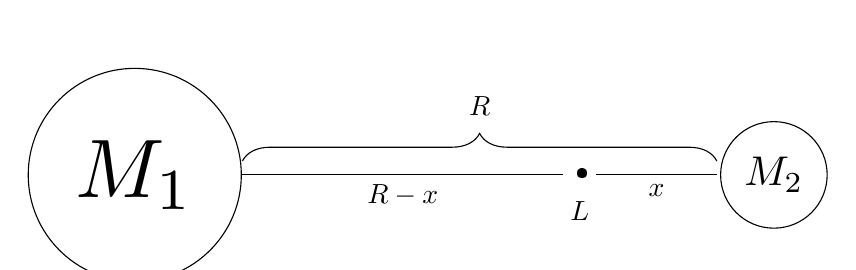
\begin{tikzpicture}[scale=\textwidth]

    %creates m1, m2, and L
    \node (m1) [circle, draw=black, fill=white, text=black,
    scale=3]{$M_1$};%draws M1
    \node (m2) [circle, draw=black, fill=white,
    text=black, scale=1.5, right=0.5\textwidth of m1]{$M_2$};%draws M2
    \node (L) [draw=white, fill=white, text=black, left=1.5 of m2]{\textbullet};%draws point L
    \node [draw=white, fill=white, text=black, below=0.01 of L]{$L$};%labels point L

    %draws lines for x and R-x
    \draw (m1) to node[midway, below, sloped]{$R-x$} (L);%draws R-x
    \draw (m2) to node[midway, below, sloped]{$x$} (L);%draws x

    %draws brace for R
    \draw [decorate, decoration={brace, amplitude=10pt, raise=5pt}] (m1) to node[midway, yshift=25pt, sloped]{$R$} (m2);%draws R (yshift is relative to line y=0)
  \end{tikzpicture}

  \caption{A diagram of two large masses $M_1$ and $M_2$ separated by distance $R$ with the lagrange point $L$ between them at the point where the force of gravity for each mass is equivalent ($F_{GM_1} = F_{GM_2}$)}
  \label{fig:lagrange_diag}
\end{figure}

%==========================
%===== Lagrange Math ======
%==========================

The Lagrange point $L$ is located at the equilibrium point for the forces of gravity for each mass. We want to find the distance of that point from the mass $M_2$.
\begin{equation*}
  F_{G,1} = F_{G,2} 
\end{equation*}

Given $F_{G,1} = F_{G,2}$, rewrite the equation for the equilibrium point. Assume the Lagrange point $L$ is $M_L$ of negligible mass.
\begin{equation*}
  G \displaystyle\frac{M_1 M_L}{r_{L,1}^2} = G\frac{M_L M_2}{r_{L,2}^2}
\end{equation*}

Replace each $r$-value with the components of $R$, those being $x$ and $R-x$, from the diagram above and cancel out shared terms as follows.
\begin{equation*}
  \displaystyle\frac{M_1}{\left(R-x\right)^2} = \frac{M_2}{x^2}
\end{equation*}

Finally, algebraically rearrange the formula to yield $x$, the distance between $L$ and $M_2$.
\begin{equation*}
  x = \frac{R}{\sqrt{\frac{m_1}{m_2}} + 1} 
\end{equation*}

\textbf{N.B.} Instruction on this material in class was especially unclear. It is advised that you perform additional research on this topic at resources like \url{http://en.wikipedia.org/wiki/Lagrangian_point} before relying on this appendix item. The authors are of the impression that the example on this page is meant for the calculation of $L_1$.

% Diagram of points <-- this might be causing the compiler to run out of time on overleaf
%\begin{figure}[p]
%  \centering
%  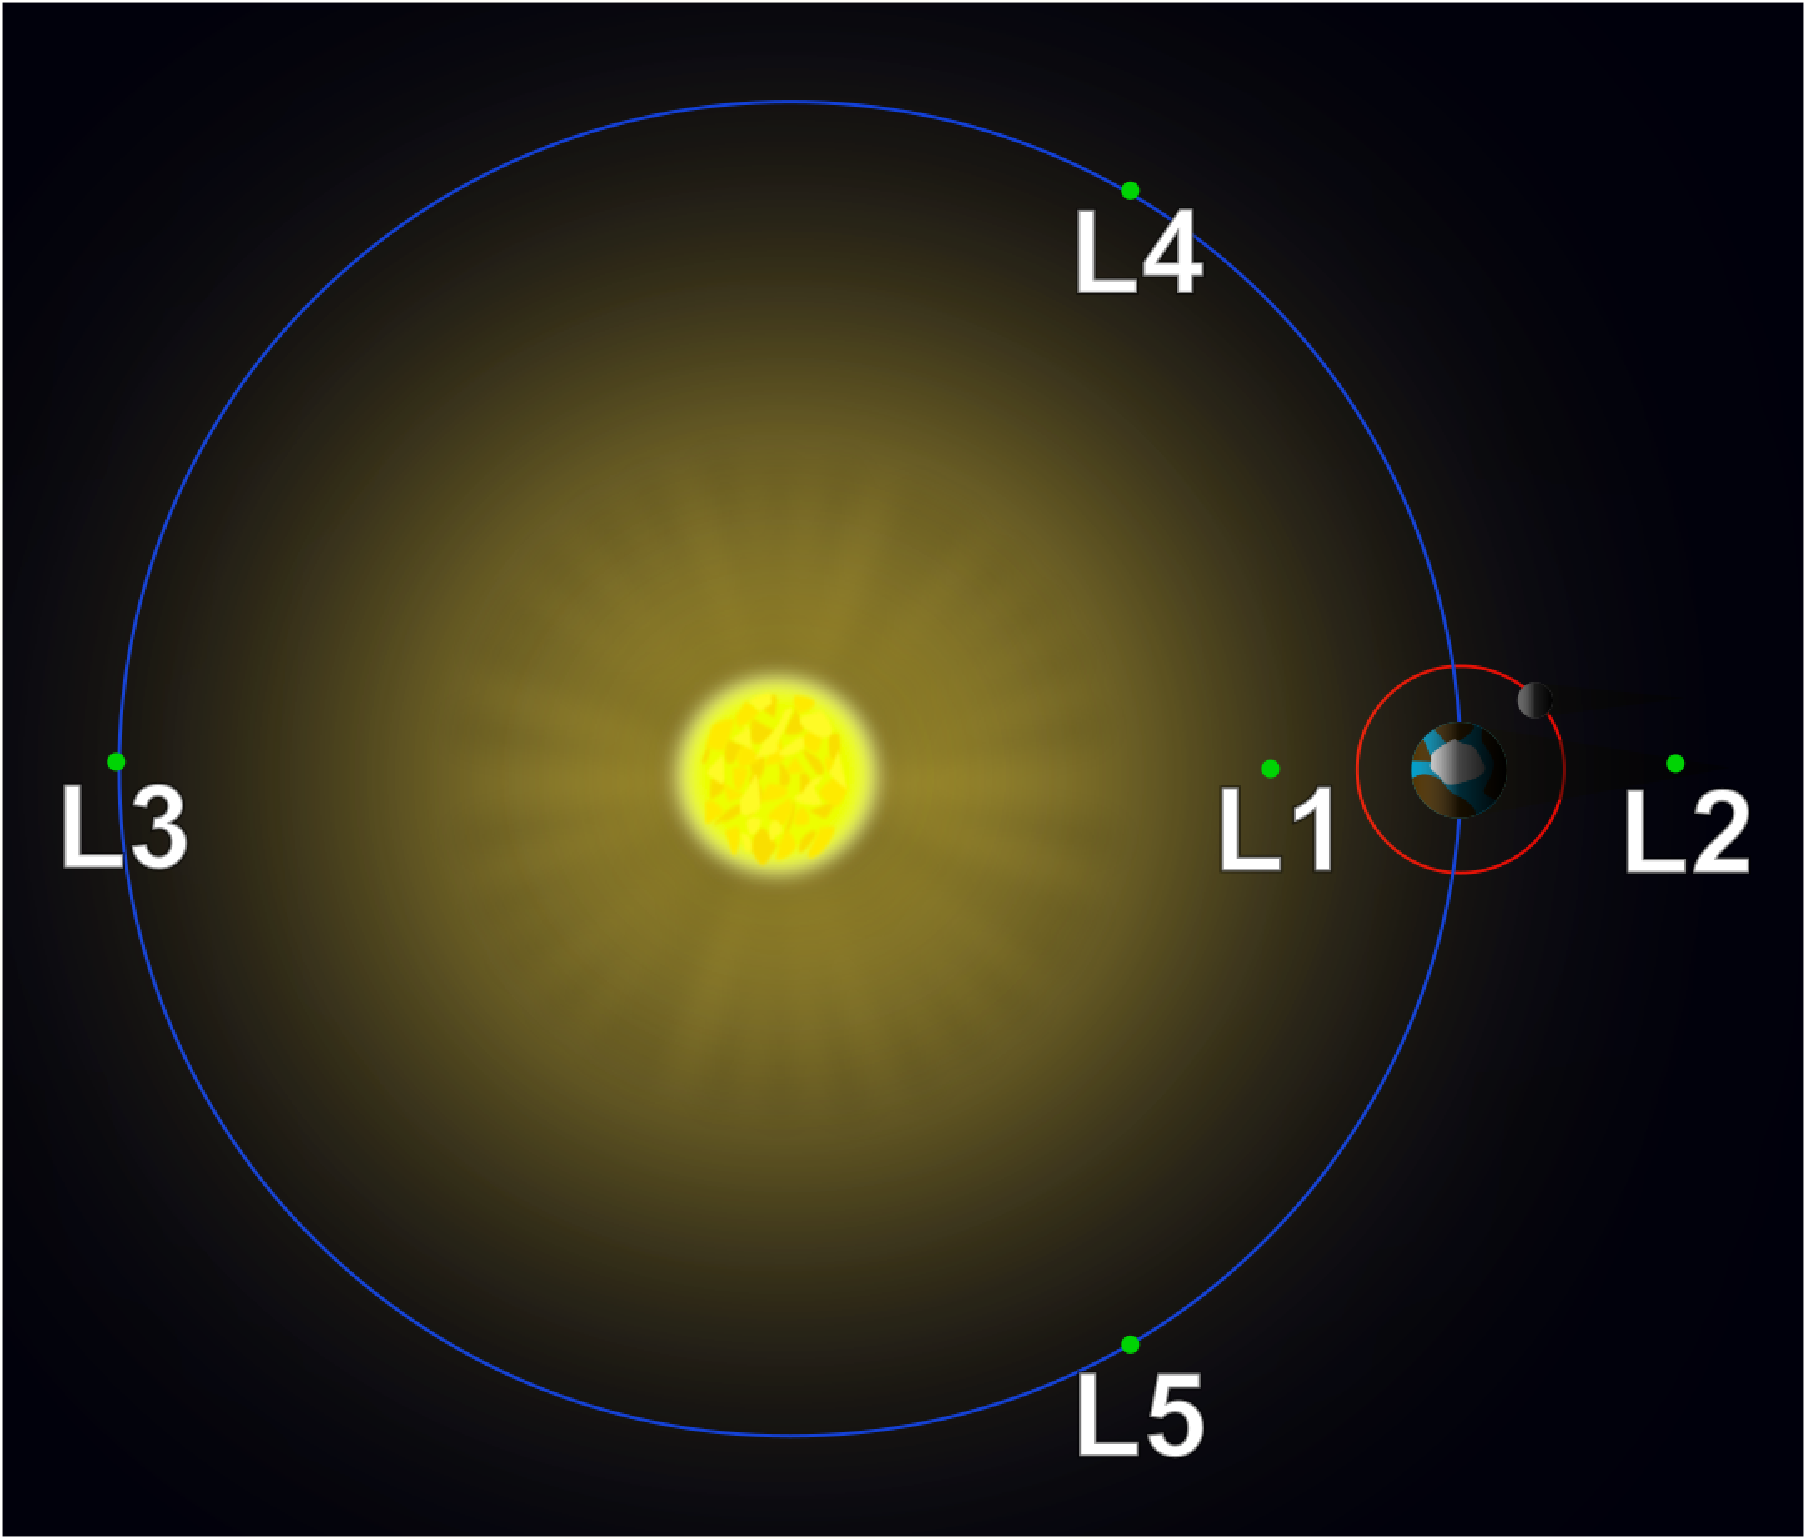
\includegraphics[width=\textwidth]{appendix-01/Lagrange_Points_Diagram} \vfill
%  \caption{A diagram of the five Langrangian points in the Moon--Earth--Sun system.}
%  \label{fig:lagrange_five}
%\end{figure}

%%% Local Variables:
%%% mode: latex
%%% TeX-master: "../main"
%%% End:
%lagrange point calculations
\clearpage\begin{longtable}{p{0.5\textwidth} p{0.5\textwidth}}
  \tablesubsection{Newton's Laws of Motion}\label{ssec:newtons-laws}
  &\\%this is for spacing of the \tablesubsection{} command
\end{longtable}

\textbf{First Law (law of inertia):}  An object at rest will remain at rest unless acted on by an unbalanced force. An object in motion continues in motion with the same speed and in the same direction unless acted upon by an unbalanced force. 

The corollary to this law is that a net force will either cause an object to leave rest or change the speed of an object.

\textbf{Second Law:} Acceleration is produced when a force acts on a mass. The greater the mass (of the object being accelerated) the greater the amount of force needed (to accelerate the object). The acceleration applied to the object is directly proportional to the net force applied, and it is inversely proportional to the mass of the object: \[ \vec{F} \propto \vec{a} \] and \[ \vec{a} \propto \frac{1}{m}. \]

Therefore, let us arrive at the following, which should be pretty familiar to you: \[ \vec{F} = m \vec{a}. \]

\textbf{Third Law:} For every action there is an equal and opposite reaction. 

Consider the rocket. The rocket's \textit{action} is to push down on the ground with the force of its powerful engines, and the \textit{reaction} is that the ground pushes the rocket upwards with an \textit{equal force}. 

For more information, visit \url{http://www.physicsclassroom.com/Physics-Tutorial/Newton-s-Laws}.
%%% Local Variables:
%%% mode: latex
%%% TeX-master: "../main"
%%% End:%a description of Newton's Laws of Motion
\clearpage\begin{longtable}{p{0.5\textwidth} p{0.5\textwidth}}
  \tablesubsection{Kepler's Laws of Planetary Motion}\label{ssec:keplers-laws}
  &\\%this is for spacing of the \tablesubsection{} command
\end{longtable}

\textbf{First Law:} All planets move in elliptical orbits with the Sun at one of the focal points.

\textbf{Second Law:} A line drawn from the Sun to any planet sweeps out equal areas in equal time intervals (i.e., velocity is maximum at perihelion and minimum at aphelion).

\textbf{Third Law:} The square of the orbital period of any planet is proportional to the cube of the average distance from that planet to the Sun, i.e. 

\begin{equation*} 
  \begin{split}
    T^2 &= K_Sr^3 \\
    T^2 &= \displaystyle\left(\frac{4\pi^2}{GM_S}\right)r^3 \\ 
    T   &= \displaystyle\sqrt{\left(\frac{4\pi^2}{GM_S}\right)r^3}.
  \end{split}
\end{equation*}

This yields the period $T$ of a planet where $M_S$ is the mass of the sun. $r$ is the average radius of the planet, and $K_S$ is a constant exactly equal to the quantity \( \displaystyle\frac{4\pi^2}{GM_S} \), or approximately \( \SI{2.97e-19}{\second\squared\per\meter\cubed} \). As a reminder, \( G \) is the universal gravitation constant approximately equal to \( \SI{6.67384e-11}{kg^{-1} m^3 s^{-2}} \).

For highly eccentric orbits, use $a$, the semi-major axis, instead. A discussion of orbital eccentricity can be found at \url{http://en.wikipedia.org/wiki/Orbital_eccentricity}. This yields 

\begin{equation*} 
  \begin{split}
    T^2 &= a^3 \\
    T &= \displaystyle\sqrt{a^3}.
  \end{split}
\end{equation*}

This equation relates the period of a body to its semi-major axis, which is measured in astronomical units (\si{\astronomicalunit}).

We may also arrive at the mass of the sun, \( M_S \), by moving around variables to arrive at

\[ M_S = \displaystyle\frac{4\pi^2}{GK_S} \approx \SI{1.989e30}{\kilogram}. \]


%%% Local Variables:
%%% mode: latex
%%% TeX-master: "../main"
%%% End:
%a description of kepler's laws of planetary motion
\clearpage\begin{longtable}{p{0.4\textwidth} p{0.6\textwidth}}
  \tablesubsection{Atwood Devices}
  \label{ssec:atwood}
  &\\%for spacing tablesubsection command
\end{longtable}

\vspace{-1cm}

\begin{center}
  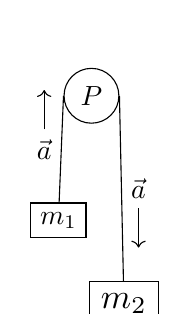
\begin{tikzpicture}
    \node (P) [circle, draw=black, fill=white, text=black, scale=1]{$P$};%draws pulley P
    \node (m1) [rectangle, draw=black, fill=white, text=black, scale=1, below=1cm of P, xshift=-0.42cm]{$m_1$};%draws m1
    \node (m2) [rectangle, draw=black, fill=white, text=black, scale=1.25, below=2cm of P, xshift=0.33cm]{$m_2$};%draws m2
    \draw (m1) to node(a1)[text=black, midway, left]{$\vec{a}$} (P.west);%connects m1 to P
    \draw (m2) to node(a2)[text=black, midway, right]{$\vec{a}$} (P.east);%connects m2 to P
    \draw[->] (a1) to +(0,0.75);%draws a1 arrow
    \draw[->] (a2) to +(0,-0.75);%draws a2 arrow
  \end{tikzpicture}
\end{center}
An Atwood device in the form of a frictionless pulley $P$ with masses $m_1$ and $m_2$ affixed to a string about the pulley with net acceleration $\vec{a}$ caused by sum of the force of gravity acting on the two masses. By convention, $m_2$ is the larger of the two masses.

\begin{longtable}{p{0.45\textwidth} p{0.45\textwidth}}
  \(\vec{T} = \left(\displaystyle\frac{2m_1m_2}{m_1+m_2}\right)g\) & Yields the force of tension acting on two objects in an Atwood device \\
  \(\vec{F}_{net} = m_2g - m_1g\) & The net force acting on the two-mass system \\
  \(\vec{a} = \displaystyle\left(\frac{m_2-m_1}{m_1+m_2}\right)g\) & The acceleration of the system relative to $m_1$ \\
\end{longtable}

\begin{center}
  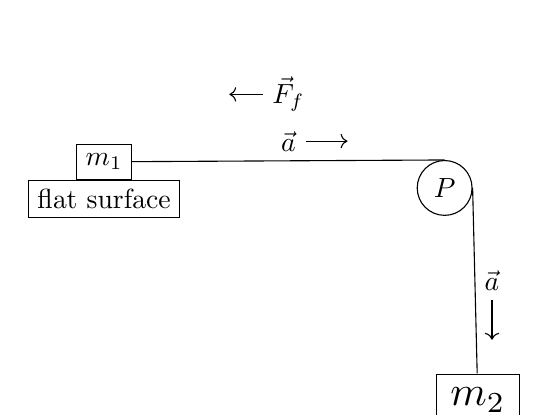
\begin{tikzpicture}
    \node (P) [circle, draw=black, fill=white, text=black, scale=1]{$P$};%draws pulley P
    \node (surf) [rectangle, draw=black, fill=white, text=black, scale=1, left=3 of P, yshift=-4]{flat surface};%draws the flat surface
    \node (m1) [rectangle, draw=black, fill=white, text=black, scale=1, above=0 of surf]{$m_1$};%draws m1 on the surface
    \draw (m1) to node(a1)[text=black, midway, above]{$\vec{a}$} (P.north);%connects m1 to P
    \node (m2) [rectangle, draw=black, fill=white, text=black, scale=1.5, below=2 of P, xshift=8]{$m_2$};%draws m2
    \draw (m2) to node(a2)[text=black, midway, right]{$\vec{a}$} (P.east);%connects m2 to P
    \draw[->] (a1) to +(0.75,0);%a1 direction
    \draw[->] (a2) to +(0,-0.75);%a2 direction
    \node (fric) [text=black, above=0 of a1]{$\vec{F}_f$};%friction
    \draw[->] (fric) to +(-0.75,0);%fric direction
  \end{tikzpicture}
\end{center}
An Atwood device in the form of a frictionless pulley $P$ where $m_1$ is placed on a horizontal surface while $m_2$ remains in free-fall. $\vec{F}_f$ is the force of friction acting on $m_1$ by the flat surface.

\begin{longtable}{p{0.45\textwidth} p{0.45\textwidth}}
  \(\vec{a} = \displaystyle\left(\frac{m_2-\mu_km_1}{m_1+m_2}\right)g\) & The acceleration of an Atwood device on a flat surface such that the effective acceleration due to gravity $\vec{a}_g$ acting upon $m_1$ is $0$ due to the restoring normal force $\vec{n}$ acting against gravity where $m_1$ is placed on a flat surface with coefficient of kinetic friction $\mu_k$ \\
\end{longtable}

\begin{center}
  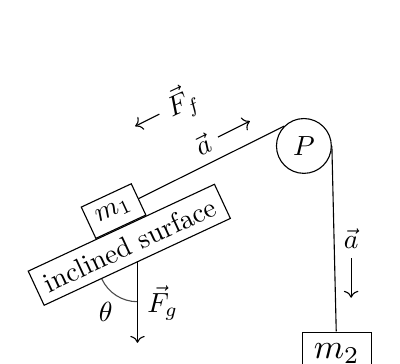
\begin{tikzpicture}
    \node (P) [circle, draw=black, fill=white, text=black, scale=1]{$P$};%draws P
    \node (surf) [rectangle, draw=black, fill=white, text=black, scale=1, rotate=25, left=1 of P, yshift=-22pt]{inclined surface};%draws surface
    \node (m1) [rectangle, draw=black, fill=white, text=black, scale=1, rotate=25, above=0 of surf]{$m_1$};%draws m1
    \draw (m1) to node(a1)[midway, above, sloped, text=black]{$\vec{a}$} (P.north west);%connects m1 to P
    \node (m2) [rectangle, draw=black, fill=white, text=black, scale=1.25, below=2cm of P, xshift=9.5pt]{$m_2$};%draws m2
    \draw (m2) to node(a2)[midway, right, text=black]{$\vec{a}$} (P.east);%connects m2 to P
    \draw[->] (a1) to +(0.6,0.3);%m1 accel
    \draw[->] (a2) to +(0,-0.75);%m2 accel
    \node (f) [text=black, scale=1, above=0 of a1, rotate=25]{$\vec{F}_f$};%friction text
    \draw[->] (f) to +(-0.6,-0.3);%friction accel
    % =============== stuff for theta ====================
    % theta nodes
    \coordinate (X) at (surf.south west){};
    \coordinate (Y) at (surf.south){};
    \coordinate (Z) at (surf.south |- 0,-2.5){};%should place Z (0,-1) relative to Y...or as close as can be, since the coordinates are being funky with this command
    % theta angle
    \tkzMarkAngle[fill=white, size=0.5cm, opacity=0.7](X,Y,Z)
    \tkzLabelAngle[pos=0.75](X,Y,Z){$\theta$}
    % theta line
    \draw[->] (Y) -- node[text=black, midway, right]{$\vec{F}_g$} (Z);
  \end{tikzpicture}
\end{center}
An Atwood device in the form of a frictionless pulley $P$ where $m_1$ is placed on an inclined surface while $m_2$ remains in free-fall. $\vec{F}_f$ is the force of friction acting on $m_1$ by the inclined surface. $\theta$ is the angle between the inclined surface and a vector in the direction of the force of gravity $\vec{F}_g$.

\begin{longtable}{p{0.45\textwidth} p{0.45\textwidth}}
  \(\vec{a} = \displaystyle\left(\frac{m_2 - m_1 \sin\theta}{m_1 + m_2}\right)g\) & The acceleration of an Atwood device on an inclined flat surface, neglecting friction \\
  \(\vec{a} = \displaystyle\left(\frac{m_2-\left(m_1\sin\theta + \mu_km_1\sin\theta \right)}{m_1 + m_2}\right)g\) & The acceleration of an Atwood device on an inclined flat surface, respecting friction between $m_1$ and the inclined surface, but neglecting friction of pulley $P$
\end{longtable}

% 
% POST-DIAGRAM ATWOOD STUFF
% 

For very small mass differences between $m_1$ and $m_2$, the rotational inertia $I$ of any pulley $P$ of radius $r$ cannot be neglected. The angular acceleration of the pulley is given by the no-slip condition:

\begin{longtable}{p{0.45\textwidth} p{0.45\textwidth}}
  \( \displaystyle\vec{\alpha} = \frac{\vec{a}}{r} \) & Yields the angular acceleration $\vec{\alpha}$ \\
  \(\displaystyle\vec{\tau}_{net}=\left(\vec{T}_1 - \vec{T}_2 \right)r - \vec{\tau}_f = I \vec{\alpha} \) & Yields the net torque $\vec{tau}_{net}$ where $\vec{\tau}_f$ is the torque due to friction and $\Delta\vec{T}$ is the difference in tensions $\vec{T}_1$ and $\vec{T}_2$ due to $m_1$ and $m_2$ \\
\end{longtable}

Combining Newton's second law for the hanging masses and solving for $\vec{T}_1$, $\vec{T}_2$, and $\vec{a}$, we get:

\begin{longtable}{p{0.45\textwidth} p{0.45\textwidth}}
  \( \displaystyle \vec{a} = \frac{g \left(m_1 - m_2 \right) - \left( \frac{\vec{\tau}_f}{r} \right)}{m_1 + m_2 + \left(\frac{I}{r^2} \right)}\) & Yields the acceleration of the Atwood system \\
  \(\displaystyle \vec{T}_1 = \frac{m_1 g \left(2 m_2 + \frac{I}{r^2} + \frac{\vec{\tau}_f}{r g} \right)}{m_1 + m_2 + \left(\frac{I}{r^2} \right)}\) & Tension in the string segment nearest $m_1$ \\
  \(\displaystyle \vec{T}_2 = \frac{m_2 g \left(2 m_1 + \frac{I}{r^2} + \frac{\vec{\tau}_f}{r g}\right)}{m_1 + m_2 + \left(\frac{I}{r^2}\right)} \) & Tension in the string segment nearest $m_2$
\end{longtable}

Should bearing friction be negligible (but not the inertia of the pulley and not the traction of the string on the pulley rim), the equations simplify as the following results:

\begin{longtable}{p{0.3\textwidth} p{0.3\textwidth} p{0.3\textwidth}}
  \( \displaystyle \vec{a} = \frac{g \left(m_1 - m_2 \right)}{m_1 + m_2 + \frac{I}{r^2}} \) & \( \displaystyle \vec{T}_1 = \frac{m_1 g \left(2 m_2 + \frac{I}{r^2} \right)}{m_1 + m_2 + \frac{I}{r^2}} \) & \( \displaystyle \vec{T}_2 = \frac{m_2 g \left(2 m_1 + \frac{I}{r^2} \right)}{m_1 + m_2 + \frac{I}{r^2}} \) \\
\end{longtable}

These examples provide but some of the many Atwood device situations you may encounter in your journey through the world of physics.

%%% Local Variables:
%%% mode: latex
%%% TeX-master: "../main"
%%% End:%atwood device calculations
\clearpage\begin{tabular}{p{0.5\textwidth} p{0.5\textwidth}}
  \tablesubsection{Work Done by a Varying Force}
  \label{ssec:varying_force_work}
   & \\%adds spacing stuff
\end{tabular}

\pgfplotsset{%DEFINES INTEGRAL STUFF
  integral segments/.code={\pgfmathsetmacro\integralsegments{#1}},
  integral segments=40,%modify to adjust number of rectangles
  integral/.style args={#1:#2}{
    ybar interval,
    domain=#1+((#2-#1)/\integralsegments)/2:#2+((#2-#1)/\integralsegments)/2,
    samples=\integralsegments+1,
    x filter/.code=\pgfmathparse{\pgfmathresult-((#2-#1)/\integralsegments)/2}
  }
}

\begin{center}
  \begin{tikzpicture}
    \begin{axis}[
      xlabel=$x$,
      ylabel=$F_x$,
      xtick={0,1,2,3,4,5,6},
      ytick={0,2,4,6,8,10},
      xmax=6, ymax=10, ymin=0, xmin=0,
      enlargelimits=true,
      axis lines=left,
      clip=false,
      domain=0:6,
      axis on top
      ]

      \addplot[mark=none, color=blue, thick]{-(x-3)^2+9}\closedcycle;%formula to represent integral
      \addplot[integral=0:6]{-(x-3)^2+9};
    \end{axis}
  \end{tikzpicture}
\end{center}  

The above is a graph of the varying force $F_x$ across a distance $x$ with Riemann sums approximating its integral. Each rectangle has a length equal to the magnitude of $F_x$ and a width equal to the small distance $x_i$. \\

%VARYING FORCE MATH

The following formula yields the work done by a varying force $F_x$ described above. In this formula, $F_i$ is the magnitude of the varying force $F_x$ at the midpoint of a small distance $\Delta x_i$, the width of one of a number of infinitely small rectangles whose area may be approximated $A = \ell w = F_i\Delta x_i$.

\[ W \cong \sum_{i=1}^{\infty} F_i \Delta x_i \]

The definite integral found below is an alternate representation of the above Riemann sum, approximating the work performed by a force $F_x$ at each point $x$ across the distance $\Delta x = x_f - x_i$.

\[ \int_{x_i}^{x_f} F_x \]
%%% Local Variables:
%%% mode: latex
%%% TeX-master: "../main"
%%% End:%varying force work calculations
\clearpage\begin{tabular}{p{0.5\textwidth} p{0.5\textwidth}}
  \tablesubsection{Work Done by a Constant Force}
   & \\%adds spacing stuff
\end{tabular}

%commands for positioning the triangle
\newcommand{\triht}{5cm}
\newcommand{\triwd}{7cm}

\newcommand{\dispht}{1cm}
\newcommand{\dispwd}{10cm}

% http://tex.stackexchange.com/questions/166958/draw-with-tikz-a-pythagorean-triangle-with-the-squares-of-its-sides-and-labels
% http://tex.stackexchange.com/questions/96459/automatically-draw-and-labels-angles-of-a-triangle-in-tikz

\begin{center}
  \begin{tikzpicture}%[thick]
    \coordinate (A) at (0,0);
    \coordinate (B) at (0+\triwd,0);
    \coordinate (C) at (0+\triwd,0+\triht);

    \draw [->] (A)--(B);
    \draw [dashed, ->] (B)--(C);
    \draw [ultra thick, ->] (A)--(C);

    \tkzLabelSegment[below=2pt](A,B){${F}{\cos\theta}$}
    \tkzLabelSegment[left=2pt](A,C){$\vec{F}$}
    \tkzLabelSegment[above right=2pt](B,C){$\cancel{{F}{\sin\theta}}$}

    % \tkzMarkRightAngle[fill=orange,size=0.5,opacity=.4](A,B,C)% square angle here
    % \tkzLabelAngle[pos = 0.35](A,B,C){$\gamma$}

    \tkzMarkAngle[fill= blue,size=1.5cm,opacity=.4](B,A,C)
    \tkzLabelAngle[pos = 0.75](B,A,C){$\theta$}

    % \tkzMarkAngle[fill= orange,size=0.7cm,opacity=.4](A,C,B)
    % \tkzLabelAngle[pos = 0.5](A,C,B){$\beta$}

    \coordinate (Xi) at (0,-\dispht);
    \coordinate (Xf) at (\dispwd,-\dispht);

    \coordinate (Xi_bar1) at (0,-\dispht-0.25cm);
    \coordinate (Xf_bar1) at (\dispwd,-\dispht-0.25cm);
    \coordinate (Xi_bar2) at (0,0);
    \coordinate (Xf_bar2) at (\dispwd,0);


    \draw [ultra thick, ->] (Xi)--(Xf);
    \tkzLabelSegment[below=2pt](Xi,Xf){$\Delta \vec{x}$}
    % \draw [o] (0,-\dispht);

    \draw (Xi_bar1)--(Xi_bar2);
    \draw (Xf_bar1)--(Xf_bar2);

  \end{tikzpicture}
\end{center}

A constant force $\vec{F}$ exerted at an angle $\theta$ with respect to the displacement, $\Delta\vec{x}$, performs work \(\displaystyle W = ({F}{\cos\theta}){\Delta x}\).
%%% Local Variables:
%%% mode: latex
%%% TeX-master: "../main"
%%% End:
%constant force work diagram
\clearpage\begin{tabular}{p{0.5\textwidth} p{0.5\textwidth}}
  \tablesubsection{Miscellaneous Angular Formul\ae}\label{ssec:angular-formulae}
  
  \(\vec{\omega} = 2\pi f\) & The quantity $\vec{\omega}$ is alternatively termed the angular frequency. A frequency $f$ is stated typically in Hertz (\si{\hertz}) but also common is revolutions per minute or second, rotations per minute and cycles per minute/second (these are all essentially equivalent terminology) \\
  \(fT=1\) & Frequency $f$ and period $T$ are inversely related. Frequency is typically measured in \si{\hertz} while period is measured in \si{\second} \\

  \notabene{One radian is the angle subtended at the centre of a circle by an arc equal in length to the radius of the circle. Thus, an angle $\theta$ in radians is given in terms of the arc length $\ell$ it subtends on a circle of radius $r$ by the equation $\theta=\frac{\ell}{r}$. Furthermore, \(\SI{1}{\revolution}=\SI{360}{\degree}=\SI{2\pi}{\radian}\)}
  \notabene{When converting from \textit{Degrees} to \textit{Radians}, use \(x\textrm{\space}\si{\degree}\times\frac{\pi}{180}\). When converting from \textit{Radians} to \textit{Degrees}, use \(x\textrm{\space}\si{\radian}\times\frac{180}{\pi}\)}
  \notabene{When converting from \textit{Revolutions per Minute} to \textit{Radians per Second}, use \(x\textrm{\space}\si{\revolution\per\minute}\times\frac{2\pi}{60}\si{\radian\per\second}\)}
\end{tabular}
%%% Local Variables:
%%% mode: latex
%%% TeX-master: "../main"
%%% End:%miscellaneous angular formulae
\clearpage\begin{longtable}{p{0.5\textwidth} p{0.5\textwidth}}
  \tablesubsection{Mach Number \& Shock Waves}
   & \\
\end{longtable}
\begin{figure}[h]
  \centering
  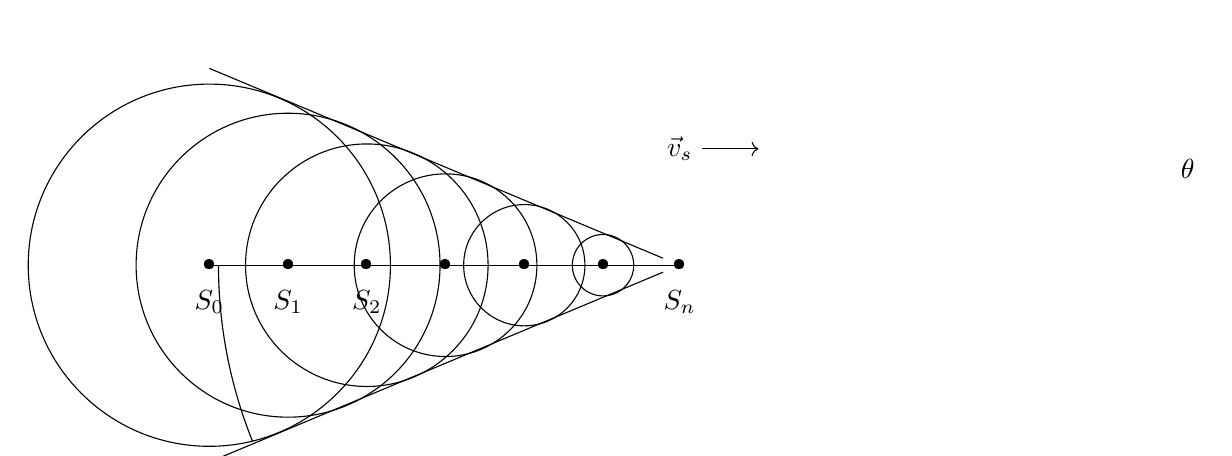
\begin{tikzpicture}
    %draws the circles with labels and v_s
    \draw (0,0) circle [radius=2.3] node (s0) [text=black] {\textbullet} node [text=black, below=0 of s0] {$S_0$};
    \draw (1,0) circle [radius=1.93] node (s1) [text=black] {\textbullet} node [text=black, below=0 of s1] {$S_1$};
    \draw (2,0) circle [radius=1.54] node (s2) [text=black] {\textbullet} node [text=black, below=0 of s2] {$S_2$};
    \draw (3,0) circle [radius=1.16] node (s3) [text=black] {\textbullet};
    \draw (4,0) circle [radius=0.77] node (s4) [text=black] {\textbullet};
    \draw (5,0) circle [radius=0.39] node (s5) [text=black] {\textbullet};
    \node (sn) [text=black, right=0.55 of s5] {\textbullet} node [text=black, below=0 of sn] {$S_n$};
    \node (vs) [text=black, above=1 of sn] {$\vec{v}_s$};
    \draw [->] (vs) to +(1,0);
    %draws the three lines
    \draw (0,0) -- (6,0);%line from s0 to sn
    \draw (sn) to (s0 |- 0,2.5);%top line
    \draw (sn) to (s0 |- 0,-2.5);%bottom line
    %labels the angle
    \node (endpoint) [below=2.13 of s0]{};%angle endpoint
    \node (midpoint) [right=0.78 of s5]{};%angle midpoint
    \tkzMarkAngle[fill=none, size=6cm,opacity=1](s0,midpoint,endpoint);%to make the line at the end
    \tkzMarkAngle[fill=blue, size=6cm, opacity=0.1](s0,midpoint,endpoint);%to fill the angle without touching the line at the end
    \tkzLabelAngle[pos=-7.5](s0,midpoint,endpoint){$\theta$};
  \end{tikzpicture}
  \caption{A representation of a shock wave, produced when a source moves from $S_0$ to $S_n$ with a speed $\vec{v}_s$ which is greater than the wave speed $\vec{v}$ in the medium where the radius of each circle surrounding a point $S_x$ is $\vec{v}t$, the velocity $\vec{v}$ of sound in the medium multiplied by $t$, the amount of time elapsed since the source of the sound was at a point $S_x$}
  \label{fig:shock-waves}
\end{figure}
\begin{longtable}{p{0.5\textwidth} p{0.5\textwidth}}
  \(\displaystyle\sin\theta=\frac{\vec{v}}{\vec{v}_s} \therefore \theta=\arcsin\left(\frac{\vec{v}}{\vec{v}_s}\right)\) & Yields the angle $\theta$ between a line tangent to a circle and the direction of motion of the sound source where $\vec{v}$ is the speed of sound in a that medium and $\vec{v}_s$ is the velocity of the sound source in that medium \\

  \notabene{The ratio $\frac{\vec{v}}{\vec{v}_s}$ is the \textit{Mach number}. The conical wave front produced when $\vec{v}_s > \vec{v}$ (supersonic speeds) is known as a shock wave. An interesting example of a shock wave is the bow wave of a boat when the boat's speed exceeds the speed of the water waves}
\end{longtable}
%%% Local Variables:
%%% mode: latex
%%% TeX-master: "../main"
%%% End:%mach number & shock wave calculations
\clearpage\begin{longtable}{p{0.5\textwidth} p{0.5\textwidth}}
  \tablesubsection{Beat Frequency}
   & \\
\end{longtable}
\begin{figure}[h!]
  \centering
  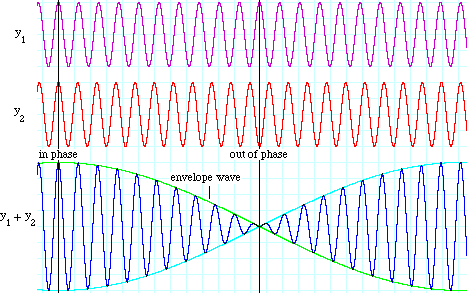
\includegraphics[scale=1]{appendix-01/beat-frequency-image}
  \caption{A diagram of the beat frequency between the waves $y_1$ and $y_2$ as traveling in the same direction where the beat frequency $f_b=\abs{f_2-f_1}$. The nodes of the combined wave occur where $y_1$ and $y_2$ are out of phase|that is, they have opposite amplitudes---and the antinodes of the combined wave occur where $y_1$ and $y_2$ are in phase---that is, they have equal amplitudes}
  \label{fig:beat-frequency}
\end{figure}
%%% Local Variables:
%%% mode: latex
%%% TeX-master: "../main"
%%% End:
%beat frequency stuff
%NOTE: cannot nest \include{} statements, that's why everything is using \clearpage\input{} instead
%%% Local Variables:
%%% mode: latex
%%% TeX-master: "../main"
%%% End:
%app.01: supplementary information
%NOTE: header information stored in constant-reference.tex
\begin{longtable}{p{0.5\textwidth} p{0.5\textwidth}}
  \tablesection{Appendix II: Quick Reference Information}
  \tablesubsection{Physical Constants}
  & \\%needed for formatting
\end{longtable}
\vspace{-1cm}
\begin{longtable}{l c c c}
  Quantity & Symbol & Value & SI Unit \\
  \midrule
  Avogadro's Number & \(N_A\) & $6.02\e{23}$ & \si{particles\per\mole} \\
  Bohr radius & $a_0$ & $5.29\e{-11}$ & \si{\meter} \\
  Boltzmann's constant & $k_B$ & $1.38\e{-23}$ & \si{\joule\per\kelvin} \\
  Coulomb Constant, $\frac{1}{4\pi\epsilon_0}$ & $k_e$ & $8.99\e{9}$ & \si{\newton\meter\squared\per\coulomb\squared} \\
  Electron Compton wavelength & $\frac{h}{m_ec}$ & $2.43\e{-12}$ & \si{\meter} \\
  Electron mass & $m_e$ & $9.11\e{-31}$ & \si{\kilo\gram} \\
           && $5.49\e{-4}$ & \si{\atomicmassunit} \\
           && \SI{0.511}{\mega\electronvolt\per\lightspeed\squared}& \\
  Elementary charge & $e$ & $1.60\e{-19}$ & \si{\coulomb} \\
  Gravitational constant & $G$ & $6.67\e{-11}$ & \si{\newton\meter\squared\per\kilo\gram\squared} \\
  Mass of Earth & $M_E$ & $5.98\e{24}$ & \si{\kilo\gram} \\
  Mass of Moon & $M_M$ & $7.36\e{22}$ & \si{\kilo\gram} \\
  Molar volume of ideal gas at STP & $V$ & 22.4 & \si{\liter\per\mole} \\
           && $2.24\e{-2}$ & \si{\meter\cubed\per\mole} \\
  Neutron mass & $m_n$ & $1.67493\e{-27}$ & \si{\kilo\gram} \\
           && 1.008665 & \si{\atomicmassunit} \\
           && \SI{939.565}{\mega\electronvolt\per\lightspeed\squared}& \\
  Permeability of free space & $\mu_0$ & $1.26\e{-6}$ & \si{\meter\kilo\gram\per\second\squared\per\ampere\squared} \\
           && $\left(4\pi\e{-7}\textrm{\space exactly}\right)$&\\
  Permittivity of free space & $\epsilon_0$ & $8.85\e{-12}$ & \si{\coulomb\squared\per\newton\per\meter\squared} \\
  Planck's constant & $h$ & $6.63\e{-34}$ & \si{\joule\second} \\
           & $\hslash=\frac{h}{2\pi}$ & $1.05\e{-34}$ & \si{\joule\second} \\
  Proton mass & $m_p$ & $1.67262\e{-27}$ & \si{\kilo\gram} \\
           && 1.007276 & \si{\atomicmassunit} \\
  Radius of Earth (at equator) & $R_E$ & $6.38\e{6}$ & \si{\meter} \\
  Radius of Moon & $R_M$ & $1.74\e{6}$ & \si{\meter} \\
  Rydberg constant & $R_H$ & $1.10\e{7}$ & \si{\meter^{-1}} \\
  Speed of light in vacuum & $c$ & $3.00\e{8}$ & \si{\meter\per\second} \\
  Standard free-fall acceleration & $g$ & 9.80 & \si{\meter\per\second\squared} \\
  Stefan-Boltzmann constant & $\sigma$ & $5.67\e{-8}$ & \si{\watt\per\meter\squared\per\kelvin^4} \\
  Universal gas constant & $R$ & 8.31 & \si{\joule\per\mole\per\kelvin} \\
  \bottomrule
\end{longtable}


%%% Local Variables:
%%% mode: latex
%%% TeX-master: "../main"
%%% End:
%reference sheet for constants
\vspace{1cm}\begin{tabular}{p{0.5\textwidth} p{0.5\textwidth}}
  \tablesubsection{Masses for selected Subatomic Particles}
  \label{ssec:atomic-mass}
  &\\%spacing stuff out
\end{tabular}

\begin{center}%centers the table
  \begin{tabular}{l c c c}
    \textbf{Particle} & \textbf{\si{\kilo\gram}} & \textbf{\si{\atomicmassunit}} & \textbf{\si{\mega\electronvolt\per\lightspeed\squared}} \\
    \hline
    Proton & $1.6726\e{-27}$ & $1.007276$ & $938.28$ \\
    Neutron & $1.6750\e{-27}$ & $1.008665$ & $939.57$ \\
    Electron & $9.109\e{-31}$ & $5.486\e{-4}$ & $0.511$ \\
  \end{tabular}
\end{center}

%%% Local Variables:
%%% mode: latex
%%% TeX-master: "../main"
%%% End:
%subatomic particle (e.g., proton) mass data
\clearpage\begin{longtable}{p{0.5\textwidth} p{0.5\textwidth}}
  \tablesubsection{Unit Conversion Factors}  

  \textbf{Length} & \textbf{Speed} \\
  \(\SI{1}{\meter}=\SI{39.37}{\inch}=\SI{3.281}{\foot}\) & \(\SI{1}{\kilo\meter\per\hour}=\SI{0.278}{\meter\per\second}=\SI{0.621}{\mile\per\hour}\) \\
  \(\SI{1}{\inch}=\SI{2.54}{\centi\meter}\,\textrm{(exact)}\) & \(\SI{1}{\meter\per\second}=\SI{2.237}{\mile\per\hour}=\SI{3.281}{\foot\per\second}\) \\
  \(\SI{1}{\kilo\meter}=\SI{0.621}{\mile}\) & \(\SI{1}{\mile\per\hour}=\SI{1.61}{\kilo\meter\per\hour}=\SI{0.447}{\meter\per\second}=\SI{1.47}{\foot\per\second}\) \\
  \(\SI{1}{\mile}=\SI{5280}{\foot}=\SI{1.609}{\kilo\meter}\) & \textbf{Force} \\
  \(\SI{1}{\lightyear}\,\textrm{(lightyear)}=9.461\e{15}\,\si{\meter}\) & \(\SI{1}{\newton}=\SI{0.2248}{\pound}=10^5\si{\dyne}\,\textrm{(dyne)}\) \\
  \(\SI{1}{\angstrom}\,\textrm{(\"angstr\"om)}=10^{-10}\,\si{\meter}\) & \(\SI{1}{\pound}=\SI{4.448}{\newton}\) \\
  \textbf{Mass} & \(\SI{1}{\dyne}=10^{-5}\,\si{\newton}=2.248\e{-6}\,\si{\pound}\) \\
  \(\SI{1}{\kilo\gram}=10^3\,\si{\gram}=6.85\e{-2}\,\si{\slug}\) & \textbf{Work \& Energy} \\
  \(\SI{1}{\slug}=\SI{14.59}{\kilo\gram}\) & \(\SI{1}{\joule}=10^7\,\si{\ergon}\,\textrm{(ergon)}=\SI{0.738}{\foot\pound}=\SI{0.239}{\calorie}\) \\
  \(\SI{1}{\atomicmassunit}=1.66\e{-27}\,\si{\kilo\gram}=\SI{931.5}{\mega\electronvolt\per\lightspeed\squared}\) & \(\SI{1}{\calorie}=\SI{4.186}{\joule}\) \\
  \textbf{Time} & \(\SI{1}{\foot\pound}=\SI{1.356}{\joule}\) \\
  \(\SI{1}{\minute}=\SI{60}{\second}\) & \(\SI{1}{\britishthermalunit}=1.054\e{3}\,\si{\joule}=\SI{252}{\calorie}\) \\
  \(\SI{1}{\hour}=\SI{3600}{\second}\) & \(\SI{1}{\joule}=6.24\e{18}\,\si{\electronvolt}\) \\
  \(\SI{1}{\day}=\SI{24}{\hour}=1.44\e{3}\,\si{\minute}=8.64\e{4}\,\si{\second}\) & \(\SI{1}{\electronvolt}=1.602\e{-19}\,\si{\joule}\) \\
  \(\SI{1}{\year}=\SI{365.242}{\day}=3.156\e{7}\,\si{\second}\) & \(\SI{1}{\kilo\watt\hour}=3.60\e{6}\,\si{\joule}\) \\
  \textbf{Volume} & \textbf{Pressure} \\
  \(\SI{1}{\liter}=\SI{1000}{\centi\meter\cubed}=\SI{0.0353}{\foot\cubed}\) & \(\SI{1}{\atmosphere}=1.013\e{5}\,\si{\newton\per\meter\squared}=\SI{14.70}{\pound\per\inch\squared}\) \\
  \(\SI{1}{\foot\cubed}=2.832\e{-2}\,\si{\meter\cubed}\) & \(\SI{1}{\pascal}=\SI{1}{\newton\per\meter\squared}=1.45\e{-4}\,\si{\pound\per\inch\squared}\) \\
  \(\SI{1}{\gallon}=\SI{3.786}{\liter}=\SI{231}{\inch\cubed}\) & \(\SI{1}{\pound\per\inch\squared}=6.895\e{3}\,\si{\newton\per\meter\squared}\) \\
  \textbf{Angle} & \textbf{Power} \\
  \(\SI{180}{\degree}=\SI{\pi}{\radian}\,\textrm{(radian)}\) & \(\SI{1}{\horsepower}\,\textrm{(horsepower)}=\SI{550}{\foot\pound\per\second}=\SI{0.746}{\kilo\watt}\) \\
  \(\SI{1}{\radian}=\SI{57.30}{\degree}\) & \(\SI{1}{\watt}=\SI{1}{\joule\per\second}=\SI{0.738}{\foot\pound\per\second}\) \\
  \(\SI{1}{\degree}=\SI{60}{\minute}=1.745\e{-2}\,\si{\radian}\) & \(\SI{1}{\britishthermalunit\per\hour}=\SI{0.293}{\watt}\) \\
\end{longtable}
%%% Local Variables:
%%% mode: latex
%%% TeX-master: "../main"
%%% End:
%unit conversions reference
\clearpage\begin{longtable}{p{0.6\textwidth} p{0.15\textwidth} p{0.15\textwidth}}
  \cmidrule(r){1-3}\multicolumn{3}{c}{The Greek Alphabet}\addcontentsline{toc}{subsection}{The Greek Alphabet}\label{ssec:greek-alphabet}\\\cmidrule(r){1-3}%adapted from \tablesubsection for 3-column table
&&\\%spacing stuff out
  \multicolumn{3}{c}{
  \begin{tabular}{l c c}
    Extended Name & Uppercase & Lowercase \\ 
    \midrule
    Alpha & A & $\alpha$ \\
    Beta & B & $\beta$ \\
    Gamma & $\Gamma$ & $\gamma$ \\
    Delta & $\Delta$ & $\delta$ \\
    Epsilon & E & $\epsilon$ \\
    Zeta & Z & $\zeta$ \\
    Eta & H & $\eta$ \\
    Theta & $\Theta$ & $\theta$ \\
    Iota & I & $\iota$ \\
    Kappa & K & $\kappa$ \\
    Lambda & $\Lambda$ & $\lambda$ \\
    Mu & M & $\mu$ \\
    Nu & N & $\nu$ \\
    Xi & $\Xi$ & $\xi$ \\
    Omicron & O & o \\
    Pi & $\Pi$ & $\pi$ \\
    Rho & P & $\rho$ \\
    Sigma & $\Sigma$ & $\sigma$ \\
    Tau & T & $\tau$ \\
    Upsilon & $\Upsilon$ & $\upsilon$ \\
    Phi & $\Phi$ & $\phi$ \\
    Chi & X & $\chi$ \\
    Psi & $\Psi$ & $\psi$ \\
    Omega & $\Omega$ & $\omega$ \\
    \bottomrule
  \end{tabular}
  }
\end{longtable}
%%% Local Variables:
%%% mode: latex
%%% TeX-master: "../main"
%%% End:
%lookup table for greek characters
\clearpage\begin{longtable}{p{0.5\textwidth} p{0.5\textwidth}}
  \tablesubsection{Selected Coefficients of Static and Kinetic Friction}
  \label{ssec:coef-fric}
  &\\
\end{longtable}

\begin{center}%centers the table
\begin{tabular}{l c c}
  Materials	Involved & ${\mu}_{s}$ & ${\mu}_{k}$ \\
  \midrule
  Steel on Steel & 0.74 & 0.57\\
  Aluminum on Steel & 0.61 & 0.47\\
  Copper on Steel & 0.53 & 0.36\\
  Rubber on Concrete & 1.0 & 0.8\\
  Wood on Wood & 0.25--0.5 & 0.2\\
  Glass on Glass & 0.94	& 0.4\\
  Waxed wood on Wet snow & 0.14	& 0.1\\
  Waxed wood on Dry snow & --- & 0.04\\
  Metal on Metal (lubricated) & 0.15 & 0.06\\
  Ice on Ice & 0.1 & 0.03\\
  Teflon on Teflon & 0.04 & 0.04\\
  Synovial joints in humans & 0.01 & 0.003\\
  \bottomrule
\end{tabular}
\end{center}

Some coefficients of static and kinetic friction for various materials, where ${\mu}_{s}$ represents the coefficient of static friction and ${\mu}_{k}$ represents the coefficient of kinetic friction.
%%% Local Variables:
%%% mode: latex
%%% TeX-master: "../main"
%%% End:
%coefficients of friction table
\vspace{1cm}\begin{longtable}{p{0.5\textwidth} p{0.5\textwidth}}			
  \tablesubsection{Moment of Inertia Formul\ae}
  \label{ssec:moment-inertia}\\
&\\%needed for spacing
\end{longtable}	
\vspace{-2cm}
\begin{tabular}{l l l}
  Particle: \( I = mr^2 \) & Annular cylinder: \( \displaystyle I = \frac{1}{2}{m}({r_1^2 + r_2^2}) \) & Thin rod (middle): \( \displaystyle I = \frac{1}{12}{m}{r^2} \) \\ 
  Solid sphere: \( \displaystyle I = \frac{2}{5}{m}{r^2} \) & Thin rod (end): \( \displaystyle I = \frac{1}{3}{m}{L^2} \) & Hollow sphere; \( \displaystyle I = \frac{2}{3}{m}{r^2} \) \\
  Hoop or ring: \( I = mr^2 \) & Rectangular plate: \( \displaystyle I = \frac{1}{12}{m}(a^2 + b^2) \) & Cylinder or disk; \( \displaystyle I = \frac{1}{2}{m}{r^2} \) \\
  Thin sheets: see thin rods & & \\
  \bottomrule
\end{tabular}

A table of moments of inertia $I$ for several various shapes. Applications usually are found for torque equations of the form \( \tau = I \alpha \). The moment of inertia is the rotational analogue to mass.
%%% Local Variables:
%%% mode: latex
%%% TeX-master: "../main"
%%% End:

%moments of inertia
\clearpage\begin{longtable}{p{0.5\textwidth} p{0.5\textwidth}}
  \tablesubsection{Planetary Data}
  \label{ssec:plan-data}\\
&\\%spacing stuff out
\end{longtable}
\begin{figure}[h]
  \centering
  \begin{tabular}{l r c c c r}
    & Mass (\si{\kilo\gram}) & Mean Radius (\si{\meter}) & Period (\si{\second}) & Distance from Sun (\si{\meter}) & ${\displaystyle\frac{T^2}{r^3}}\left(\si{\second\squared\per\meter\cubed}\right)$ \\
    \midrule
    Mercury & 3.18\e{23} & 2.43\e{6} & 7.60\e{6} & 5.79\e{10} & 2.97\e{-19} \\
    Venus & 4.88\e{24} & 6.06\e{6} & 1.94\e{7} & 1.08\e{11} & 2.99\e{-19} \\
    Earth & 5.98\e{24} & 6.37\e{6} & 3.156\e{7} & 1.496\e{11} & 2.97\e{-19} \\
    Mars & 6.42\e{23} & 3.37\e{6} & 5.94\e{7} & 2.28\e{11} & 2.98\e{-19} \\
    Jupiter & 1.90\e{27} & 6.99\e{7} & 3.74\e{8} & 7.78\e{11} & 2.97\e{-19} \\
    Saturn & 5.68\e{26} & 5.85\e{7} & 9.35\e{8} & 1.43\e{12} & 2.99\e{-19} \\
    Uranus & 8.68\e{25} & 2.33\e{7} & 2.64\e{9} & 2.87\e{12} & 2.95\e{-19} \\
    Neptune & 1.03\e{26} & 2.21\e{7} & 5.22\e{9} & 4.50\e{12} & 2.99\e{-19} \\ 
    Pluto & $\sim$1.4\e{22} & $\sim$1.5\e{6} & 7.82\e{9} & 5.91\e{12} & 2.96\e{-19} \\
    Moon & 7.36\e{22} & 1.74\e{6} & --- & --- & --- \\ 
    Sun & 1.991\e{30} & 6.96\e{8} & --- & --- & --- \\
    \bottomrule
  \end{tabular}
\end{figure}
A table of planetary data most relevant to application with Kepler's Laws of Planetary Motion
%%% Local Variables:
%%% mode: latex
%%% TeX-master: "../main"
%%% End:
%planetary data
\clearpage\begin{longtable}{p{0.5\textwidth} p{0.5\textwidth}}
  \tablesubsection{The Unit Circle}\label{ssec:unit-circle}
  &\\%this is for spacing of the \tablesubsection{} command
\end{longtable}

\begin{figure}[h]
  \centering
  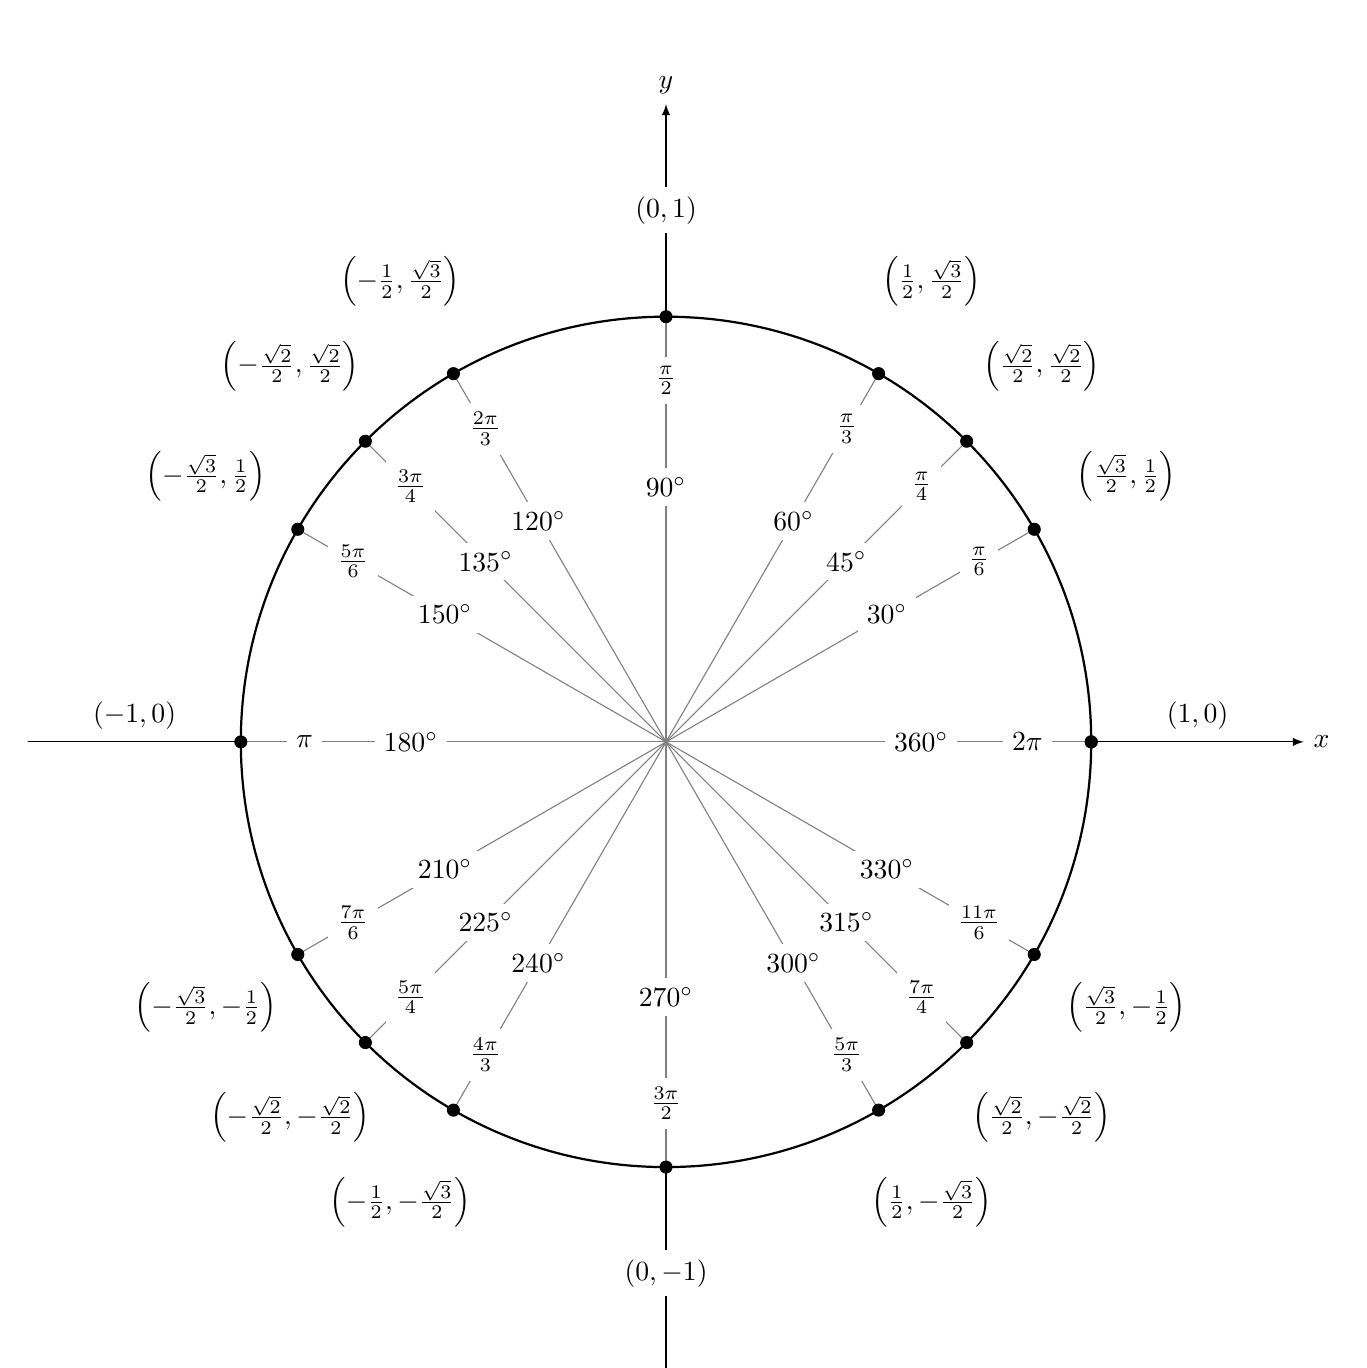
\begin{tikzpicture}[scale=5.4,cap=round,>=latex]
    % draw the coordinates
    \draw[->] (-1.5cm,0cm) -- (1.5cm,0cm) node[right,fill=white] {$x$};
    \draw[->] (0cm,-1.5cm) -- (0cm,1.5cm) node[above,fill=white] {$y$};

    % draw the unit circle
    \draw[thick] (0cm,0cm) circle(1cm);

    \foreach \x in {0,30,45,60,90,120,135,150,180,210,225,240,270,300,315,330,360} {%this is the manual way, includes the 45degree lines
    % \foreach \x in {0,30,...,360} {%this is the default, leave out the 45degree lines
      % lines from center to point
      \draw[gray] (0cm,0cm) -- (\x:1cm);
      % dots at each point
      \filldraw[black] (\x:1cm) circle(0.4pt);
      % draw each angle in degrees
      \draw (\x:0.6cm) node[fill=white] {$\x^\circ$};
    }

    % draw each angle in radians
    \foreach \x/\xtext in {
      30/\frac{\pi}{6},
      45/\frac{\pi}{4},
      60/\frac{\pi}{3},
      90/\frac{\pi}{2},
      120/\frac{2\pi}{3},
      135/\frac{3\pi}{4},
      150/\frac{5\pi}{6},
      180/\pi,
      210/\frac{7\pi}{6},
      225/\frac{5\pi}{4},
      240/\frac{4\pi}{3},
      270/\frac{3\pi}{2},
      300/\frac{5\pi}{3},
      315/\frac{7\pi}{4},
      330/\frac{11\pi}{6},
      360/2\pi}
    \draw (\x:0.85cm) node[fill=white] {$\xtext$};

    \foreach \x/\xtext/\y in {
      % the coordinates for the first quadrant
      30/\frac{\sqrt{3}}{2}/\frac{1}{2},
      45/\frac{\sqrt{2}}{2}/\frac{\sqrt{2}}{2},
      60/\frac{1}{2}/\frac{\sqrt{3}}{2},
      % the coordinates for the second quadrant
      150/-\frac{\sqrt{3}}{2}/\frac{1}{2},
      135/-\frac{\sqrt{2}}{2}/\frac{\sqrt{2}}{2},
      120/-\frac{1}{2}/\frac{\sqrt{3}}{2},
      % the coordinates for the third quadrant
      210/-\frac{\sqrt{3}}{2}/-\frac{1}{2},
      225/-\frac{\sqrt{2}}{2}/-\frac{\sqrt{2}}{2},
      240/-\frac{1}{2}/-\frac{\sqrt{3}}{2},
      % the coordinates for the fourth quadrant
      330/\frac{\sqrt{3}}{2}/-\frac{1}{2},
      315/\frac{\sqrt{2}}{2}/-\frac{\sqrt{2}}{2},
      300/\frac{1}{2}/-\frac{\sqrt{3}}{2}}
    \draw (\x:1.25cm) node[fill=white] {$\left(\xtext,\y\right)$};

    % draw the horizontal and vertical coordinates
    % the placement is better this way
    \draw (-1.25cm,0cm) node[above=1pt] {$(-1,0)$}
    (1.25cm,0cm)  node[above=1pt] {$(1,0)$}
    (0cm,-1.25cm) node[fill=white] {$(0,-1)$}
    (0cm,1.25cm)  node[fill=white] {$(0,1)$};
  \end{tikzpicture}
\end{figure}
%%% Local Variables:
%%% mode: latex
%%% TeX-master: "../main"
%%% End:
%unit circle
%NOTE: cannot nest \include{} statements, that's why \clearpage\input{} is used instead
%%% Local Variables:
%%% mode: latex
%%% TeX-master: "../main"
%%% End:
%app.02: quick reference information
%%note header stored in prob-solving
\begin{longtable}{p{0.5\textwidth} p{0.5\textwidth}}
    \tablesection{Appendix III: List of Problem-Solving Strategies}
	\tablesubsection{General Physics Problem-Solving Strategy} 
    & \\%needed for formatting
\end{longtable}
\vspace{-1cm}
\par Excerpt from \url{http://www.people.fas.harvard.edu/~djmorin/chap1.pdf}

\begin{enumerate}
	\item \textbf{Draw a Diagram} In the diagram, be sure to clearly label all the relevant quantities (forces, lengths, masses, etc). Diagrams are absolutely critical in certain types of problems. For example, in problems involving free-body diagrams or relativistic kinematics, drawing a diagram can change a hopelessly complicated problem into a near-trivial one. And even in cases where diagrams aren't this crucial, they're invariable very helpful. A picture is definitely worth a thousand words (and even a few more, if you label things!).
    \item \textbf{Record Known \& Unknown Quantities} In a simple problem, you may just do this in your head without realizing it. But in more difficult problems, it is very useful to explicitly write things out. For example, if there are three unknowns that you are trying to find, but you've written down only two facts, then you know there must be another you're missing, so you can go searching for it. It might be a conservation law, or an \(F=ma\) equation, etc.
    \item \textbf{Solve Things Symbolically} If you are solving a problem where the given quantities are specified numerically, you should immediately change the numbers to letters and solve the problem in terms of the letters. After you obtain an answer in terms of the letters, you can plug in the actual numerical values to obtain a numerical answer. That said, it should be noted that there are occasionally times when things get a bit messy when working with letters. For example, solving a system of three equations in three unknowns might be rather cumbersome unless you plug in the actual numbers. But in the vast majority of problems, it is highly advantageous to work entirely with letters.
    \item \textbf{Consider Units \& Dimensions} The units, or dimensions, of a quantity are the powers of mass, length, and time associated with it. For example, the units of speed are length per time. The consideration of units offers two main benefits. First, looking at units before you start a problem can tell you roughtly what the answer has to look like, up to numerical factors. Second, checking units at the end of a calculation (which is something you should \textit{always} do) can tell you if your answer has a chance at being correct. It won't tell you that your answer is definitely correct, but it might tell you that your answer is definitely incorrect. For example, if your goal in a problem is to find a length, and you end up with a mass, then you know it's time to look back over your work.
    \item \textbf{Check Limiting \& Special Cases} As with units, the consideration of limiting cases (or special cases) offers two main benefits. First, it can help you get started on a problem. If you're having trouble figuring out how a given system behaves, then you can imagine making, for example, a certain length become very large or very small, and then you can see what happens to the behaviour. Having convinced yourself that the length actually affects the system in extreme cases (or perhaps you will discover that the length doesn't affect things at all, it will then be easier to understand how it affects the system in general, which will then make it easier to write down the relevant quantitative equations (conservation laws, \(F=ma\) equations, etc.), which will allow you to fully solve the problem. In short, modifying the various parameters and seeing the effects on the system can lead to an enormous amount of information. Second, as with checking units, checking limiting cases (or special cases) is something you should \textit{always} do at the end of a calculation. But as with checking units, it won't tell you that your answer is definitely correct, but it might tell you that your answer is definitely incorrect. It is generally true that your intuition about limiting cases is much better than your intuition about generic values of the parameters. you should use this fact to your advantage.
    \item \textbf{Use Your Brain} Whenever you end up with a numerical answer to a problem, be sure to do a sanity check to see if the number is reasonable. If you've calculated the distance along the ground that a car skids before it comes to rest, and if you've gotten answer of a kilometer or a millimeter, then you know you've probably done something wrong. Errors of this sort often come from forgetting some powers of $10$ (say when converting kilometers to meters) or from multiplying something instead of dividing (although you should be able to catch this by checking your units too).
\end{enumerate}
\newpage%app.03: problem solving strategies
%--removed the problem solving strats because the purpose of the sheet isn't to teach physics but to be a resource for physics

\end{document}